\documentclass[a4paper,12pt]{book}
\usepackage{graphicx} % For graphics
\usepackage{float}
\usepackage{comment}
\usepackage{tikz}
\usepackage{tkz-euclide} % Add this line to include the tkz-euclide package
\usetikzlibrary{calc}
\usetikzlibrary{matrix}
\usetikzlibrary{angles,quotes} % For drawing and labeling angles
\usepackage{siunitx}
\usepackage{amsmath}
\usepackage{enumitem}
\usepackage{amssymb}
\usepackage{pgfplots}
\pgfplotsset{compat=newest}

% Define custom styles for holdot and soldot
\tikzset{
    holdot/.style={color=black,only marks,mark=*},
    soldot/.style={color=black,fill=white,only marks,mark=*},
}

\usepgfplotslibrary{fillbetween} 

% Configure hyperref package to color links blue
\usepackage[colorlinks=true, linkcolor=blue, citecolor=blue, urlcolor=blue]{hyperref}

\newcommand{\inputtoc}[1]{\input{#1}}

% \makeindex % Command to make the index

\pgfmathdeclarefunction{csc}{1}{%
  \pgfmathparse{1/sin(#1)}%
}

\newenvironment{exercise}[1][]
  {\par\medskip\noindent\textbf{Exercise #1} \rmfamily}
  {\medskip}

% Define the problem environment
\newcounter{problem}
\newenvironment{problem}[1][\theproblem]
{\refstepcounter{problem}\par\medskip\noindent\textbf{Problem~#1:} \rmfamily}{\medskip}

% Define the solution environment
\newenvironment{solution}[1][]
{\par\noindent\textit{Solution:} \rmfamily}{\medskip}

% Define the example environment
\newcounter{example}
\newenvironment{example}[1][\theexample]
  {\refstepcounter{example}\par\medskip\noindent\textbf{Example~#1:} \rmfamily}
  {\medskip}
  
% Define theorem, application, definition, method, and discussion environments
\newtheorem{theorem}{Theorem}
\newtheorem{application}{Application}
\newtheorem{definition}{Definition}
\newtheorem{method}{Method}
\newtheorem{discussion}{Discussion}

\begin{document}

% --- Book Cover ---
\begin{titlepage}
    \begin{tikzpicture}[remember picture, overlay]
        % Background color
        \fill[cyan!30] (current page.south west) rectangle (current page.north east);

        % Decorative Circles Pattern at the bottom
        \foreach \i in {0,...,36}
        {
            \fill[cyan!40, rotate around={10*\i:(current page.center)}] 
                (current page.south) circle (1cm);
        }
        
        % Title and additional info
        \node at (current page.center) [font=\Huge, text width=0.8\textwidth, align=center] 
            {\textbf{Pre-Calculus in Brief with Python, Colab, GitHub, and \LaTeX  \\ PCiB - Version 0.65}};
            
        \node[align=center, font=\large] at (current page.center) 
            [yshift=-2.5cm] {\today}; % <- This is the compilation date
            
        \node[align=center, font=\large] at (current page.center) 
            [yshift=-3.5cm] {MIT License};
        
        \node[align=center, font=\large] at (current page.center) 
            [yshift=-5cm] {Available on GitHub at: \\ 
            \url{https://GitHub.com/nicholaskarlson/PCiB}};
    \end{tikzpicture}
\end{titlepage}

% --- Table of Contents ---
\tableofcontents
\cleardoublepage

% --- Preface ---
\chapter*{Preface}
\addcontentsline{toc}{chapter}{Preface}
This text, \emph{Pre-Calculus in Brief - PCiB} aspires to be more than just another math book. This book strives to foster collaborative math writing. Note that this book has very few references. The reader is encouraged to use resources available on the Web to fact-check. This book's view on ``causation'' and facts is heavily influenced by Mosteller and Tukey \cite{mosteller1977}.

\section*{Redefining the Role of the Reader}
Pre-Calculus in Brief (PCiB) is an endeavor to reshape how math is written, understood, and studied. It's not just a passive read but an open-source approach to math, aiming to encourage students to become proactive learners.

This project strives to break the traditional mold of math education and invites readers and professional mathematicians to participate actively.

\section*{A Dynamic Relationship with Math}
\emph{Pre-Calculus in Brief} is not just a book but a movement and methodology, heralding a new era in how we approach, consume, and interact with math. By positioning the reader as an integral part of the math-book process, PCiB fosters a dynamic relationship with math, making mathematics more accessible, proactive, and relevant. In this shifting paradigm, we are all potential mathematicians, creators of interesting and relevant ways to learn and study math.

Please fork the LaTeX source code for PCiB (available on GitHub) and create your own book that chooses the facts and exercises most relevant to you! Also, starring the PCiB project on GitHub would be greatly appreciated! Thanks for reading PCiB!

% --- Chapters ---
\chapter{Introduction to PCiB}
\subsection*{Welcome to PCiB on GitHub}
Pre-Calculus in Brief, abbreviated PCiB, isn't merely a passive read. It's an endeavor to reshape how math is written, studied, and taught. By presenting an open-source approach to math, the goal is to encourage everyone to become proactive readers and writers of math. 

\subsection*{Fostering a Proactive Engagement with Math}

\emph{Pre-Calculus in Brief} is a call for a renewed engagement with mathematics. PCiB is an endeavor to reshape how math is written, understood, and studied. It's not just a passive read but an open-source approach to math, aiming to encourage students to become proactive learners.

This project strives to break the traditional mold of math education and encourages readers and professional mathematicians to participate actively.

\bigskip
\noindent
Please fork the \LaTeX{} source code for PCiB (available on GitHub) and create your own book on Pre-Calculus that chooses the content most relevant to you! Also, starring the PCiB project on GitHub would be greatly appreciated! Thanks for reading PCiB!

\chapter{Open-Source Ethos}
\section*{The Spirit of Shared Knowledge and Collaboration}
Math, like software, is better when it's open. PCiB draws inspiration from the open-source software movement; this section elucidates how a collaborative, transparent, and shared approach can enhance our understanding of math. Here, we look at the philosophy behind open-source and how it beautifully combines with the study of mathematics.

\subsection*{Open-Source Math: Preserving Tradition Through Collaborative Exploration}
Mathematics, like software, thrives when it embraces openness and transparency. PCiB takes a leaf from the proven benefits of the open-source software model; this section highlights how a collaborative and transparent method can improve and deepen our grasp of math and its texts. Here, we explore the principles of open source and how these principles align with the development of mathematics and its texts.

\subsection*{Understanding the Open-Source Ethos}
The open-source paradigm revolves around shared ownership, collaboration, and the free exchange of knowledge. In the software realm, this approach has led to groundbreaking innovations built and enhanced by a global community of skilled contributors. United by a mutual objective, these individuals pool their diverse talents and insights to improve and share software solutions for broader public benefit.

\subsection*{Advantages of the Open-Source Framework in Math}
\subsubsection*{Collective Insight}
Mirroring the collaborative essence of open-source software, many individuals can offer their perspectives and knowledge, making math texts more robust and varied.

\subsubsection*{Enhancement and Accuracy}
Open platforms foster an environment of constructive criticism, ensuring prompt identification and correction of inaccuracies. This meticulous peer review can help provide a credible and current mathematical text.

\subsubsection*{Universal Access}
Much as open-source software promotes free access and modification, open-source math prioritizes universal accessibility. This ensures mathematics knowledge isn't restricted to a select few but is available to all curious minds.

\subsection*{Potential Challenges}
Despite its advantages, melding open-source with math has potential pitfalls. The volume of contributions can complicate accuracy verification processes. 

However, the very community championing this open-source approach to math can serve as its vigilant protector. They can ensure that contributions undergo rigorous evaluation and referencing, akin to the meticulous checks within the open-source software community.

\subsection*{Conclusion: Reinvigorating Our Experience with Math}
Adopting an open-source perspective to the approach of math signifies a refreshed approach. It beckons a worldwide community to collaborate and forge a comprehensive and exciting math text. In this refreshed approach, every individual can play a part, both as a contributor and a learner. Math texts, through this lens, evolve and flourish, reflecting the collective input of active participants.

\chapter{Introduction to GitHub}
\section*{The Hub for Modern Collaboration}
\subsection*{Harnessing GitHub: A New Frontier in Collaborative Math Writing}
At the heart of our collaborative math endeavor lies GitHub, a platform traditionally associated with code but now repurposed for our endeavor. This section provides a primer on GitHub, laying the foundation for those unfamiliar and offering insights into its transformative potential for collective math writing, learning, and teaching.

\subsection*{A Brief Introduction to GitHub}
Originally conceptualized as a platform for developers, GitHub is a repository hosting service that facilitates version control using Git. At its core, it allows multiple users to work on a project simultaneously, tracking changes and ensuring that the latest version of a project is always accessible. Over the years, GitHub has grown beyond its initial software-centric confines, becoming a hub for all kinds of collaborative projects, from writing to data science and now to math.

\subsection*{Repurposing GitHub for Math Texts}
\subsubsection*{Version Control}
Math writing, like software, is dynamic and constantly evolving. As new sources or perspectives emerge, math texts may need revisions. GitHub's version control ensures that every change made to a document is tracked, enabling mathematicians to see how math texts evolve over time.

\subsubsection*{Collaborative Writing}
Multiple contributors can work on a single math text simultaneously. This multi-user capability ensures diverse viewpoints can be seamlessly integrated, making the math text richer and more comprehensive.

\subsubsection*{Review and Feedback}
Just as developers review and comment on code, mathematicians can provide feedback on written content. This feature encourages rigorous peer review, ensuring accuracy and credibility.

\subsubsection*{Open Access}
Math texts on GitHub can be made public, granting anyone access to read, contribute, or fork the text into their own versions. This workflow democratizes math texts, making the creation process a collective endeavor rather than the domain of a select few.

\subsubsection*{Transparency}
All changes and contributions are logged, providing a clear trail of the evolution of a mathematical text. This transparency bolsters the credibility of the text hosted on the platform.

\subsubsection*{Community Building}
Beyond just writing, GitHub fosters a community of mathematicians, enthusiasts, and readers who can discuss, debate, and engage in meaningful dialogues about math and available math texts on GitHub.

\subsection*{Conclusion: Envisioning a Collaborative Mathematical Landscape}
Embracing GitHub as a tool for collaborative math signifies more than just a shift in approach; it heralds a new era of inclusivity, transparency, and dynamism in writing, learning, and math teaching. 

\chapter{Encouragement to Fork}
\subsection*{Invitation to Dive Deep and Make It Your Own}
PCiB isn't a static entity. It thrives on evolution, adaptation, and diversification, much like math itself. We encourage readers to "fork" (a term soon to be discussed) and create their own versions of this book. Read this section to understand the essence of "forking" and how it can be the starting point of your unique math journey.

\subsection*{The Concept of Forking: A Brief Overview}

In the realm of software development, particularly in platforms like GitHub, "forking" refers to the act of creating a copy of a project, allowing one to make changes independently of the original. In this context, forking PCiB enables readers to take the base content and adapt, modify, and expand upon it, tailoring the narrative to resonate with their perspectives, insights, and understanding.

\subsection*{How to Begin Your Forking Journey}

Start Small: You don't need to rewrite entire chapters. Begin by adding annotations, insights, or even footnotes to existing content. As you grow more confident, you can expand and modify larger sections.

Engage with the Community: Share your forked version with other readers. This encourages discourse, debate, and constructive feedback, allowing your text to be refined and enhanced.

Celebrate input: Encourage others around you to fork and create their own versions. The more in-depth the input, the deeper our collective understanding of math potentially becomes.

\subsection*{Conclusion: The Power of Collective Math}

The invitation to fork PCiB isn't just about creating different versions of a book. It's a call to embrace collective writing, learning, and teaching. By embracing the essence of forking, math is not just something we read but something we actively shape, share, and pass on.

\chapter{More About GitHub}
\section*{Discovering the Power of Collaborative Tools}
Diving deeper into the world of GitHub, this chapter provides a comprehensive overview. Beyond its technicalities, we explore how GitHub emerged as a revolutionary platform for collaboration and how it can be leveraged for those interested in writing, teaching, and learning about math.

\subsection*{The Genesis of GitHub}
GitHub began as a platform designed for software developers to manage and track changes to their codebase. Launched in 2008, it swiftly gained traction due to its user-friendly interface and efficient version control system powered by Git. Over the years, it evolved from a mere repository hosting service to a dynamic hub of collaboration, housing millions of projects and engaging tens of millions of users worldwide.

\subsection*{GitHub: More than Just Code}
While GitHub's origins are rooted in code collaboration, its adaptable nature has made it a favored platform for various non-code projects. Writers, designers, educators, and researchers have discovered the potential of GitHub as a tool for:

\subsubsection*{Document Collaboration}
With its built-in version control, contributors can track changes, revert to previous versions, and seamlessly merge updates.

\subsubsection*{Project Management}
With features like "issues" and "milestones," teams can organize tasks, set goals, and monitor progress.

\subsubsection*{Open Access \& Transparency}
Public repositories allow for open contributions, ensuring transparency and fostering a sense of collective ownership.

\subsubsection*{Collaborative Writing}
Multiple contributors can simultaneously work on a single document, with every change being tracked and attributed, facilitating teamwork on extensive projects like books or research papers.

\subsubsection*{Engaging the Public}
With the platform's inherent transparency, researchers can make their work-in-progress accessible to the public, inviting insights, corrections, and contributions.

\subsection*{Case Study: PCiB's Use of GitHub}
PCiB's journey on GitHub is a testament to the platform's potential in mathematical endeavors. By hosting the book on GitHub, the following is possible:

\subsubsection*{Feedback Loop}
Readers can raise "issues," pointing out inaccuracies, suggesting enhancements, or even recommending new sections or topics.

\subsubsection*{Forking}
As previously discussed, readers can "fork" the repository, creating their unique versions of the book while staying connected to the original.

\subsubsection*{Regular Updates}
With math being dynamic, the book can be regularly updated, with new versions being released as and when significant changes are incorporated.

\subsection*{Challenges and Considerations}
While GitHub offers many advantages, it's essential to understand its limitations:

\subsubsection*{Learning Curve}
For those unfamiliar with Git or version control, there can be an initial learning curve.

\subsubsection*{Data Overwhelm}
With vast amounts of data and contributions, ensuring quality and accuracy can be challenging.

\subsubsection*{Diverse Audience Management}
Catering to both tech-savvy and non-tech audiences might require creating additional resources or tutorials to ensure inclusivity.

\subsection*{Conclusion: GitHub – A Paradigm Shift in Collaboration}
The rise of GitHub marks a significant shift in how we perceive and participate in collaborative projects. Its adaptability, transparency, and user-centric design make it a powerful tool, not just for coders but for anyone passionate about collective endeavors. In the realm of mathematics, GitHub promises a future where texts are continually refined, expanded, and enriched by a global community.

\chapter{Forking Process}
\section*{The Heart of Collaboration on GitHub}
The beauty of open-source lies in its democratization of content creation. In this section, we demystify the process of "forking" on GitHub, guiding you step-by-step on how to take PCiB and create a version uniquely yours.

\subsection*{Understanding Forking}
Before diving into the specifics, it's crucial to understand what "forking" means in the context of GitHub. In the simplest terms, to "fork" a project means to create a personal copy of someone else's project. Forking allows you to freely experiment with changes without affecting the original project. Forking is akin to taking a book you admire and making a copy to write your notes, edits, or additional chapters without altering the original book.

\subsection*{Why Fork?}
\subsubsection*{Experimentation}
It provides a safe space where you can test out ideas, make changes, or introduce new content.

\subsubsection*{Personalization}
For projects like PCiB, it allows readers to customize the content, tailor it to their perspectives, or even localize it for specific audiences.

\subsubsection*{Collaboration}
If you believe your changes have broad appeal, you can propose that they be incorporated back into the original project, enriching it with your unique contributions.

\subsection*{Step-by-Step Forking Guide}
\subsubsection*{Set Up Your GitHub Account}
If you don't have an account on GitHub, you'll need to create one. Visit GitHub's official site and sign up.

\subsubsection*{Navigate to the PCiB Repository}
Once logged in, search for the PCiB project or navigate to its URL directly.

\subsubsection*{Click the 'Fork' Button}
The fork button is located at the top right corner of the repository page; this button will create a copy of PCiB in your account.

\subsubsection*{Clone Your Forked Repository}
Forking allows you to have a local copy on your computer, making editing and experimentation easier. Use the command: \texttt{git clone [URL of your forked repo]}.

\subsubsection*{Make Your Changes}
Using your preferred tools, introduce the edits, additions, or modifications you desire.

\subsubsection*{Commit and Push Changes}
Once satisfied, save these changes (known as a "commit") and then "push" them to your forked repository on GitHub.

\subsubsection*{Optional – Create a Pull Request}
If you believe your changes should be incorporated into the original PCiB repository, you can create a "pull request." A pull request notifies the original authors of your suggestions.

\subsection*{Things to Keep in Mind}
\subsubsection*{Stay Updated}
The original PCiB project may undergo updates. It's a good practice to regularly "pull" from the original repo to keep your fork up-to-date.

\subsubsection*{Engage with the Community}
Open-source thrives on community interactions. Engage in discussions, seek feedback, and please remain open to constructive criticism.

\subsection*{Conclusion: Embracing the Forking Culture}
Forking is more than just a technical process; it symbolizes the ethos of open-source — a world where knowledge is not hoarded but shared, refined, and built upon collectively. By forking PCiB or any other project, you're not just creating a personal copy; you're becoming a part of a global movement that values collaboration, innovation, and the shared pursuit of knowledge. So, embark on this journey, make your unique mark, and contribute to the ever-evolving corpus of collective wisdom.

\chapter{Editing and Customizing}
\section*{Tailoring Repositories to Suit Your Needs}
Now, let's build upon the forking process; this segment delves into the next steps. How can you edit and customize your version of PCiB? What tools and techniques are available at your disposal? Embark on this informative journey as we guide you through the intricacies of editing on GitHub.

\subsection*{Understanding the GitHub Workspace}
Before diving into the specifics of editing, it's essential to familiarize yourself with the GitHub workspace. Think of it as a digital toolshed where each tool serves a unique function:

\begin{itemize}
    \item \textbf{Repository (Repo)}: This is the project's main folder where all your project's files are stored and where you track all changes.
    \item \textbf{Branches}: These are parallel versions of a repository, allowing you to work on features or edits without altering the main project.
    \item \textbf{Commits}: This is a saved change in the repository, akin to saving a file after making edits.
    \item \textbf{Pull Requests}: This is how you notify the main project of desired changes, proposing that your edits be merged with the original.
\end{itemize}

\subsection*{Editing Files Directly on GitHub}
For minor changes, you might opt to edit directly on GitHub:

\begin{enumerate}
    \item Navigate to the File: Within your forked PCiB repository, find the file you want to edit.
    \item Click the Pencil Icon: This button allows you to edit the file.
    \item Make Your Edits: Modify the content as needed.
    \item Save and Commit: Below the editing pane, you'll see a "commit changes" section. Add a brief note summarizing your changes and click 'Commit.'
\end{enumerate}

\subsection*{Editing Files Locally}
For extensive customization:

\begin{enumerate}
    \item Clone Your Repository: Use a tool like Git to clone (download) your forked repo to your local computer.
    \item Edit Using Your Preferred Tools: This could range from text editors to specialized software, depending on the file type.
    \item Commit and Push: After making your changes, save them (commit) and then upload (push) them to your GitHub repository.
\end{enumerate}

\subsection*{Utilizing Branches for Extensive Customization}
Branches are especially useful for significant overhauls or when working on different versions:

\begin{enumerate}
    \item Create a New Branch: From your main project page, use the branch dropdown to type in a new branch name and create it.
    \item Switch to Your Branch: Ensure you're working in this new parallel environment.
    \item Make and Commit Changes: As you would in the main project.
    \item Merging: Once satisfied with your edits in the branch, you can merge these changes back into the main project or keep them separate as a different version.
\end{enumerate}

\subsection*{Exploring Additional Tools and Extensions}
GitHub's ecosystem is rich with tools and extensions to enhance your editing experience:

\begin{itemize}
    \item \textbf{GitHub Desktop}: An application that simplifies the process of managing your repositories without using command-line tools.
    \item \textbf{Markdown Editors}: Since many GitHub files (like READMEs) are written in Markdown, tools like StackEdit or Dillinger can be invaluable.
    \item \textbf{Extensions for Browsers}: Tools like Octotree can help in navigating repositories more effortlessly.
\end{itemize}

\subsection*{Conclusion: The Art of Tailored Content}
Editing and customizing on GitHub might seem daunting initially, but with practice, it transforms into a manageable workflow. Many people find that the ability to take a project like PCiB and mold it into something uniquely theirs is empowering. It's a testament to the open-source community's ethos, where shared knowledge becomes the canvas and our collective edits, the brushstrokes, crafting an ever-evolving masterpiece. As you embark on your customization journey, remember that every edit, no matter how small, contributes to the project potentially in significant ways.

\chapter{Engaging with the Community}
\section*{Joining the Global Conversation}

\subsection*{The Significance of the GitHub Community}
The digital age has bestowed upon us the gift of connectivity. On platforms like GitHub, this connectivity transcends borders, disciplines, and ideologies, culminating in a melting pot of diverse ideas and knowledge. For mathematicians and math enthusiasts, GitHub offers a space not only to store and manage content but also to engage with an audience that is passionate, informed, and eager to contribute.

\subsection*{1. Discussions and Debates}
One of the most enriching aspects of the GitHub community is the plethora of discussions that unfold:

\begin{itemize}
    \item \textbf{Issues}: A core feature of GitHub, "issues" allow users to raise questions, report problems, or propose enhancements. 
    \item \textbf{GitHub Discussions}: A newer feature, Discussions, acts like a community forum. It's an excellent place for extended conversations, brainstorming, and sharing ideas or resources.
\end{itemize}

\subsection*{2. Collaborative Content Creation}
Beyond solitary endeavors, GitHub shines in its collaborative capabilities:

\begin{itemize}
    \item \textbf{Pull Requests}: If you have made an alteration to a math text or added a new perspective, pull requests are the way to propose these changes to the original repository owner. Pull requests foster a collaborative spirit, where content isn't static but continually evolving with community input.
    \item \textbf{Fork and Merge}: As you've learned, forking allows you to create your version of a repository. Engaging with the Community means you can merge changes from others into your fork, blending a mixture of diverse insights.
\end{itemize}

\subsection*{3. Building and Nurturing Networks}
Connections made on GitHub often spill over into lasting professional relationships:

\begin{itemize}
    \item \textbf{Following and Followers}: Like on social media platforms, you can follow contributors whose work resonates with you. Following contributors creates a curated feed of updates and also allows you to be part of a more extensive network.
    \item \textbf{GitHub Stars}: If a particular project or repository impresses you, give it a star! Starring not only bookmarks the project for you but also shows appreciation to the creator.
\end{itemize}

\subsection*{4. Learning and Growing Through Feedback}
The Community's feedback is an invaluable asset:

\begin{itemize}
    \item \textbf{Code Reviews}: Although traditionally for software, text writers can use this feature to receive feedback on their methodologies or approaches, refining their work.
    \item \textbf{Community Insights}: The "insights" tab on a repository provides analytics. For text writers, this can give a sense of which topics garner more attention and interest.
\end{itemize}

\subsection*{5. Participating in Community Events}
GitHub often hosts and sponsors events:

\begin{itemize}
    \item \textbf{Hackathons}: While traditionally for coders, these events can be repurposed for text writer content creation, where participants collaboratively tackle projects or themes.
    \item \textbf{Webinars and Workshops}: These events can range from mastering GitHub's technical side to thematic discussions on math topics.
\end{itemize}

\subsection*{A Project of Collective Wisdom}
Math, in many ways, is a collective endeavor. GitHub can provide a dynamic Community. By engaging with this Community you can become an active participant in the creation of mathematical texts.

\chapter{Pre-Calculus Basic Topics}
\subsection*{Introduction}
In this chapter, we start talking about actual pre-calculus topics. Here we will introduce geometry, algebra, and trigonometry, with details provided in later chapters.

\chapter{Essential Geometry for Calculus}
\label{chap:geometry_for_calculus}


Geometry, with its focus on shapes, sizes, and the properties of space, is fundamental to understanding and applying calculus concepts. In this chapter, we explore key geometric principles and their applications in calculus.


\section{Coordinate Geometry}
\label{sec:coordinate_geometry}
Coordinate geometry, or analytic geometry, combines algebra and geometry. It is crucial for calculus. In this section, we will delve into the fundamental aspects of coordinate geometry, illustrating each concept with diagrams and graphs.

\subsection{The Cartesian Plane}
\label{subsec:the_cartesian_plane}
The Cartesian plane is a two-dimensional plane formed by the intersection of a vertical line (y-axis) and a horizontal line (x-axis). Points on this plane are identified by coordinates (x, y).

\begin{figure}[H]
\centering
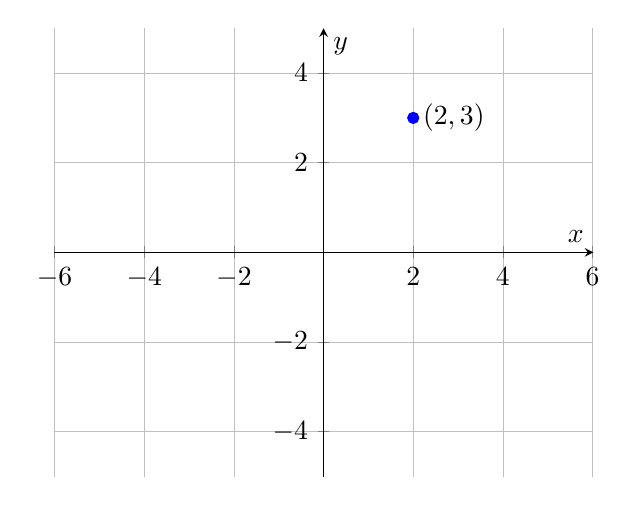
\begin{tikzpicture}
\begin{axis}[
    axis lines=middle,
    xlabel={$x$},
    ylabel={$y$},
    xmin=-5, xmax=5,
    ymin=-5, ymax=5,
    grid=both,
    grid style={line width=.1pt, draw=gray!10},
    major grid style={line width=.2pt,draw=gray!50},
    axis equal
]
\addplot[mark=*,color=blue] coordinates {(2,3)};
\node at (axis cs:2,3) [anchor=west] {$(2,3)$};
\end{axis}
\end{tikzpicture}
\caption{A point $(2,3)$ on the Cartesian plane}
\end{figure}

\subsection{Graphing Linear Equations}
\label{subsec:graphing_linear_equations}
Linear equations in two variables can be graphed on the Cartesian plane. The graph of a linear equation forms a straight line.

% Example of graphing a linear equation
\begin{figure}[H]
\centering
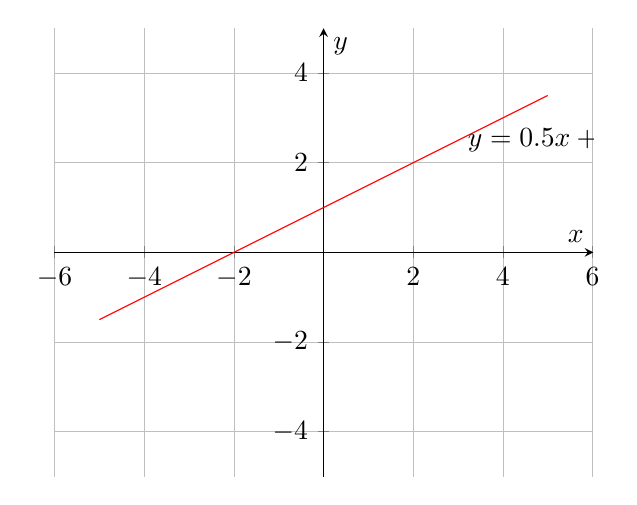
\begin{tikzpicture}
\begin{axis}[
    axis lines=middle,
    xlabel={$x$},
    ylabel={$y$},
    xmin=-5, xmax=5,
    ymin=-5, ymax=5,
    grid=both,
    grid style={line width=.1pt, draw=gray!10},
    major grid style={line width=.2pt,draw=gray!50},
    axis equal
]
\addplot[domain=-5:5, samples=100, color=red]{0.5*x + 1};
\node at (axis cs:3,2.5) [anchor=west] {$y = 0.5x + 1$};
\end{axis}
\end{tikzpicture}
\caption{Graph of the linear equation $y = 0.5x + 1$}
\end{figure}

\subsection{Slope of a Line}
\label{subsec:slope_of_a_line}
The slope of a line is a measure of its steepness and direction. It is defined as the ratio of the change in y to the change in x between two points on the line.

% Slope illustration
\begin{figure}[H]
\centering
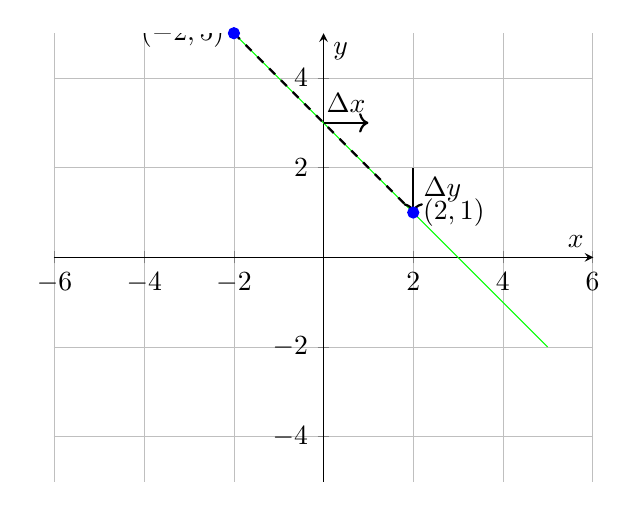
\begin{tikzpicture}
\begin{axis}[
    axis lines=middle,
    xlabel={$x$},
    ylabel={$y$},
    xmin=-5, xmax=5,
    ymin=-5, ymax=5,
    grid=both,
    grid style={line width=.1pt, draw=gray!10},
    major grid style={line width=.2pt,draw=gray!50},
    axis equal
]
\addplot[domain=-5:5, samples=100, color=green]{-x + 3};
\addplot[mark=*,color=blue] coordinates {(-2,5)};
\addplot[mark=*,color=blue] coordinates {(2,1)};
\draw[thick, dashed] (axis cs:-2,5) -- (axis cs:2,1);
\node at (axis cs:-2,5) [anchor=east] {$(-2,5)$};
\node at (axis cs:2,1) [anchor=west] {$(2,1)$};
\draw[->,thick] (axis cs:0,3) -- (axis cs:1,3) node[midway, above] {$\Delta x$};
\draw[->,thick] (axis cs:2,2) -- (axis cs:2,1) node[midway, right] {$\Delta y$};
\end{axis}
\end{tikzpicture}
\caption{Illustration of the slope of a line}
\end{figure}

\begin{exercise}
Calculate the slope of the line connecting points $(-2, 5)$ and $(2, 1)$.
\end{exercise}

% Add more subsections and exercises as required

% --- End of Coordinate Geometry Section ---

% Example Problems for Coordinate Geometry Section

\section*{Example Problems}
\label{sec:example_problems_coordinate_geometry}
To further solidify your understanding of coordinate geometry, here are some example problems with solutions.

\begin{problem}[1]
Find the coordinates of the midpoint of the line segment joining the points \(A(1, 2)\) and \(B(4, 6)\).
\end{problem}

\begin{solution}
The midpoint \(M\) of a line segment with endpoints \(A(x_1, y_1)\) and \(B(x_2, y_2)\) is given by the formula:
\[ M = \left( \frac{x_1 + x_2}{2}, \frac{y_1 + y_2}{2} \right) \]
Substituting the given values:
\[ M = \left( \frac{1 + 4}{2}, \frac{2 + 6}{2} \right) = \left( \frac{5}{2}, 4 \right) \]
Therefore, the coordinates of the midpoint are \(\left( \frac{5}{2}, 4 \right)\).
\end{solution}

\begin{problem}[2]
Determine the slope of the line passing through the points \((3, -2)\) and \((7, 6)\).
\end{problem}

\begin{solution}
The slope \(m\) of the line passing through points \((x_1, y_1)\) and \((x_2, y_2)\) is calculated as:
\[ m = \frac{y_2 - y_1}{x_2 - x_1} \]
Substituting the given points:
\[ m = \frac{6 - (-2)}{7 - 3} = \frac{8}{4} = 2 \]
Hence, the slope of the line is \(2\).
\end{solution}

\begin{problem}[3]
Graph the linear equation \(2x - 3y = 6\) on the Cartesian plane.
\end{problem}

\begin{solution}
To graph the equation \(2x - 3y = 6\), first solve for \(y\):
\[ 3y = 2x - 6 \]
\[ y = \frac{2}{3}x - 2 \]
Now plot two or more points that satisfy the equation and draw the line through them.

\begin{figure}[H]
\centering
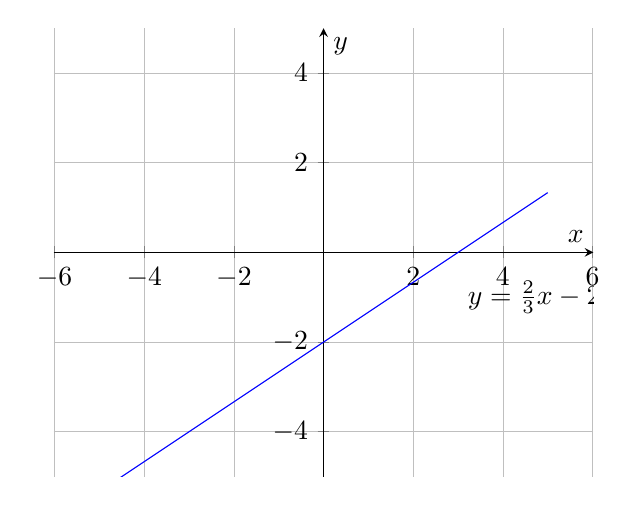
\begin{tikzpicture}
\begin{axis}[
    axis lines=middle,
    xlabel={$x$},
    ylabel={$y$},
    xmin=-5, xmax=5,
    ymin=-5, ymax=5,
    grid=both,
    grid style={line width=.1pt, draw=gray!10},
    major grid style={line width=.2pt,draw=gray!50},
    axis equal
]
\addplot[domain=-5:5, samples=100, color=blue]{(2/3)*x - 2};
\node at (axis cs:3,-1) [anchor=west] {$y = \frac{2}{3}x - 2$};
\end{axis}
\end{tikzpicture}
\caption{Graph of the equation \(2x - 3y = 6\)}
\end{figure}
\end{solution}

% --- End of Examples


\subsection{The Cartesian Plane - Details}
\label{subsec:the_cartesian_plane_Details}
The Cartesian plane is a fundamental concept in coordinate geometry, named after the French mathematician René Descartes. It is a two-dimensional plane with two perpendicular axes: the horizontal axis (x-axis) and the vertical axis (y-axis). The intersection of these axes forms the origin, labeled as \(O\).

\begin{figure}[H]
\centering
\begin{tikzpicture}
\begin{axis}[
    axis lines=center,
    axis equal,
    xlabel={$x$},
    ylabel={$y$},
    xmin=-5, xmax=5,
    ymin=-5, ymax=5,
    grid style={dashed, gray!30},
    tick label style={font=\small},
    xlabel style={at={(ticklabel* cs:1)}, anchor=north west},
    ylabel style={at={(ticklabel* cs:1)}, anchor=south west}
]
% Quadrants
\node at (axis cs: 3,3) {I};
\node at (axis cs: -3,3) {II};
\node at (axis cs: -3,-3) {III};
\node at (axis cs: 3,-3) {IV};
\end{axis}
\end{tikzpicture}
\caption{The Cartesian Plane with Quadrants}
\end{figure}

Points in the Cartesian plane are denoted by coordinates \((x, y)\), where \(x\) is the horizontal distance from the origin, and \(y\) is the vertical distance. The plane is divided into four quadrants based on the sign of the coordinates:

\begin{itemize}
\item Quadrant I: \(x > 0, y > 0\)
\item Quadrant II: \(x < 0, y > 0\)
\item Quadrant III: \(x < 0, y < 0\)
\item Quadrant IV: \(x > 0, y < 0\)
\end{itemize}

\subsubsection{Distance Between Two Points}
The distance \(d\) between two points \(P_1(x_1, y_1)\) and \(P_2(x_2, y_2)\) in the Cartesian plane can be calculated using the distance formula derived from the Pythagorean theorem:
\[
d = \sqrt{(x_2 - x_1)^2 + (y_2 - y_1)^2}
\]

\begin{exercise}
Calculate the distance between the points \(A(1, 2)\) and \(B(4, 6)\).
\end{exercise}

\begin{solution}
Using the distance formula:
\[
d = \sqrt{(4 - 1)^2 + (6 - 2)^2} = \sqrt{3^2 + 4^2} = \sqrt{9 + 16} = \sqrt{25} = 5
\]
\end{solution}

\begin{exercise}
Identify the quadrant in which the point \((-3, 4)\) is located.
\end{exercise}

\begin{solution}
The point \((-3, 4)\) is in Quadrant II because the x-coordinate is negative and the y-coordinate is positive.
\end{solution}

% Add more examples and exercises as needed.

% --- End of The Cartesian Plane - Details Section ---

% Additional Example Problems for The Cartesian Plane - Details Section

\begin{problem}
Locate and label the point \( C(-2, 3) \) on the Cartesian plane and state which quadrant it lies in.
\end{problem}

\begin{solution}
The point \( C(-2, 3) \) lies in Quadrant II as the x-coordinate is negative and the y-coordinate is positive.
\end{solution}

\begin{problem}
Find the coordinates of the midpoint of the line segment connecting points \( D(4, -1) \) and \( E(-2, 3) \).
\end{problem}

\begin{solution}
The midpoint \( M \) has coordinates given by \( M = \left( \frac{x_1 + x_2}{2}, \frac{y_1 + y_2}{2} \right) \). Therefore, \( M = \left( \frac{4 - 2}{2}, \frac{-1 + 3}{2} \right) = \left( 1, 1 \right) \).
\end{solution}

\begin{problem}
Determine the slope of the line passing through points \( F(1, 2) \) and \( G(3, -2) \).
\end{problem}

\begin{solution}
The slope \( m \) is given by \( m = \frac{y_2 - y_1}{x_2 - x_1} \). Therefore, \( m = \frac{-2 - 2}{3 - 1} = \frac{-4}{2} = -2 \).
\end{solution}

\begin{problem}
Given a line with the equation \( y = 3x + 1 \), identify a point that lies on this line and plot it on the Cartesian plane.
\end{problem}

\begin{solution}
Choose any value for \( x \) and solve for \( y \). For example, if \( x = 2 \), then \( y = 3(2) + 1 = 7 \). So, the point \( (2, 7) \) lies on the line.
\end{solution}

% Add more problems as needed

% --- End of Additional Example Problems Section ---


\subsection{Slope and Equation of a Line}
\label{subsec:slope_and_equation_of_line}
The concept of the slope and the equation of a line are fundamental in both geometry and algebra. The slope of a line measures its steepness and direction. It is calculated as the ratio of the vertical change to the horizontal change between two points on the line.

\subsubsection{Definition of Slope}
The slope of a line passing through two points \( (x_1, y_1) \) and \( (x_2, y_2) \) is given by:
\[
m = \frac{y_2 - y_1}{x_2 - x_1}
\]

\subsubsection{Slope-Intercept Form}
The slope-intercept form of a line's equation is \( y = mx + b \), where \( m \) is the slope and \( b \) is the y-intercept (the y-coordinate of the point where the line crosses the y-axis).

% Example: Line with slope 2 and y-intercept -3
\begin{figure}[H]
\centering
\begin{tikzpicture}
\begin{axis}[
    axis lines=middle,
    xlabel={$x$},
    ylabel={$y$},
    ymin=-10, ymax=10,
    xmin=-10, xmax=10,
    grid style={line width=.1pt, draw=gray!10},
    major grid style={line width=.2pt,draw=gray!50},
    axis equal,
]
\addplot[domain=-10:10, samples=100, color=blue]{2*x - 3};
\node at (axis cs:5,7) [anchor=west, color=blue] {$y = 2x - 3$};
\end{axis}
\end{tikzpicture}
\caption{Line with slope \( m = 2 \) and y-intercept \( b = -3 \)}
\end{figure}

\subsubsection{Point-Slope Form}
The point-slope form of a line's equation is \( y - y_1 = m(x - x_1) \), where \( m \) is the slope and \( (x_1, y_1) \) is a point on the line.

\subsubsection{Standard Form}
The standard form of a line's equation is \( Ax + By = C \), where \( A \), \( B \), and \( C \) are constants, and \( A \) and \( B \) are not both zero.

\begin{exercise}
Write the equation of the line passing through the point \( (3, -2) \) with a slope of \( 4 \) in point-slope and slope-intercept forms.
\end{exercise}

\begin{solution}
Using the point-slope form: \( y + 2 = 4(x - 3) \). 
In slope-intercept form, it becomes \( y = 4x - 14 \).
\end{solution}

% Add more explanations and exercises as needed

% --- End of Slope and Equation of a Line Section ---


% Additional Example Problems for Slope and Equation of a Line Section

\begin{problem}
Find the slope of the line passing through the points \( A(1, 3) \) and \( B(4, 11) \).
\end{problem}

\begin{solution}
The slope \( m \) is given by \( m = \frac{y_2 - y_1}{x_2 - x_1} \). Therefore, \( m = \frac{11 - 3}{4 - 1} = \frac{8}{3} \).
\end{solution}

\begin{problem}
Write the equation of a line in slope-intercept form that has a slope of \( -5 \) and passes through the point \( (2, 3) \).
\end{problem}

\begin{solution}
Using the point-slope form, the equation is \( y - 3 = -5(x - 2) \). Expanding and rearranging gives \( y = -5x + 13 \) in slope-intercept form.
\end{solution}

\begin{problem}
Convert the equation \( 2x - 3y = 6 \) into slope-intercept form and identify the slope and y-intercept.
\end{problem}

\begin{solution}
Rearranging the equation gives \( 3y = 2x - 6 \) and then \( y = \frac{2}{3}x - 2 \). The slope is \( \frac{2}{3} \) and the y-intercept is \( -2 \).
\end{solution}

\begin{problem}
Determine whether the lines given by the equations \( 4y - 12x = 5 \) and \( 2y - 6x = -3 \) are parallel, perpendicular, or neither.
\end{problem}

\begin{solution}
Convert each equation into slope-intercept form: \( y = 3x + \frac{5}{4} \) and \( y = 3x - \frac{3}{2} \). Both lines have the same slope \( 3 \), so they are parallel.
\end{solution}

% Add more problems as needed

% --- End of Additional Example Problems Section ---


\subsection{Graphing Linear Equations and Inequalities}
\label{subsec:graphing_linear_equations}
Graphing linear equations and inequalities is a fundamental aspect of coordinate geometry and calculus. Linear equations form straight lines when graphed, and their general form is \( y = mx + b \) where \( m \) is the slope and \( b \) is the y-intercept.

\subsubsection{Graphing Linear Equations}
\label{subsubsec:graphing_linear_equations}
To graph a linear equation, we can plot points that satisfy the equation and then connect these points with a straight line.

% Example: Graph of y = 2x + 1
\begin{figure}[H]
\centering
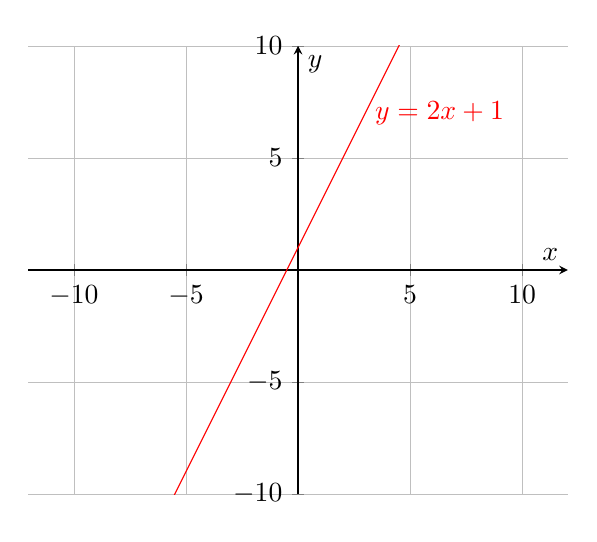
\begin{tikzpicture}
\begin{axis}[
    axis lines=middle,
    xlabel={$x$},
    ylabel={$y$},
    grid=both,
    ymin=-10, ymax=10,
    xmin=-10, xmax=10,
    grid style={line width=.1pt, draw=gray!10},
    major grid style={line width=.2pt,draw=gray!50},
    axis equal,
]
\addplot[domain=-10:10, samples=100, color=red]{2*x + 1};
\node at (axis cs:3,7) [anchor=west, color=red] {$y = 2x + 1$};
\end{axis}
\end{tikzpicture}
\caption{Graph of the linear equation \(y = 2x + 1\)}
\end{figure}

\subsubsection{Graphing Linear Inequalities}
\label{subsubsec:graphing_linear_inequalities}
Graphing linear inequalities involves shading a region of the Cartesian plane. The boundary line is drawn as either solid (for \(\leq\) or \(\geq\)) or dashed (for \(<\) or \(>\)).

% Example: Graph of y < x + 2
\begin{figure}[H]
\centering
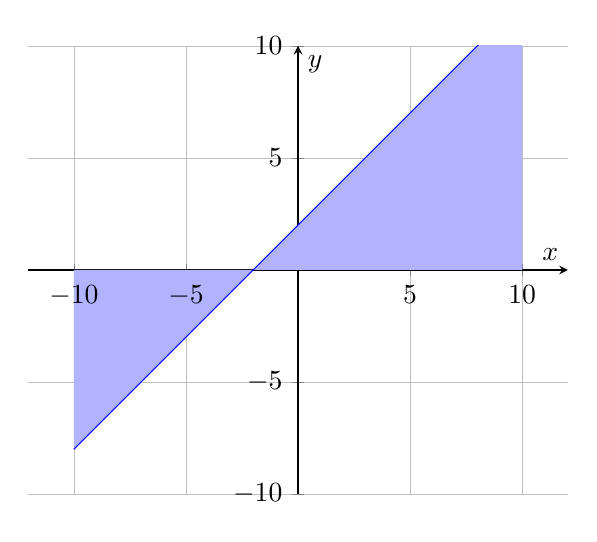
\begin{tikzpicture}
\begin{axis}[
    axis lines=middle,
    xlabel={$x$},
    ylabel={$y$},
    grid=both,
    ymin=-10, ymax=10,
    xmin=-10, xmax=10,
    grid style={line width=.1pt, draw=gray!10},
    major grid style={line width=.2pt,draw=gray!50},
    axis equal,
]
\addplot[name path=F, domain=-10:10, samples=100, color=blue]{x + 2};
\path[name path=axis] (axis cs:-10,0) -- (axis cs:10,0);
\addplot[blue!30] fill between[of=F and axis, soft clip={domain=-10:10}];
\end{axis}
\end{tikzpicture}
\caption{Graph of the linear inequality \(y < x + 2\)}
\end{figure}

\begin{exercise}
Graph the linear equation \( y = -\frac{1}{2}x + 3 \) on the Cartesian plane.
\end{exercise}

\begin{exercise}
Graph the linear inequality \( y \geq 3x - 2 \) and identify the shaded region.
\end{exercise}

% Add more examples and exercises as needed

% --- End of Graphing Linear Equations and Inequalities Section ---


% Additional Example Problems for Graphing Linear Equations and Inequalities Section

\begin{problem}
Graph the linear equation \( y = -x + 4 \) and label two points that lie on the line.
\end{problem}

\begin{solution}
To graph \( y = -x + 4 \), plot two points that satisfy the equation, such as (0,4) and (4,0), and draw a straight line through them.
\end{solution}

\begin{problem}
Graph the inequality \( y > 2x - 3 \). Indicate the region that satisfies the inequality.
\end{problem}

\begin{solution}
First, graph the line \( y = 2x - 3 \) with a dashed line since the inequality is strict (\(>\)). Then, shade the region above the line, as it represents \( y > 2x - 3 \).
\end{solution}

\begin{problem}
Determine whether the point (3, -2) lies on the graph of the equation \( 2y = 4x - 6 \).
\end{problem}

\begin{solution}
Substitute \( x = 3 \) and \( y = -2 \) into the equation. If the equation holds true, the point lies on the graph. 
\[ 2(-2) = 4(3) - 6 \]
\[ -4 = 12 - 6 \]
\[ -4 = 6 \] 
This is false, so the point (3, -2) does not lie on the graph.
\end{solution}

\begin{problem}
Sketch the inequality \( y \leq -\frac{1}{2}x + 1 \) and identify the shaded region.
\end{problem}

\begin{solution}
Graph the line \( y = -\frac{1}{2}x + 1 \) with a solid line (since the inequality includes \(\leq\)). Shade the area below the line to represent \( y \leq -\frac{1}{2}x + 1 \).
\end{solution}

% Add more problems as needed

% --- End of Additional Example Problems Section ---

\subsection{Slope of a Curve}
\label{subsec:slope_of_a_curve}
The concept of the slope of a curve at a point is fundamental in calculus. It involves finding the slope of the tangent line to the curve at that point. This concept is a precursor to derivatives, which are essentially the slope of a curve at a given point.

\subsubsection{Tangent to a Curve}
A tangent to a curve at a given point is a straight line that touches the curve at that point without crossing it. The slope of this tangent line represents the rate of change of the curve at that point.

% Example: Slope of a curve at a point
\begin{figure}[H]
\centering
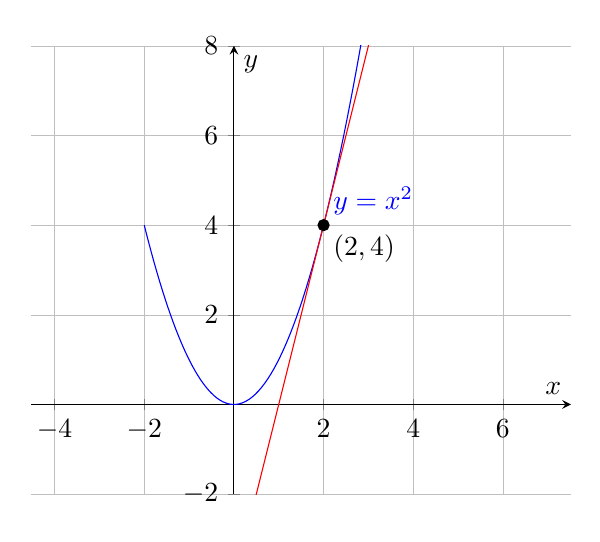
\begin{tikzpicture}
\begin{axis}[
    axis lines=middle,
    xlabel={$x$},
    ylabel={$y$},
    ymin=-2, ymax=8,
    xmin=-2, xmax=5,
    grid=both,
    grid style={line width=.1pt, draw=gray!10},
    major grid style={line width=.2pt,draw=gray!50},
    axis equal,
]

% Curve: y=x^2
\addplot[domain=-2:5, samples=100, color=blue]{x^2};
\node at (axis cs:2,4) [anchor=south west, color=blue] {$y = x^2$};

% Tangent line at x=2
\addplot[domain=0:4, samples=100, color=red]{4*x - 4};
\node at (axis cs:3.5,10) [anchor=south west, color=red] {Tangent at $x=2$};

% Point of tangency
\addplot[mark=*,color=black] coordinates {(2,4)};
\node at (axis cs:2,4) [anchor=north west] {$(2,4)$};

\end{axis}
\end{tikzpicture}
\caption{Slope of the curve \(y = x^2\) at the point \(x=2\)}
\end{figure}

In this example, the curve \(y = x^2\) has a tangent line at \(x=2\). The slope of this tangent line can be calculated using the derivative of \(y = x^2\).

\begin{exercise}
Find the slope of the tangent to the curve \(y = x^2\) at \(x=2\).
\end{exercise}

\begin{solution}
The derivative of \(y = x^2\) is \(y' = 2x\). At \(x=2\), the slope is \(y' = 2(2) = 4\). Thus, the slope of the tangent at \(x=2\) is 4.
\end{solution}

% Add more examples and exercises as needed

% --- End of Slope of a Curve Section ---


% Additional Example Problems for Slope of a Curve Section

\begin{problem}
Consider the curve given by \( y = 3x^2 - 2x + 1 \). Find the slope of the tangent to the curve at \( x = 1 \).
\end{problem}

\begin{solution}
First, find the derivative of \( y = 3x^2 - 2x + 1 \) which is \( y' = 6x - 2 \). At \( x = 1 \), the slope is \( y' = 6(1) - 2 = 4 \). Thus, the slope of the tangent at \( x = 1 \) is 4.
\end{solution}

\begin{problem}
Determine the slope of the tangent line to the curve \( y = \sqrt{x} \) at the point \( x = 4 \).
\end{problem}

\begin{solution}
The derivative of \( y = \sqrt{x} \) is \( y' = \frac{1}{2\sqrt{x}} \). At \( x = 4 \), the slope is \( y' = \frac{1}{2\sqrt{4}} = \frac{1}{4} \). Therefore, the slope of the tangent at \( x = 4 \) is \( \frac{1}{4} \).
\end{solution}

\begin{problem}
Find the equation of the tangent line to the curve \( y = x^3 \) at the point where \( x = -2 \).
\end{problem}

\begin{solution}
The derivative of \( y = x^3 \) is \( y' = 3x^2 \). The slope at \( x = -2 \) is \( y' = 3(-2)^2 = 12 \). The tangent line has the equation \( y - y_1 = m(x - x_1) \), where \( m = 12 \) and \( x_1 = -2, y_1 = (-2)^3 = -8 \). Thus, the equation is \( y + 8 = 12(x + 2) \).
\end{solution}

\begin{problem}
Calculate the slope of the tangent to the curve \( y = \frac{1}{x} \) at \( x = 3 \).
\end{problem}

\begin{solution}
The derivative of \( y = \frac{1}{x} \) is \( y' = -\frac{1}{x^2} \). At \( x = 3 \), the slope is \( y' = -\frac{1}{3^2} = -\frac{1}{9} \). Hence, the slope of the tangent at \( x = 3 \) is \( -\frac{1}{9} \).
\end{solution}

% Add more problems as needed

% --- End of Additional Example Problems Section ---


\section{Basic Geometric Figures}
\label{sec:basic_geometric_figures}
Geometry, the study of shapes and figures, begins with understanding the basics: points, lines, and planes. These elements form the foundation of more complex geometric concepts.

\subsection{Points}
A point represents a location in space. It has no size, area, length, or any other dimensional attribute. In diagrams, points are usually marked with a dot.

\begin{figure}[H]
\centering

\begin{tikzpicture}
\fill (2,2) circle (2pt) node[above] {A};
\end{tikzpicture}
\caption{A point labeled A}
\end{figure}

\subsection{Lines}
A line is a straight one-dimensional figure having no thickness and extending infinitely in both directions. A line segment is a part of a line that is bounded by two distinct end points.

\begin{figure}[H]
\centering
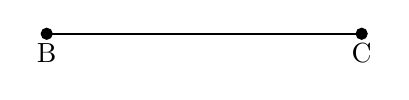
\begin{tikzpicture}
\draw[thick] (0,0) -- (4,0);
\draw[fill] (0,0) circle (2pt) node[below] {B};
\draw[fill] (4,0) circle (2pt) node[below] {C};
\end{tikzpicture}
\caption{A line segment with end points B and C}
\end{figure}

\subsection{Planes}
A plane is a flat, two-dimensional surface that extends infinitely far. Planes are usually represented by a parallelogram in diagrams.

\begin{figure}[H]
\centering
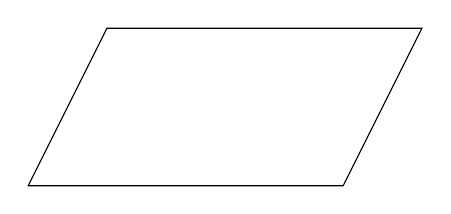
\begin{tikzpicture}
\draw (0,0) -- (4,0) -- (5,2) -- (1,2) -- cycle;
\end{tikzpicture}
\caption{Representation of a plane}
\end{figure}

\subsection{Properties of Basic Figures}
\subsubsection{Points}
Points are often used to denote a specific location or a position in space.

\subsubsection{Lines}
Lines can be characterized by their slope, which is a measure of how steep the line is. Parallel lines have the same slope, while perpendicular lines have slopes that are negative reciprocals of each other.

\subsubsection{Planes}
Planes can be defined by three non-collinear points. They are used in geometry to discuss figures like triangles, rectangles, and circles.

\begin{exercise}
Identify whether the following pairs of lines are parallel, perpendicular, or neither:
\begin{enumerate}[label=\alph*)]
\item Line 1: \( y = \frac{3}{2}x + 4 \) and Line 2: \( y = -\frac{2}{3}x + 1 \)
\item Line 3: \( y = 5x - 2 \) and Line 4: \( y = 5x + 3 \)
\end{enumerate}
\end{exercise}

\begin{solution}
\begin{enumerate}[label=\alph*)]
\item The slopes are \(\frac{3}{2}\) and \(-\frac{2}{3}\) which are negative reciprocals. So, they are perpendicular.
\item Both lines have a slope of \(5\), so they are parallel.
\end{enumerate}
\end{solution}

% Add more content and exercises as needed

% --- End of Basic Geometric Figures Section ---


% Additional Example Problems for Basic Geometric Figures Section

\begin{problem}
Consider three points \( A(1, 2) \), \( B(3, 4) \), and \( C(-1, -2) \). Determine if these points are collinear.
\end{problem}

\begin{solution}
To check for collinearity, calculate the slope of line segments \( AB \) and \( BC \). If the slopes are equal, the points are collinear. The slope of \( AB \) is \(\frac{4 - 2}{3 - 1} = 1\), and the slope of \( BC \) is \(\frac{-2 - 4}{-1 - 3} = 1\). Since the slopes are equal, points \( A \), \( B \), and \( C \) are collinear.
\end{solution}

\begin{problem}
Find the midpoint of the line segment connecting points \( D(4, -6) \) and \( E(-2, 8) \).
\end{problem}

\begin{solution}
The midpoint \( M \) has coordinates \(\left( \frac{x_1 + x_2}{2}, \frac{y_1 + y_2}{2} \right)\). Thus, \( M = \left( \frac{4 - 2}{2}, \frac{-6 + 8}{2} \right) = (1, 1)\).
\end{solution}

\begin{problem}
Given a line with the equation \( y = -3x + 7 \), determine the y-intercept and one other point on the line.
\end{problem}

\begin{solution}
The y-intercept is the point where \( x = 0 \), which is \( (0, 7) \). For another point, choose any \( x \) value, say \( x = 2 \), and calculate \( y \): \( y = -3(2) + 7 = 1 \). So, another point is \( (2, 1) \).
\end{solution}

\begin{problem}
A plane is defined by points \( F(1, 2, 3) \), \( G(4, 5, 6) \), and \( H(-2, -1, 0) \). Write the equation of the plane.
\end{problem}

\begin{solution}
To find the equation of the plane, use the formula \( Ax + By + Cz + D = 0 \), where \( A, B, C \) are the components of the normal vector to the plane, and \( D \) is a constant. This requires more advanced techniques involving vectors and cross products and is beyond the scope of basic geometry.
\end{solution}

% Add more problems as needed

% --- End of Additional Example Problems Section ---

\subsection{Points and Lines - Detail}
\label{subsec:points_and_lines_detail}
Understanding points and lines is crucial in geometry. Here, we explore their definitions and how they are represented on the Cartesian plane.

\subsubsection{Points}
A point is a fundamental concept in geometry. It represents a precise location or place in a two-dimensional space. A point has no size, shape, or real dimension.

\begin{figure}[H]
\centering

\begin{tikzpicture}
\fill (2,2) circle (2pt) node[above] {P};
\end{tikzpicture}
\caption{Representation of a point P}
\end{figure}

\subsubsection{Lines}
A line is an infinitely long, one-dimensional figure with no thickness. It extends in two opposite directions without end. Lines are often described by a linear equation in various forms such as slope-intercept form, point-slope form, or standard form.

\begin{figure}[H]
\centering
\begin{tikzpicture}
\draw[thin, ->] (-3,0) -- (3,0) node[right] {Line};
\end{tikzpicture}
\caption{Representation of a line}
\end{figure}

\subsubsection{Line Segments}
A line segment is a part of a line that is bounded by two distinct endpoints. It has a fixed length.

\begin{figure}[H]
\centering
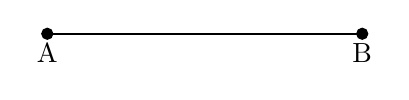
\begin{tikzpicture}
\draw[thick] (0,0) -- (4,0);
\filldraw [black] (0,0) circle (2pt) node[below] {A};
\filldraw [black] (4,0) circle (2pt) node[below] {B};
\end{tikzpicture}
\caption{A line segment AB}
\end{figure}

\subsubsection{Rays}
A ray starts at a point and extends infinitely in one direction. It is represented by a starting point and another point through which it passes.

\begin{figure}[H]
\centering
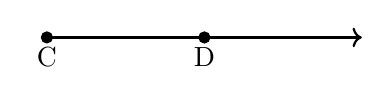
\begin{tikzpicture}
\draw[thick, ->] (0,0) -- (4,0);
\filldraw [black] (0,0) circle (2pt) node[below] {C};
\draw[fill] (2,0) circle (2pt) node[below] {D};
\end{tikzpicture}
\caption{A ray CD}
\end{figure}

% Add explanations on Cartesian Plane representation

\begin{exercise}
On the Cartesian plane, plot the points A(2, 3) and B(-1, -2). Then, draw the line segment AB.
\end{exercise}

\begin{exercise}
Describe how a ray differentiates from a line segment and draw an example of a ray on a Cartesian plane.
\end{exercise}

% --- End of Points and Lines - Detail Section ---


% Additional Example Problems for Points and Lines - Detail Section

\begin{problem}
Given two points \( P(1, 2) \) and \( Q(4, 6) \), draw the line segment \( PQ \) and calculate its length.
\end{problem}

\begin{solution}
The line segment \( PQ \) can be drawn by plotting the points \( P(1, 2) \) and \( Q(4, 6) \) on a Cartesian plane and connecting them with a straight line. The length of the line segment is found using the distance formula: 
\[ PQ = \sqrt{(4 - 1)^2 + (6 - 2)^2} = \sqrt{9 + 16} = \sqrt{25} = 5 \]
\end{solution}

\begin{problem}
On a Cartesian plane, plot the ray that starts at \( R(0, 0) \) and passes through \( S(3, 3) \). Indicate the direction of the ray.
\end{problem}

\begin{solution}
Plot the point \( R(0, 0) \) and draw a line passing through \( S(3, 3) \) extending infinitely in the direction away from \( R \). The direction of the ray is towards the upper right quadrant.
\end{solution}

\begin{problem}
If the line segment \( AB \) has endpoint \( A(2, 3) \) and midpoint \( M(5, 7) \), find the coordinates of endpoint \( B \).
\end{problem}

\begin{solution}
Using the midpoint formula, where \( M \) is the midpoint of \( AB \): \( M = \left( \frac{x_A + x_B}{2}, \frac{y_A + y_B}{2} \right) \), we have \( 5 = \frac{2 + x_B}{2} \) and \( 7 = \frac{3 + y_B}{2} \). Solving for \( x_B \) and \( y_B \), we get \( x_B = 8 \) and \( y_B = 11 \). So, \( B(8, 11) \).
\end{solution}

\begin{problem}
Create a diagram showing a point \( T \) and two rays \( TA \) and \( TB \) such that \( \angle ATB \) is a right angle.
\end{problem}

\begin{solution}
This problem requires drawing a point \( T \) and two rays \( TA \) and \( TB \) that form a right angle at point \( T \). The rays can be drawn on a Cartesian plane with \( TA \) and \( TB \) perpendicular to each other.
\end{solution}

% Add more problems as needed

% --- End of Additional Example Problems Section ---

\subsection{Vectors in Geometry}
\label{subsec:vectors_in_geometry}

In geometry and calculus, vectors are essential mathematical objects that have both magnitude and direction. They are used to represent various physical quantities such as displacement, velocity, and force. Vectors are represented as arrows in a coordinate system, where the length of the arrow represents the magnitude of the vector, and the direction of the arrow represents the direction of the vector.

\subsection{Vector Representation}

A vector in a two-dimensional space can be represented as:

\[
\vec{v} = \begin{bmatrix}
v_x \\
v_y
\end{bmatrix}
\]

Here, $\vec{v}$ is the vector, $v_x$ is its horizontal component, and $v_y$ is its vertical component. The magnitude of the vector can be calculated using the Pythagorean theorem:

\[
|\vec{v}| = \sqrt{v_x^2 + v_y^2}
\]

In three-dimensional space, a vector can be represented as:

\[
\vec{v} = \begin{bmatrix}
v_x \\
v_y \\
v_z
\end{bmatrix}
\]

The magnitude of a three-dimensional vector is calculated similarly:

\[
|\vec{v}| = \sqrt{v_x^2 + v_y^2 + v_z^2}
\]

\subsection{Vector Operations}

Vectors can be added and subtracted component-wise. For example, to add two vectors $\vec{v}$ and $\vec{w}$:

\[
\vec{v} + \vec{w} = \begin{bmatrix}
v_x + w_x \\
v_y + w_y
\end{bmatrix}
\]

The dot product of two vectors $\vec{v}$ and $\vec{w}$ is given by:

\[
\vec{v} \cdot \vec{w} = v_x \cdot w_x + v_y \cdot w_y
\]

And the cross product of two vectors $\vec{v}$ and $\vec{w}$ in three-dimensional space is:

\[
\vec{v} \times \vec{w} = \begin{bmatrix}
v_y \cdot w_z - v_z \cdot w_y \\
v_z \cdot w_x - v_x \cdot w_z \\
v_x \cdot w_y - v_y \cdot w_x
\end{bmatrix}
\]

\subsection{Visual Representation}

Let's visualize a vector $\vec{v}$ in two dimensions using TikZ:

\begin{figure}[H]
    \centering
    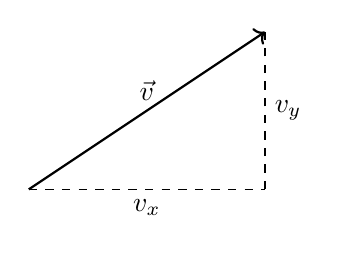
\begin{tikzpicture}
        \draw[->, thick] (0,0) -- (3,2) node[midway, above] {$\vec{v}$};
        \draw[dashed] (0,0) -- (3,0);
        \draw[dashed] (3,0) -- (3,2);
        \node[below] at (1.5,0) {$v_x$};
        \node[right] at (3,1) {$v_y$};
    \end{tikzpicture}
    \caption{Representation of vector $\vec{v}$ in two dimensions.}
    \label{fig:vector_representation}
\end{figure}

In Figure~\ref{fig:vector_representation}, we have a vector $\vec{v}$ with horizontal component $v_x$ and vertical component $v_y$.

\subsection{Significance in Geometry and Calculus}

Vectors play a crucial role in various mathematical and scientific fields. In geometry, they are used to describe lines, planes, and angles. In calculus, vectors are used to define derivatives and integrals of vector-valued functions. They are also fundamental in physics for modeling physical quantities and analyzing motion.

Understanding vectors is essential for tackling problems in fields like mechanics, electromagnetism, and computer graphics, where vector operations and geometric concepts are prevalent.

In the upcoming sections, we will explore vector algebra, vector calculus, and their applications in greater detail.

\subsection{Matrices in Geometry}
\label{subsec:matrices_in_geometry}

Matrices are fundamental mathematical objects that play a crucial role in various fields, including geometry and calculus. In this section, we will introduce the concept of matrices, their representation, and their significance in geometry and calculus.

\subsection{Matrix Representation}

A matrix is a rectangular array of numbers or symbols arranged in rows and columns. In general, a matrix $A$ is represented as:

\[
A = \begin{bmatrix}
a_{11} & a_{12} & \cdots & a_{1n} \\
a_{21} & a_{22} & \cdots & a_{2n} \\
\vdots & \vdots & \ddots & \vdots \\
a_{m1} & a_{m2} & \cdots & a_{mn}
\end{bmatrix}
\]

Here, $a_{ij}$ represents the element in the $i$-th row and $j$-th column of the matrix. The size of the matrix is determined by the number of rows ($m$) and columns ($n$).

\subsection{Matrix Operations}

Matrices support various operations, including addition, subtraction, and scalar multiplication. Matrix addition and subtraction are performed element-wise. For example, given two matrices $A$ and $B$ of the same size:

\[
C = A + B = \begin{bmatrix}
a_{11}+b_{11} & a_{12}+b_{12} & \cdots & a_{1n}+b_{1n} \\
a_{21}+b_{21} & a_{22}+b_{22} & \cdots & a_{2n}+b_{2n} \\
\vdots & \vdots & \ddots & \vdots \\
a_{m1}+b_{m1} & a_{m2}+b_{m2} & \cdots & a_{mn}+b_{mn}
\end{bmatrix}
\]

Scalar multiplication involves multiplying each element of the matrix by a scalar value. For example, if $c$ is a scalar:

\[
D = cA = \begin{bmatrix}
ca_{11} & ca_{12} & \cdots & ca_{1n} \\
ca_{21} & ca_{22} & \cdots & ca_{2n} \\
\vdots & \vdots & \ddots & \vdots \\
ca_{m1} & ca_{m2} & \cdots & ca_{mn}
\end{bmatrix}
\]

\subsection{Visual Representation}

Let's visualize a matrix using TikZ:

\begin{figure}[H]
    \centering
    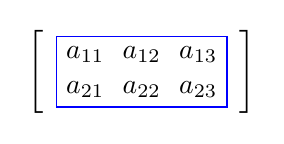
\begin{tikzpicture}
        \matrix (m) [matrix of math nodes, nodes in empty cells,
            left delimiter={[},right delimiter={]}]
        {
            a_{11} & a_{12} & a_{13} \\
            a_{21} & a_{22} & a_{23} \\
        };
        \draw[color=blue] (m-1-1.north west) -- (m-1-3.north east)
              -- (m-2-3.south east) -- (m-2-1.south west) -- cycle;
    \end{tikzpicture}
    \caption{Representation of a matrix $2 \times 3$.}
    \label{fig:matrix_representation}
\end{figure}

In Figure~\ref{fig:matrix_representation}, we have a matrix with two rows and three columns.

\subsection{Significance in Geometry and Calculus}

Matrices are used extensively in geometry and calculus to represent and manipulate geometric transformations. For example, in 2D and 3D transformations, matrices are used to perform translations, rotations, scaling, and shearing operations.

In calculus, matrices are employed in the study of multivariable functions and linear transformations. They are used to represent systems of linear equations, and matrix calculus plays a crucial role in optimization and differential equations.

Understanding matrices is essential for solving complex problems in computer graphics, engineering, physics, and many other fields where linear algebraic operations are prevalent.

In an upcoming chapter, we will further explore matrix algebra and matrix algebra applications in greater detail.

\subsection{Angles and Their Types}
\label{subsec:angles_and_their_types}

In this section, we will define angles, discuss different types of angles, and their measurement in degrees and radians. We will also provide an expanded section on radians.

\subsection{Angles}

An angle is a geometric figure formed by two rays with a common endpoint called the vertex. Angles are often measured in degrees or radians and play a fundamental role in geometry and trigonometry.

\begin{figure}[H]
    \centering
    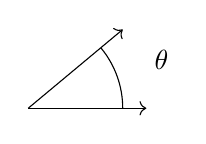
\begin{tikzpicture}
        \coordinate (O) at (0,0);
        \coordinate (A) at (1.5,0);
        \coordinate (B) at (1.2,1);
        \draw[->] (O) -- (A);
        \draw[->] (O) -- (B);
        \draw pic[draw,angle radius=1.2cm,"$\theta$",angle eccentricity=1.5] {angle=A--O--B};
    \end{tikzpicture}
    \caption{An angle $\theta$ formed by two rays.}
    \label{fig:angle_definition}
\end{figure}

\subsection{Types of Angles}

There are several types of angles based on their measurement:

\begin{itemize}
    \item \textbf{Acute Angle:} An acute angle is an angle whose measure is less than 90 degrees.
    
    \item \textbf{Obtuse Angle:} An obtuse angle is an angle whose measure is greater than 90 degrees but less than 180 degrees.
    
    \item \textbf{Right Angle:} A right angle is an angle whose measure is exactly 90 degrees. It is often denoted as $\ang{90}$.
    
    \item \textbf{Straight Angle:} A straight angle is an angle whose measure is exactly 180 degrees. It forms a straight line.
    
    \item \textbf{Reflex Angle:} A reflex angle is an angle whose measure is greater than 180 degrees but less than 360 degrees.
\end{itemize}


\begin{figure}[htbp]
    \centering
    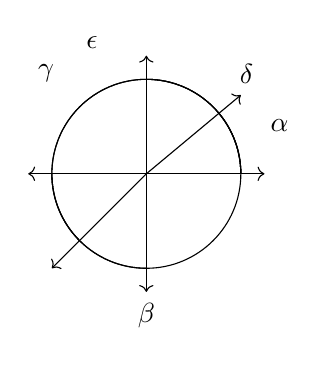
\begin{tikzpicture}
        \coordinate (O) at (0,0);
        \coordinate (A) at (1.5,0);
        \coordinate (B) at (1.2,1);
        
        % Acute Angle
        \draw[->] (O) -- (A);
        \draw[->] (O) -- (B);
        \draw pic[draw,angle radius=1.2cm,"$\alpha$",angle eccentricity=1.5] {angle=A--O--B};
        
        % Obtuse Angle
        \coordinate (C) at (-1.5,0);
        \draw[->] (O) -- (C);
        \draw pic[draw,angle radius=1.2cm,"$\beta$",angle eccentricity=1.5] {angle=C--O--A};
        
        % Right Angle
        \coordinate (D) at (0,-1.5);
        \draw[->] (O) -- (D);
        \draw pic[draw,angle radius=1.2cm,"$\gamma$",angle eccentricity=1.5] {angle=A--O--D};
        
        % Straight Angle
        \coordinate (E) at (0,1.5);
        \draw[->] (O) -- (E);
        \draw pic[draw,angle radius=1.2cm,"$\delta$",angle eccentricity=1.5] {angle=A--O--E};
        
        % Reflex Angle
        \coordinate (F) at (-1.2,-1.2);
        \draw[->] (O) -- (F);
        \draw pic[draw,angle radius=1.2cm,"$\epsilon$",angle eccentricity=1.5] {angle=A--O--F};
    \end{tikzpicture}
    \caption{Types of angles: acute ($\alpha$), obtuse ($\beta$), right ($\gamma$), straight ($\delta$), and reflex ($\epsilon$).}
    \label{fig:angle_types}
\end{figure}





\subsection{Measurement of Angles}

\paragraph{Degrees:} Degrees are a common unit of angle measurement. A full circle is divided into 360 degrees, and each degree is further divided into 60 minutes and each minute into 60 seconds.

\paragraph{Radians:} Radians are an alternative unit of angle measurement used in many mathematical and scientific applications. A full circle is equivalent to $2\pi$ radians.

\subsection{Expanded Section: Radians}

Radians are a fundamental unit for measuring angles in mathematics and physics. They offer advantages in trigonometric calculations and calculus. One radian is defined as the angle subtended at the center of a circle by an arc whose length is equal to the radius of the circle. In other words, if the arc length is equal to the radius, the angle in radians is 1 radian.





\begin{figure}[htbp]
    \centering
    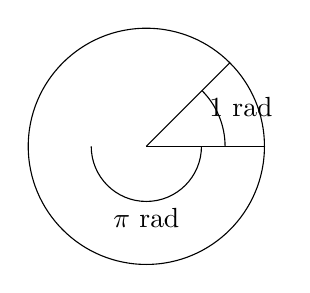
\begin{tikzpicture}
        \coordinate (O) at (0,0);
        \coordinate (A) at (1.5,0);
        \coordinate (B) at ({1.5*cos(45)},{1.5*sin(45)});
        \draw (O) circle (1.5cm);
        \draw (O) -- (A);
        \draw (O) -- (B);
        
        % Angle for 1 radian
        \draw pic[draw,angle radius=1cm,"$1$ rad",angle eccentricity=1.3] {angle=A--O--B};

        % Angle for pi radians (half circle)
        \coordinate (C) at (-1.5,0);
        \draw pic[draw,angle radius=0.7cm,"$\pi$ rad",angle eccentricity=1.3] {angle=C--O--A};
    \end{tikzpicture}
    \caption{One radian ($1$ rad) and $\pi$ radians ($\pi$ rad) in a circle.}
    \label{fig:radians_definition}
\end{figure}



In a full circle, there are $2\pi$ radians. Converting between degrees and radians is done using the formula: $\text{degrees} = \text{radians} \times \left(\frac{180}{\pi}\right)$.

\paragraph{Advantages of Radians:}

\begin{itemize}
    \item Radians simplify trigonometric calculations, especially when dealing with calculus, as they directly relate to the arc length.
    
    \item In calculus, many trigonometric derivatives and integrals are simpler when angles are measured in radians.
\end{itemize}

\subsubsection*{Practice Exercises}

1. Calculate the measure of the angle in radians when given the arc length and radius of a circle.

2. Convert angles between degrees and radians.

3. Determine the type of angle (acute, obtuse, right, etc.) given its measure.

4. Solve trigonometric equations involving angles measured in radians.

\subsubsection*{Angles and Their Types - Answer Key}
\label{subsec:angles_and_their_types_answers}

In this section, we provide solutions and explanations for the practice exercises related to angles and their types.

\begin{enumerate}
    \item \textbf{Calculate the measure of the angle in radians when given the arc length and radius of a circle.}
    
    \textbf{Solution:} To calculate the measure of the angle in radians ($\theta$) when given the arc length ($s$) and radius ($r$) of a circle, we can use the formula:
    
    \[
    \theta = \frac{s}{r}
    \]
    
    \textbf{Explanation:} This formula relates the angle in radians to the arc length and radius. By dividing the arc length by the radius, we obtain the angle in radians. Radians measure the fraction of the circumference covered by the arc.
    
    \item \textbf{Convert angles between degrees and radians.}
    
    \textbf{Solution:} To convert angles between degrees and radians, we can use the following conversion formulas:
    
    \textbf{Degrees to Radians:} To convert an angle from degrees ($\theta_{\text{deg}}$) to radians ($\theta_{\text{rad}}$), use the formula:
    
    \[
    \theta_{\text{rad}} = \frac{\theta_{\text{deg}}}{180^\circ} \pi
    \]
    
    \textbf{Radians to Degrees:} To convert an angle from radians ($\theta_{\text{rad}}$) to degrees ($\theta_{\text{deg}}$), use the formula:
    
    \[
    \theta_{\text{deg}} = \frac{\theta_{\text{rad}}}{\pi} \cdot 180^\circ
    \]
    
    \textbf{Explanation:} These conversion formulas allow us to switch between the two common units of angle measurement. To convert degrees to radians, divide by 180 and multiply by $\pi$, and to convert radians to degrees, divide by $\pi$ and multiply by 180.
    
    \item \textbf{Determine the type of angle (acute, obtuse, right, etc.) given its measure.}
    
    \textbf{Solution:} To determine the type of angle based on its measure, use the following classifications:
    
    \begin{itemize}
        \item \textbf{Acute Angle:} An angle with a measure less than 90 degrees.
        
        \item \textbf{Obtuse Angle:} An angle with a measure greater than 90 degrees but less than 180 degrees.
        
        \item \textbf{Right Angle:} An angle with a measure of exactly 90 degrees.
        
        \item \textbf{Straight Angle:} An angle with a measure of exactly 180 degrees.
        
        \item \textbf{Reflex Angle:} An angle with a measure greater than 180 degrees but less than 360 degrees.
    \end{itemize}
    
    \textbf{Explanation:} These classifications are based on the measure of the angle. Simply compare the given angle measure to these categories to determine its type.
    
    \item \textbf{Solve trigonometric equations involving angles measured in radians.}
    
    \textbf{Solution:} To solve trigonometric equations involving angles measured in radians, apply trigonometric identities and properties as needed. Solve for the unknown angle.
    
    \textbf{Explanation:} Trigonometric equations often involve angles measured in radians. Use trigonometric identities and properties to manipulate equations and isolate the unknown angle. Solve for the angle by applying inverse trigonometric functions, if necessary.
    
\end{enumerate}

In this section, we provided solutions and explanations for the practice exercises related to angles and their types. These exercises covered angle measurement, conversion between degrees and radians, angle classification, and solving trigonometric equations involving radians.

\subsubsection*{Summary}

In this section, we defined angles, discussed various types of angles, and explored their measurement in degrees and radians. Radians were highlighted for their importance in mathematics and science, particularly in trigonometry and calculus. Understanding angles and their measurement units is essential for various mathematical and scientific applications.

\subsection{Planes and Space}
\label{subsec:planes_and_space}

The concept of a plane in geometry is fundamental to understanding spatial relationships and structures. A plane is a flat, two-dimensional surface that extends infinitely in all directions. In three-dimensional space, a plane can be defined in several ways, including by a point and a normal vector, or by three non-collinear points.

\subsection{Points in Space}
A point in three-dimensional space can be defined by its coordinates \((x, y, z)\).

\subsection{Lines in Space}
A line in space can be represented by a linear equation or vector equation.

\subsection{Planes in Space}
A plane can be defined by the equation \(ax + by + cz = d\), where \(a, b, c,\) and \(d\) are constants, and \(x, y,\) and \(z\) are variables representing points on the plane.

\subsection{Visual Representation of Planes in 3D}
To visualize these concepts, we use TikZ to draw a simple representation of a 3D coordinate system with a plane.

% 3D Plane Visualization
\begin{center}
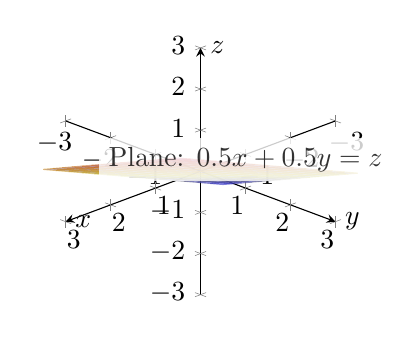
\begin{tikzpicture}
  \begin{axis}[
    view={135}{30},
    axis lines=center,
    xlabel={$x$},
    ylabel={$y$},
    zlabel={$z$},
    xmax=3, ymax=3, zmax=3,
    xmin=-3, ymin=-3, zmin=-3,
    xtick={-3,...,3},
    ytick={-3,...,3},
    ztick={-3,...,3},
    every axis x label/.style={at={(ticklabel* cs:1)},anchor=west},
    every axis y label/.style={at={(ticklabel* cs:1)},anchor=west},
    every axis z label/.style={at={(ticklabel* cs:1)},anchor=west}
  ]
  
  % Draw plane
  \addplot3[
    surf,
    opacity=0.5,
    domain=-2:2,
    domain y=-1.5:1.5,
    samples=15,
    samples y=15,
    fill=blue!50,
  ] 
  {0.5*x + 0.5*y};

  % Label plane
  \node[fill=white, opacity=0.8] at (axis cs: 1,2,1.5) {Plane: \(0.5x + 0.5y = z\)};

  \end{axis}
\end{tikzpicture}
\end{center}

This diagram represents a simple plane in a three-dimensional coordinate system. By studying these basic elements, we can begin to understand more complex geometric structures and their properties in space.

\begin{exercise}
  Consider a plane defined by the equation \(2x - y + 3z = 6\). Identify a point that lies on this plane.
\end{exercise}

\begin{exercise}
  Find the equation of a plane passing through the points \( (1, 2, 3) \), \( (2, -1, 4) \), and \( (0, -1, 2) \).
\end{exercise}


\subsubsection*{Solutions to Exercises on Planes and Space}

\begin{solution}[Exercise 1]
To find a point that lies on the plane defined by \(2x - y + 3z = 6\), we can choose arbitrary values for two of the variables and solve for the third. 

For instance, let's choose \(x = 1\) and \(y = 2\). Substituting these into the plane equation, we get:
\[ 2(1) - 2 + 3z = 6 \]
\[ 2 - 2 + 3z = 6 \]
\[ 3z = 6 \]
\[ z = 2 \]

Thus, the point \((1, 2, 2)\) lies on the plane.
\end{solution}

\begin{solution}[Exercise 2]
To find the equation of the plane passing through the points \( (1, 2, 3) \), \( (2, -1, 4) \), and \( (0, -1, 2) \), we first find two vectors that lie on the plane by subtracting coordinates:

Vector \(\mathbf{AB} = (2 - 1, -1 - 2, 4 - 3) = (1, -3, 1)\) \\
Vector \(\mathbf{AC} = (0 - 1, -1 - 2, 2 - 3) = (-1, -3, -1)\)

Next, we find the normal vector \(\mathbf{n}\) to the plane by taking the cross product of \(\mathbf{AB}\) and \(\mathbf{AC}\):
\[ \mathbf{n} = \mathbf{AB} \times \mathbf{AC} \]
\[ = \begin{vmatrix} \mathbf{i} & \mathbf{j} & \mathbf{k} \\ 1 & -3 & 1 \\ -1 & -3 & -1 \end{vmatrix} \]
\[ = \mathbf{i}(-3 \cdot -1 - (-3) \cdot 1) - \mathbf{j}(1 \cdot -1 - (-1) \cdot 1) + \mathbf{k}(1 \cdot -3 - (-3) \cdot -1) \]
\[ = 0\mathbf{i} + 0\mathbf{j} - 6\mathbf{k} \]
\[ \mathbf{n} = (0, 0, -6) \]

Since the normal vector is parallel to the \(z\)-axis, the plane is parallel to the \(xy\)-plane. The equation of the plane can thus be written as \( z = k \) for some constant \( k \). To find \( k \), we substitute the coordinates of any of the given points, say \( (1, 2, 3) \):
\[ z = 3 \]

Therefore, the equation of the plane is \( z = 3 \).
\end{solution}


% HERE

\section{Triangles and Congruence}
\label{sec:triangles_and_congruence}

Triangles are fundamental geometric shapes that play a crucial role in various mathematical and practical contexts. In this section, we explore different types of triangles, discuss the concept of congruence, and highlight the significance of triangles in geometry.

\subsection{Types of Triangles}

Triangles can be classified into several types based on their sides and angles:

Based on Sides
\begin{comment}
\begin{enumerate}
    \item \textbf{Equilateral Triangle:} All three sides are of equal length. Each angle measures $60^\circ$. (See Figure \ref{fig:equilateral_triangle})
    
    \begin{figure}[H]
        \centering
        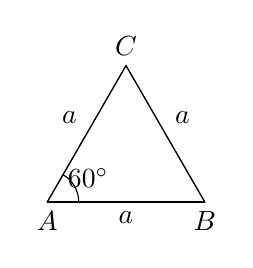
\begin{tikzpicture}
            \coordinate (A) at (0,0);
            \coordinate (B) at (2,0);
            \coordinate (C) at (1,{sqrt(3)});
            
            \draw (A) -- (B) -- (C) -- cycle;
            
            \node[below] at (A) {$A$};
            \node[below] at (B) {$B$};
            \node[above] at (C) {$C$};
            
            \draw (A) -- node[above left] {$a$} (C);
            \draw (B) -- node[above right] {$a$} (C);
            \draw (A) -- node[below] {$a$} (B);
            
            \draw pic[draw,angle radius=0.4cm,"$60^\circ$",angle eccentricity=1.5] {angle=B--A--C};
        \end{tikzpicture}
        \caption{Equilateral Triangle}
        \label{fig:equilateral_triangle}
    \end{figure}
    
    \item \textbf{Isosceles Triangle:} Two sides are of equal length, and the angles opposite those sides are congruent. The third side may have a different length. (See Figure \ref{fig:isosceles_triangle})
    
    \begin{figure}[H]
        \centering
        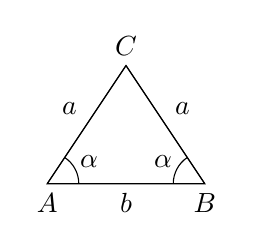
\begin{tikzpicture}
            \coordinate (A) at (0,0);
            \coordinate (B) at (2,0);
            \coordinate (C) at (1,1.5);
            
            \draw (A) -- (B) -- (C) -- cycle;
            
            \node[below] at (A) {$A$};
            \node[below] at (B) {$B$};
            \node[above] at (C) {$C$};
            
            \draw (A) -- node[above left] {$a$} (C);
            \draw (B) -- node[above right] {$a$} (C);
            \draw (A) -- node[below] {$b$} (B);
            
            \draw pic[draw,angle radius=0.4cm,"$\alpha$",angle eccentricity=1.5] {angle=B--A--C};
            \draw pic[draw,angle radius=0.4cm,"$\alpha$",angle eccentricity=1.5] {angle=C--B--A};
        \end{tikzpicture}
        \caption{Isosceles Triangle}
        \label{fig:isosceles_triangle}
    \end{figure}
    
    \item \textbf{Scalene Triangle:} All three sides have different lengths, and all three angles are distinct. (See Figure \ref{fig:scalene_triangle})
    
    \begin{figure}[H]
        \centering
        \begin{tikzpicture}
            \coordinate (A) at (0,0);
            \coordinate (B) at (2,0);
            \coordinate (C) at (1,1.2);
            
            \draw (A) -- (B) -- (C) -- cycle;
            
            \node[below] at (A) {$A$};
            \node[below] at (B) {$B$};
            \node[above] at (C) {$C$};
            
            \draw (A) -- node[above left] {$a$} (C);
            \draw (B) -- node[above right] {$b$} (C);
            \draw (A) -- node[below] {$c$} (B);
            
            \draw pic[draw,angle radius=0.4cm,"$\alpha$",angle eccentricity=1.5] {angle=B--A--C};
            \draw pic[draw,angle radius=0.4cm,"$\beta$",angle eccentricity=1.5] {angle=C--B--A};
            \draw pic[draw,angle radius=0.4cm,"$\gamma$",angle eccentricity=1.5] {angle=A--C--B};
        </tikzpicture}
        \caption{Scalene Triangle}
        \label{fig:scalene_triangle}
    \end{figure}
\end{enumerate}

\end{comment}
Based on Angles

\begin{comment}
\begin{enumerate}
    \item \textbf{Acute Triangle:} All three angles are acute (less than $90^\circ$). (See Figure \ref{fig:acute_triangle})
    
    \begin{figure}[H]
        \centering
        \begin{tikzpicture}
            \coordinate (A) at (0,0);
            \coordinate (B) at (2,0);
            \coordinate (C) at (1,1.5);
            
            \draw (A) -- (B) -- (C) -- cycle;
            
            \node[below] at (A) {$A$};
            \node[below] at (B) {$B$};
            \node[above] at (C) {$C$};
            
            \draw (A) -- node[above left] {$a$} (C);
            \draw (B) -- node[above right] {$b$} (C);
            \draw (A) -- node[below] {$c$} (B);
            
            \draw pic[draw,angle radius=0.4cm,"$\alpha$",angle eccentricity=1.5] {angle=B--A--C};
            \draw pic[draw,angle radius=0.4cm,"$\beta$",angle eccentricity=1.5] {angle=C--B--A};
            \draw pic[draw,angle radius=0.4cm,"$\gamma$",angle eccentricity=1.5] {angle=A--C--B};
        \end{tikzpicture}
        \caption{Acute Triangle}
        \label{fig:acute_triangle}
    \end{figure}
    
    \item \textbf{Obtuse Triangle:} One angle is obtuse (greater than $90^\circ$). (See Figure \ref{fig:obtuse_triangle})
    
    \begin{figure}[H]
        \centering
        \begin{tikzpicture}
            \coordinate (A) at (0,0);
            \coordinate (B) at (2,0);
            \coordinate (C) at (1,1.2);
            
            \draw (A) -- (B) -- (C) -- cycle;
            
            \node[below] at (A) {$A$};
            \node[below] at (B) {$B$};
            \node[above] at (C) {$C$};
            
            \draw (A) -- node[above left] {$a$} (C);
            \draw (B) -- node[above right] {$b$} (C);
            \draw (A) -- node[below] {$c$} (B);
            
            \draw pic[draw,angle radius=0.4cm,"$\alpha$",angle eccentricity=1.5] {angle=B--A--C};
            \draw pic[draw,angle radius=0.4cm,"$\beta$",angle eccentricity=1.5] {angle=C--B--A};
            \draw pic[draw,angle radius=0.4cm,"$\gamma$",angle eccentricity=1.5] {angle=A--C--B};
        </tikzpicture}
        \caption{Obtuse Triangle}
        \label{fig:obtuse_triangle}
    \end{figure}
    
    \item \textbf{Right Triangle:} One angle is a right angle ($90^\circ$). (See Figure \ref{fig:right_triangle})
    
    \begin{figure}[H]
        \centering
        \begin{tikzpicture}
            \coordinate (A) at (0,0);
            \coordinate (B) at (2,0);
            \coordinate (C) at (0,1.5);
            
            \draw (A) -- (B) -- (C) -- cycle;
            
            \node[below] at (A) {$A$};
            \node[below] at (B) {$B$};
            \node[left] at (C) {$C$};
            
            \draw (A) -- node[above left] {$a$} (C);
            \draw (B) -- node[above right] {$b$} (C);
            \draw (A) -- node[below] {$c$} (B);
            
            \draw pic[draw,angle radius=0.4cm,"$\alpha$",angle eccentricity=1.5] {angle=B--A--C};
            \draw pic[draw,angle radius=0.4cm,"$\beta$",angle eccentricity=1.5] {angle=C--B--A};
            \draw pic[draw,angle radius=0.4cm,"$90^\circ$",angle eccentricity=1.5] {angle=A--C--B};
        \end{tikzpicture}
        \caption{Right Triangle}
        \label{fig:right_triangle}
    \end{figure}
\end{enumerate}
\end{comment}
\subsection{Congruence of Triangles}

Congruence is a fundamental concept in geometry that deals with the equality of shapes and sizes. Two triangles are considered congruent if their corresponding sides and angles are equal. Several congruence criteria can be used to determine the congruence of triangles, including Side-Angle-Side (SAS), Side-Side-Side (SSS), Angle-Side-Angle (ASA), and more.

SAS Congruence Criterion

Two triangles are congruent if two sides and the included angle of one triangle are equal to the corresponding two sides and the included angle of the other triangle.

SSS Congruence Criterion

Two triangles are congruent if all three sides of one triangle are equal to the corresponding three sides of the other triangle.

ASA Congruence Criterion

Two triangles are congruent if two angles and the included side of one triangle are equal to the corresponding two angles and the included side of the other triangle.

\subsection{Applications of Triangles}

Triangles have practical applications in various fields, including architecture, engineering, and trigonometry. Here are some examples:

Architecture and Construction

Architects use triangular principles to design stable structures. Triangles are often found in the construction of roofs and trusses, which distribute weight evenly and prevent collapsing.

Engineering

In engineering, triangles are essential for analyzing forces and constructing stable frameworks. The study of statics and structural analysis relies heavily on triangular calculations.

Trigonometry

Trigonometry, the study of the relationships between angles and sides of triangles, is a crucial branch of mathematics used in fields like navigation, physics, and computer graphics.

In the upcoming sections, we will delve deeper into congruence criteria, triangle inequalities, and practical applications of triangles in various fields.

Conclusion

Triangles are fundamental geometric shapes with diverse properties and applications. Understanding the types of triangles and the concept of congruence is essential for solving geometric problems and real-world applications.


\subsection{Types of Triangles Again}
\label{subsec:types_of_triangles}
Discuss different types of triangles based on sides (equilateral, isosceles, scalene) and angles (acute, right, obtuse).


\subsection{Congruence and Similarity Again}
\label{subsec:congruence_and_similarity}
Define congruence and similarity in the context of triangles, including criteria like SSS, SAS, ASA, and RHS.

\subsection{Trigonometric Ratios in Right Triangles}
\label{subsec:trigonometric_ratios}
Introduce the concept of trigonometric ratios in right triangles and their importance in both geometry and calculus.


\section{Right Triangles and the Pythagorean Theorem}
\label{sec:right_triangles_pythagorean}
Right triangles form the basis of trigonometry, which is integral to calculus.


\subsection{Properties of Right Triangles}
\label{subsec:properties_right_triangles}
Discussion on right triangles, including the definitions and properties specific to them.


\subsection{The Pythagorean Theorem}
\label{subsec:pythagorean_theorem}
The Pythagorean theorem states that in a right triangle, the square of the length of the hypotenuse is equal to the sum of the squares of the other two sides.


\subsubsection{Graphical Interpretation of the Pythagorean Theorem}
\label{subsubsec:graphical_pythagorean}
Provide a visual interpretation of the Pythagorean theorem, possibly including a TikZ diagram to illustrate the concept.


\subsection{Trigonometric Identities}
\label{subsec:trigonometric_identities}
Introduce basic trigonometric identities and their geometric interpretations, linking to their use in calculus.


\section{Understanding Area}
\label{sec:understanding_area}
The concept of area is a foundational aspect of geometry and is pivotal in integral calculus.


\subsection{Basic Principles of Area}
\label{subsec:basic_principles_area}
Discuss the fundamental principles and units of area measurement.


\subsection{Area Under a Curve}
\label{subsec:area_under_curve}
Introduce the preliminary idea of the area under a curve, connecting it to integral calculus concepts.


\section{Circle Geometry}
\label{sec:circle_geometry}
The circle is a fundamental shape in both geometry and calculus. This section covers its properties and equations.


\subsection{Properties of Circles}
\label{subsec:properties_of_circles}
Discuss the basic properties of circles, including tangents, chords, arc, and sector.


\subsection{Equation of a Circle}
\label{subsec:equation_of_a_circle}
Derive and explain the standard form and general form of the equation of a circle.


\subsection{Parametric Equations of a Circle}
\label{subsec:parametric_equations_circle}
Introduce the concept of parametric equations for a circle and their relevance in calculus.


\subsection{Area of a Circle and Pi (\(\pi\))}
\label{subsec:area_circle_pi}
Explore the relationship between the area of a circle and the mathematical constant \(\pi\). Discuss the formula \(A = \pi r^2\) and its derivation.


% Area Formulas for Common 2-D Shapes Section
\section{Area Formulas for Common 2-D Shapes}
\label{sec:area_formulas_2d}
This section will include formulas and explanations for finding the area of common two-dimensional shapes.


\subsection{Decomposing Complex Shapes}
\label{subsec:decomposing_complex_shapes}
Discuss the method of decomposing complex shapes into simpler ones to find their area. This technique is foundational for understanding the integration of irregular shapes in calculus.


\subsection{Triangles}
\label{subsec:area_triangles}
Include formulas for the area of different types of triangles (e.g., equilateral, right-angled).


\subsection{Rectangles and Squares}
\label{subsec:area_rectangles_squares}
Discuss the formulas for the area of rectangles and squares.


\subsection{Other Common Shapes}
\label{subsec:area_other_shapes}
Include area formulas for other common shapes like parallelograms, trapezoids, and ellipses.


% Volume Formulas for Common 3-D Objects Section
\section{Volume Formulas for Common 3-D Objects}
\label{sec:volume_formulas_3d}
Understanding the volume of three-dimensional objects is essential for many calculus applications.


\subsection{Cross-Sectional Area}
\label{subsec:cross_sectional_area}
Introduce the concept of cross-sectional area and its role in determining the volume of 3-D objects, paving the way for understanding volume integration in calculus.


\subsection{Prisms and Cylinders}
\label{subsec:volume_prisms_cylinders}
Discuss the formulas for finding the volume of prisms and cylinders.


\subsection{Pyramids and Cones}
\label{subsec:volume_pyramids_cones}
Include the formulas and methods to calculate the volume of pyramids and cones.


\subsection{Spheres}
\label{subsec:volume_spheres}
Provide the formula for the volume of a sphere and discuss its derivation.


% Applications in Calculus Section
\section{Applications in Calculus}
\label{sec:applications_in_calculus}
This final section highlights how geometric concepts find applications in calculus.


\subsection{Limits and Continuity}
\label{subsec:limits_and_continuity}
Discuss how geometric understanding aids in comprehending limits and continuity in calculus.


\subsection{Integrals and Area}
\label{subsec:integrals_and_area}
Explore how integration in calculus is used for finding areas under curves, with a basis in geometric understanding of area.

\subsection{Real-World Examples in Calculus}
\label{subsec:real_world_examples_calculus}
Provide real-world examples and case studies demonstrating the use of geometric concepts in various calculus applications.


\subsection{Geometric Interpretation of Derivatives and Integrals}
\label{subsec:geometric_interpretation_derivatives_integrals}
Explore the geometric interpretation of derivatives (slopes and rates of change) and integrals (area under curves) in calculus.

% General Enhancements for the Chapter
\section*{Enhancements for the Chapter}
\label{sec:enhancements_for_chapter}
% Visual Elements
\paragraph{Visual Elements}
Emphasize the inclusion of diagrams, graphs, and visual aids throughout the chapter to enhance understanding of geometric concepts.


% Exercises Bridging Geometry and Calculus
\paragraph{Bridging Exercises}
Include exercises at the end of each section designed to bridge the gap between geometric concepts and their applications in calculus, reinforcing learning and application skills.


% Concluding remarks for the chapter
\section*{Conclusion}
\label{sec:geom_conclusion}
This chapter serves as the foundation for understanding the vital role of Geometry in calculus. As you progress through your studies, these concepts will become second nature, providing the tools necessary for analyzing and solving a broad range of problems in higher mathematics.


% Ensure that the conclusion is added to the table of contents
\addcontentsline{toc}{section}{Conclusion}


% --- End of Geometry Chapter ---

\chapter{Fundamental Algebra for Calculus}
\label{chap:algebra_for_calculus}
\textit{Algebra forms the language through which we describe and solve a wide range of mathematical problems, including those in calculus. This chapter covers algebra concepts that are particularly relevant for understanding and applying calculus.}


\subsection{Basic Algebraic Operations}
\label{subsec:basic_algebraic_operations}
Basic algebraic operations are the foundation of algebra. They include addition, subtraction, multiplication, and division. Each of these operations follows specific properties crucial in simplifying and solving algebraic expressions.


\subsubsection{Addition}
Addition combines two or more numbers into a single sum. The properties of addition include:
\begin{itemize}
    \item Commutative property: \( a + b = b + a \)
    \item Associative property: \( (a + b) + c = a + (b + c) \)
    \item Identity property: \( a + 0 = a \)
\end{itemize}


\subsubsection{Subtraction}
Subtraction finds the difference between two numbers. It is the inverse operation of addition.


\subsubsection{Multiplication}
Multiplication combines a number with itself a specified number of times. Its properties are similar to addition:
\begin{itemize}
    \item Commutative property: \( ab = ba \)
    \item Associative property: \( (ab)c = a(bc) \)
    \item Identity property: \( a \cdot 1 = a \)
    \item Distributive property: \( a(b + c) = ab + ac \)
\end{itemize}


\subsubsection{Division}
Division splits a number into specified equal parts. It is the inverse operation of multiplication.


% Examples
\begin{exercise}
Calculate \( 3 + 4 \) and \( 4 + 3 \) to demonstrate the commutative property of addition.
\end{exercise}


\begin{exercise}
Show that \( 2 \times (3 + 5) = 2 \times 3 + 2 \times 5 \) using the distributive property of multiplication.
\end{exercise}


\subsubsection{Properties in Algebraic Expressions}
These properties are not only applicable to numbers but also to algebraic expressions. For example, for any variables \( x \) and \( y \), \( x + y = y + x \) and \( x(y + z) = xy + xz \).


\begin{problem}
If \( x = 2 \) and \( y = 3 \), verify \( x + y = y + x \).
\end{problem}


\begin{problem}
Simplify the expression \( 3(x + 4) \) using the distributive property.
\end{problem}


% End of Basic Algebraic Operations Section


\subsection*{Practice Problems on Basic Algebraic Operations}
\addcontentsline{toc}{subsection}{Practice Problems on Basic Algebraic Operations}


\begin{problem}
Solve the following expressions:
\begin{enumerate}[label=(\alph*)]
    \item \( 7 + 8 \)
    \item \( 15 - 4 \)
    \item \( 3 \times 5 \)
    \item \( 16 \div 4 \)
\end{enumerate}
\end{problem}


\begin{problem}
Using the commutative property of multiplication, show that \( 4 \times 7 = 7 \times 4 \).
\end{problem}


\begin{problem}
Apply the distributive property to simplify \( 5(2 + 3) \).
\end{problem}


\begin{problem}
If \( a = 4 \) and \( b = 6 \), calculate the following:
\begin{enumerate}[label=(\alph*)]
    \item \( a + b \)
    \item \( a - b \)
    \item \( ab \)
    \item \( \frac{a}{b} \), if \( b \neq 0 \)
\end{enumerate}
\end{problem}


\begin{problem}
Verify the associative property of addition with \( a = 1 \), \( b = 2 \), and \( c = 3 \) by showing that \( (a + b) + c = a + (b + c) \).
\end{problem}


\begin{exercise}
For \( x = 5 \), simplify and calculate \( 2x + 3 \).
\end{exercise}


\begin{exercise}
Demonstrate the identity property of multiplication by showing that \( 7 \times 1 = 7 \).
\end{exercise}


% End of Practice Problems Section


\subsection{Set Notation - Detail}
\label{subsec:set_notation_detail}
Set notation is a method of specifying groups of numbers through defined criteria. This section explores the representation of various sets of real numbers on the real line, particularly focusing on intervals with open and closed boundary points.


\subsubsection{Types of Intervals}
\begin{itemize}
    \item \textbf{Open Interval} \( (a, b) \): It includes all real numbers between \( a \) and \( b \) but not \( a \) and \( b \) themselves.
    \item \textbf{Closed Interval} \( [a, b] \): It includes all real numbers between \( a \) and \( b \), including \( a \) and \( b \).
    \item \textbf{Half-Open Interval} \( [a, b) \) or \( (a, b] \): It includes all real numbers between \( a \) and \( b \), including one of the endpoints.
\end{itemize}


\subsubsection{Graphical Representation of Intervals}
Using the `tikz` package, intervals can be represented on the real line.


% Example of an open interval
\begin{center}
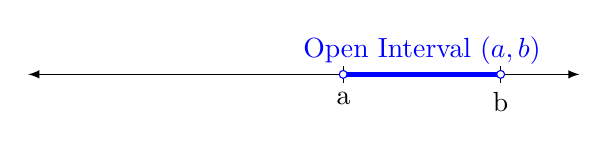
\begin{tikzpicture}
    \draw[latex-latex] (-3.5,0) -- (3.5,0); % Real line
    \draw[ultra thick, blue] (0.5,0) -- (2.5,0); % Interval line
    \draw[shift={(0.5,0)},color=black] (0pt,3pt) -- (0pt,-3pt) node[below] {a};
    \draw[shift={(2.5,0)},color=black] (0pt,3pt) -- (0pt,-3pt) node[below] {b};
    \draw[fill=white,draw=blue] (0.5,0) circle (0.05);
    \draw[fill=white,draw=blue] (2.5,0) circle (0.05);
    \node at (1.5,0.3) {\textcolor{blue}{Open Interval \( (a, b) \)}};
\end{tikzpicture}
\end{center}


% Example of a closed interval
\begin{center}
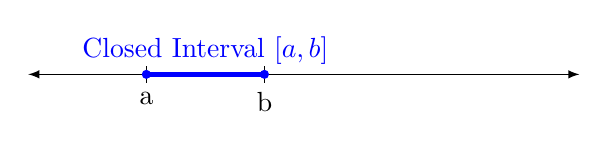
\begin{tikzpicture}
    \draw[latex-latex] (-3.5,0) -- (3.5,0); % Real line
    \draw[ultra thick, blue] (-2,0) -- (-0.5,0); % Interval line
    \draw[shift={(-2,0)},color=black] (0pt,3pt) -- (0pt,-3pt) node[below] {a};
    \draw[shift={(-0.5,0)},color=black] (0pt,3pt) -- (0pt,-3pt) node[below] {b};
    \draw[fill=blue,draw=blue] (-2,0) circle (0.05);
    \draw[fill=blue,draw=blue] (-0.5,0) circle (0.05);
    \node at (-1.25,0.3) {\textcolor{blue}{Closed Interval \( [a, b] \)}};
\end{tikzpicture}
\end{center}


\subsubsection{Set Builder Notation}
Set builder notation is another way to describe sets. For example, the set of all \( x \) such that \( x \) is greater than 2 can be written as \( \{ x \in \mathbb{R} | x > 2 \} \).


\begin{exercise}
Represent the set \( \{ x \in \mathbb{R} | -3 < x \leq 1 \} \) on the real line.
\end{exercise}


\begin{exercise}
Write the interval \( [2, 5) \) in set builder notation.
\end{exercise}


\begin{solution}
The interval \( [2, 5) \) can be written as \( \{ x \in \mathbb{R} | 2 \leq x < 5 \} \).
\end{solution}




\subsection*{Practice Problems on Set Notation and Intervals}
\addcontentsline{toc}{subsection}{Practice Problems on Set Notation and Intervals}


\begin{problem}
Graphically represent the following intervals on the real line:
\begin{enumerate}[label=(\alph*)]
    \item The open interval \( (-2, 3) \)
    \item The closed interval \( [-1, 2] \)
    \item The half-open interval \( (0, 4] \)
\end{enumerate}
\end{problem}


\begin{problem}
Write in set builder notation and represent graphically on the real line:
\begin{enumerate}[label=(\alph*)]
    \item All real numbers greater than or equal to -1.
    \item All real numbers less than 5.
    \item All real numbers between -2 and 2, including -2 but not 2.
\end{enumerate}
\end{problem}


\begin{problem}
Identify the type of interval and represent it on the real line for the following sets:
\begin{enumerate}[label=(\alph*)]
    \item \( \{ x \in \mathbb{R} | -3 \leq x < 1 \} \)
    \item \( \{ x \in \mathbb{R} | x > -2 \} \)
    \item \( \{ x \in \mathbb{R} | 0 \leq x \leq 3 \} \)
\end{enumerate}
\end{problem}


\begin{problem}
Determine if the number 0.5 is in the set \( \{ x \in \mathbb{R} | x^2 < 1 \} \). Justify your answer.
\end{problem}


\begin{problem}
For the set \( \{ x \in \mathbb{R} | x^2 - 4x + 3 = 0 \} \), find the values of \( x \) and represent the set on the real line.
\end{problem}


\begin{exercise}
Express the interval \( x < -3 \) or \( x > 3 \) graphically on the real line.
\end{exercise}


\begin{exercise}
Represent the interval \( -1 \leq x < 2 \) on the real line and write it in set builder notation.
\end{exercise}


% End of Practice Problems Section


\subsection{Types of Real Numbers}
\label{subsec:types_real_numbers}
Real numbers encompass various types, each with unique properties. Understanding these types is crucial for grasping the scope of real numbers in algebra.


\subsubsection{Natural Numbers}
Natural numbers, denoted by \( \mathbb{N} \), are the set of all positive integers starting from 1. In set notation, this is represented as \( \mathbb{N} = \{1, 2, 3, \ldots\} \).


\subsubsection{Whole Numbers}
Whole numbers include all natural numbers along with zero. They are denoted by \( \mathbb{W} \) and represented as \( \mathbb{W} = \{0, 1, 2, \ldots\} \).


\subsubsection{Integers}
Integers, denoted by \( \mathbb{Z} \), are the set of all whole numbers and their negative counterparts. They can be represented as \( \mathbb{Z} = \{\ldots, -3, -2, -1, 0, 1, 2, 3, \ldots\} \).


\subsubsection{Rational Numbers}
Rational numbers, denoted by \( \mathbb{Q} \), are numbers that can be expressed as a ratio of two integers \( \frac{a}{b} \) where \( b \neq 0 \). This set includes fractions and terminating or repeating decimals.


\subsubsection{Irrational Numbers}
Irrational numbers cannot be expressed as a simple fraction. This set includes numbers like \( \pi \) and \( \sqrt{2} \). They have non-repeating, non-terminating decimal parts.


\subsubsection{Real Number Line Representation}
Using the `tikz` package, we can represent these subsets on the real number line.


% Drawing the real number line
\begin{center}
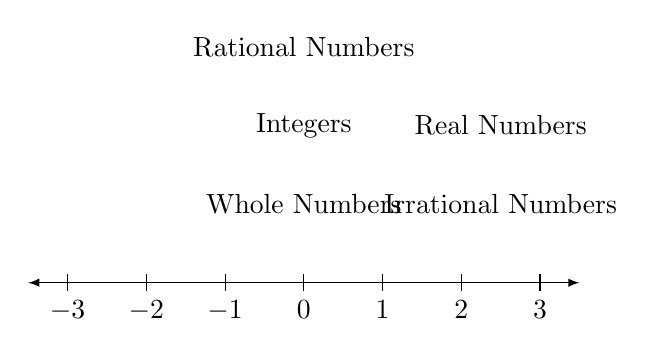
\begin{tikzpicture}
    \draw[latex-latex] (-3.5,0) -- (3.5,0); % Real number line
    \foreach \x in {-3, -2, -1, 0, 1, 2, 3} 
        \draw[shift={(\x,0)},color=black] (0pt,3pt) -- (0pt,-3pt) node[below] {$\x$};
    \node at (0,1) {Whole Numbers};
    \node at (0,2) {Integers};
    \node at (0,3) {Rational Numbers};
    \node at (2.5,1) {Irrational Numbers};
    \node at (2.5,2) {Real Numbers};
\end{tikzpicture}
\end{center}


% Exercises
\begin{exercise}
Identify whether the number \( \frac{1}{2} \) is a natural, whole, integer, or rational number.
\end{exercise}


\begin{exercise}
Is the number \( \sqrt{3} \) a rational or irrational number? Justify your answer.
\end{exercise}


% End of Types of Real Numbers Section


\subsection*{Practice Problems on Types of Real Numbers}
\addcontentsline{toc}{subsection}{Practice Problems on Types of Real Numbers}


\begin{problem}
Classify each of the following numbers as natural, whole, integer, rational, or irrational:
\begin{enumerate}[label=(\alph*)]
    \item \( 0 \)
    \item \( -3 \)
    \item \( \frac{4}{5} \)
    \item \( \sqrt{5} \)
    \item \( 7 \)
\end{enumerate}
\end{problem}


\begin{problem}
Determine if the following statements are true or false. Justify your answer:
\begin{enumerate}[label=(\alph*)]
    \item Every integer is a rational number.
    \item Every natural number is also a whole number.
    \item The number \( \pi \) is a rational number.
    \item The number \( 0.121212\ldots \) (repeating) is irrational.
\end{enumerate}
\end{problem}


\begin{problem}
Provide an example of a number that is:
\begin{enumerate}[label=(\alph*)]
    \item A rational number but not an integer.
    \item An irrational number.
    \item A whole number but not a natural number.
    \item An integer but not a whole number.
\end{enumerate}
\end{problem}


\begin{exercise}
Is the number \( \frac{1}{\sqrt{2}} \) rational or irrational? Explain your reasoning.
\end{exercise}


\begin{exercise}
Classify the number \( \sqrt{36} \) as natural, whole, integer, rational, or irrational.
\end{exercise}


% End of Practice Problems Section


\subsection{Real Numbers and The Real Line - Detail}
\label{subsec:real_nums_real_line_detail}
Real numbers are the set of all numbers that can be found on the number line. This includes both rational and irrational numbers. The real line is a graphical representation of these numbers.


\subsubsection{Classification of Real Numbers}
Real numbers can be classified into various types:


\begin{itemize}
    \item \textbf{Rational Numbers:} Numbers that can be expressed as a fraction \( \frac{a}{b} \), where \( a \) and \( b \) are integers, and \( b \neq 0 \). Examples include \( \frac{1}{2} \), \( \frac{4}{3} \), and \( -\frac{5}{6} \).
    \item \textbf{Irrational Numbers:} Numbers that cannot be expressed as a simple fraction. They have non-repeating, non-terminating decimal parts. Examples include \( \pi \) and \( \sqrt{2} \).
\end{itemize}


\subsubsection{The Real Line}
The real line is a line with a specific point chosen as the origin. Every real number corresponds to a unique point on the real line.


% Drawing the real line with some points
\begin{center}
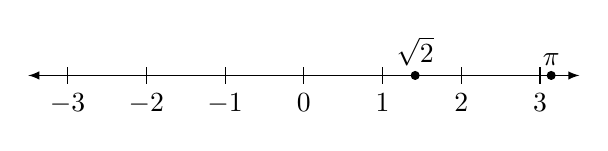
\begin{tikzpicture}
    \draw[latex-latex] (-3.5,0) -- (3.5,0); % The real line
    \foreach \x in {-3, -2, -1, 0, 1, 2, 3} % Points on the line
        \draw[shift={(\x,0)},color=black] (0pt,3pt) -- (0pt,-3pt);
    \foreach \x in {-3, -2, -1, 0, 1, 2, 3} 
        \draw[shift={(\x,0)},color=black] (0pt,0pt) -- (0pt,-3pt) node[below] {$\x$};
    \draw[fill=black] ({sqrt(2)},0) circle (0.05) node[above] {$\sqrt{2}$};
    \draw[fill=black] (pi,0) circle (0.05) node[above] {$\pi$};
\end{tikzpicture}
\end{center}


\subsubsection{Visualizing Rational and Irrational Numbers}
Rational numbers can be precisely located on the real line, whereas irrational numbers cannot be exactly pinpointed due to their non-repeating, non-terminating nature.


\begin{exercise}
Mark the point \( \frac{3}{2} \) on the real line.
\end{exercise}


\begin{exercise}
Explain why it is impossible to accurately mark \( \sqrt{3} \) on the real line.
\end{exercise}


\begin{solution}
Since \( \sqrt{3} \) is an irrational number with a non-repeating, non-terminating decimal, it cannot be accurately represented by a specific point on the real line.
\end{solution}


\subsection*{Practice Problems on Real Numbers and The Real Line}
\addcontentsline{toc}{subsection}{Practice Problems on Real Numbers and The Real Line}


\begin{problem}
Represent the following sets of numbers on the real line:
\begin{enumerate}[label=(\alph*)]
    \item \( \{ x \in \mathbb{R} | x > -2 \} \)
    \item \( \{ x \in \mathbb{R} | -1 \leq x \leq 1 \} \)
    \item \( \{ x \in \mathbb{R} | x < \sqrt{2} \} \)
\end{enumerate}
\end{problem}


\begin{problem}
Identify whether the following numbers are rational or irrational, and justify your answer:
\begin{enumerate}[label=(\alph*)]
    \item \( \frac{5}{7} \)
    \item \( \pi \)
    \item \( 0.3333\ldots \) (repeating)
    \item \( \sqrt{9} \)
\end{enumerate}
\end{problem}


\begin{problem}
On a real line, mark the points corresponding to the following numbers:
\begin{enumerate}[label=(\alph*)]
    \item \( 0 \)
    \item \( -3 \)
    \item \( 2.5 \)
    \item \( -\sqrt{2} \) (approximate the position)
\end{enumerate}
\end{problem}


\begin{problem}
If the distance between the points representing \( x \) and 4 on the real line is 3 units, what could be the possible values of \( x \)?
\end{problem}


\begin{problem}
Explain why the square root of any prime number is an irrational number.
\end{problem}


\begin{exercise}
Graphically represent the interval \( (-\infty, -1] \) on the real line.
\end{exercise}


\begin{exercise}
Determine whether the number \( \frac{22}{7} \) is a rational or irrational number and explain your reasoning.
\end{exercise}


% End of Practice Problems Section


\subsection{Arithmetic Operations}
\label{subsec:arithmetic_operations}
Arithmetic operations form the basis of algebra. They include addition, subtraction, multiplication, and division. Each operation has unique properties that are crucial for simplifying and solving algebraic expressions.


\subsubsection{Addition}
Addition combines two or more numbers into a single sum. Properties of addition include:
\begin{itemize}
    \item \textbf{Commutative Property:} The order of numbers does not change the sum. For any two numbers \( a \) and \( b \), \( a + b = b + a \).
    \item \textbf{Associative Property:} The grouping of numbers does not change the sum. For any three numbers \( a \), \( b \), and \( c \), \( (a + b) + c = a + (b + c) \).
    \item \textbf{Identity Property:} Adding zero to any number does not change the number. For any number \( a \), \( a + 0 = a \).
\end{itemize}


\subsubsection{Subtraction}
Subtraction is the operation of finding the difference between two numbers. It is the inverse of addition. For any two numbers \( a \) and \( b \), \( a - b \) gives the difference.


\subsubsection{Multiplication}
Multiplication is the operation of adding a number to itself a certain number of times. Its properties are:
\begin{itemize}
    \item \textbf{Commutative Property:} The order of numbers does not change the product. For any two numbers \( a \) and \( b \), \( ab = ba \).
    \item \textbf{Associative Property:} The grouping of numbers does not change the product. For any three numbers \( a \), \( b \), and \( c \), \( (ab)c = a(bc) \).
    \item \textbf{Identity Property:} Multiplying any number by one does not change the number. For any number \( a \), \( a \cdot 1 = a \).
    \item \textbf{Distributive Property:} Distributes multiplication over addition. For any numbers \( a \), \( b \), and \( c \), \( a(b + c) = ab + ac \).
\end{itemize}


\subsubsection{Division}
Division is the operation of distributing a number into equal parts. It is the inverse of multiplication. For any two numbers \( a \) and \( b \) (where \( b \neq 0 \)), \( \frac{a}{b} \) gives the quotient.


% Examples and Exercises
\begin{exercise}
Show that \( 3 + 5 = 5 + 3 \) to demonstrate the commutative property of addition.
\end{exercise}


\begin{exercise}
Verify \( 2(3 + 4) = 2 \cdot 3 + 2 \cdot 4 \) using the distributive property of multiplication.
\end{exercise}


\begin{problem}
If \( x = 7 \) and \( y = 3 \), calculate and compare \( x + y \) and \( y + x \).
\end{problem}


\begin{problem}
Simplify the expression \( 4 \times (x + 5) \) using the distributive property.
\end{problem}


% End of Arithmetic Operations Section


\subsection*{Practice Problems on Arithmetic Operations}
\addcontentsline{toc}{subsection}{Practice Problems on Arithmetic Operations}


\begin{problem}
Solve the following arithmetic expressions:
\begin{enumerate}[label=(\alph*)]
    \item \( 9 + 6 \)
    \item \( 20 - 7 \)
    \item \( 4 \times 5 \)
    \item \( 18 \div 2 \)
\end{enumerate}
\end{problem}


\begin{problem}
Using the associative property of addition, show that \( (2 + 3) + 4 = 2 + (3 + 4) \).
\end{problem}


\begin{problem}
Apply the distributive property to simplify and calculate \( 3(5 + 2) \).
\end{problem}


\begin{problem}
If \( a = 10 \) and \( b = 5 \), calculate the following expressions:
\begin{enumerate}[label=(\alph*)]
    \item \( a + b \)
    \item \( a - b \)
    \item \( a \times b \)
    \item \( a \div b \), ensuring \( b \neq 0 \)
\end{enumerate}
\end{problem}


\begin{problem}
Demonstrate the commutative property of multiplication with \( a = 6 \) and \( b = 3 \) by showing that \( ab = ba \).
\end{problem}


\begin{exercise}
For the given values \( x = 3 \) and \( y = 2 \), calculate \( 2x + 3y \).
\end{exercise}


\begin{exercise}
Show the identity property of multiplication by verifying that \( 9 \times 1 = 9 \).
\end{exercise}


% End of Practice Problems Section


\subsection{Exponents and Radicals}
\label{subsec:exponents_and_radicals}
Exponents and radicals are fundamental algebra operations with specific rules and properties. Understanding these rules is crucial for simplifying and solving algebraic expressions.


\subsubsection{Rules of Exponents}
The rules of exponents apply to expressions where numbers are raised to a power. The key rules include:
\begin{itemize}
    \item \textbf{Product Rule:} \( a^n \times a^m = a^{n+m} \)
    \item \textbf{Quotient Rule:} \( \frac{a^n}{a^m} = a^{n-m} \), where \( a \neq 0 \)
    \item \textbf{Power Rule:} \( (a^n)^m = a^{nm} \)
    \item \textbf{Zero Exponent Rule:} \( a^0 = 1 \), where \( a \neq 0 \)
    \item \textbf{Negative Exponent Rule:} \( a^{-n} = \frac{1}{a^n} \), where \( a \neq 0 \)
\end{itemize}


\subsubsection{Radicals}
Radicals involve finding roots of numbers. The most common radical is the square root, but higher roots (such as cube roots) are also used.


\begin{itemize}
    \item \textbf{Simplifying Radicals:} \( \sqrt{a^2} = a \) for any positive real number \( a \).
    \item \textbf{Multiplication and Division:} \( \sqrt{a} \times \sqrt{b} = \sqrt{ab} \) and \( \frac{\sqrt{a}}{\sqrt{b}} = \sqrt{\frac{a}{b}} \), where \( a \) and \( b \) are positive.
\end{itemize}


% Examples and Exercises
\begin{exercise}
Simplify \( 2^3 \times 2^4 \) using the product rule of exponents.
\end{exercise}


\begin{exercise}
Calculate \( \sqrt{9} \times \sqrt{16} \) and compare it to \( \sqrt{9 \times 16} \).
\end{exercise}


\begin{problem}
If \( x = 2 \), simplify and calculate \( x^{-3} \) using the negative exponent rule.
\end{problem}


\begin{problem}
Express \( \frac{1}{x^2} \) as an exponent with a negative power.
\end{problem}


% End of Exponents and Radicals Section


\subsection*{Practice Problems on Exponents and Radicals}
\addcontentsline{toc}{subsection}{Practice Problems on Exponents and Radicals}


\begin{problem}
Simplify the following expressions involving exponents:
\begin{enumerate}[label=(\alph*)]
    \item \( 5^3 \times 5^2 \)
    \item \( \frac{4^5}{4^2} \)
    \item \( (3^2)^3 \)
    \item \( 6^0 \)
    \item \( 2^{-4} \)
\end{enumerate}
\end{problem}


\begin{problem}
Calculate and simplify the following radical expressions:
\begin{enumerate}[label=(\alph*)]
    \item \( \sqrt{25} \)
    \item \( \sqrt{8} \times \sqrt{2} \)
    \item \( \frac{\sqrt{49}}{\sqrt{7}} \)
    \item \( \sqrt[3]{27} \)
\end{enumerate}
\end{problem}


\begin{problem}
Express the following expressions with positive exponents:
\begin{enumerate}[label=(\alph*)]
    \item \( x^{-2} \)
    \item \( \frac{1}{y^{-3}} \)
\end{enumerate}
\end{problem}


\begin{problem}
If \( a = 4 \), find the value of \( a^{-1/2} \).
\end{problem}


\begin{exercise}
For the given value \( x = 2 \), calculate and simplify \( x^3 \times x^2 \).
\end{exercise}


\begin{exercise}
Simplify the expression \( \sqrt{9} + \sqrt{16} \).
\end{exercise}


% End of Practice Problems Section


\section{Equations and Inequalities}
\label{sec:equations_and_inequalities}
Understanding how to manipulate and solve equations and inequalities is vital in calculus.


\subsection{Linear Equations}
\label{subsec:linear_equations}
This section covers the techniques for solving linear equations. Various examples and practice problems will be included to demonstrate these methods and provide students with hands-on experience in solving different types of linear equations.


\subsubsection{Single Variable Linear Equations}
This section discusses the methods for solving linear equations with one variable. A linear equation in one variable can be written in the form \( ax + b = 0 \), where \( a \) and \( b \) are constants, and \( x \) is the variable to be solved for.

\paragraph{Balancing Equations}
The principle of balancing equations involves performing the same operation on both sides of the equation to maintain equality. Common operations include addition, subtraction, multiplication, and division.

\paragraph{Isolating the Variable}
To find the value of the variable, the goal is to isolate it on one side of the equation. This is typically achieved by:
\begin{itemize}
    \item Adding or subtracting the same number from both sides of the equation.
    \item Multiplying or dividing both sides of the equation by the same number (except zero).
\end{itemize}

% Example Problems
\begin{problem}
Solve the equation \( 3x + 6 = 12 \).
\end{problem}

\begin{solution}
Subtract 6 from both sides: \( 3x = 6 \).\\
Divide both sides by 3: \( x = 2 \).
\end{solution}

\begin{problem}
Solve \( 2(x - 3) = 4 \).
\end{problem}

\begin{solution}
Expand and simplify: \( 2x - 6 = 4 \).\\
Add 6 to both sides: \( 2x = 10 \).\\
Divide both sides by 2: \( x = 5 \).
\end{solution}

% Exercises
\begin{exercise}
Solve the equation \( 5x - 15 = 0 \).
\end{exercise}

\begin{exercise}
Find the value of \( x \) in the equation \( 7 - 2x = -9 \).
\end{exercise}

% End of Single Variable Linear Equations Section

\subsection*{Practice Problems on Single Variable Linear Equations}
\addcontentsline{toc}{subsection}{Practice Problems on Single Variable Linear Equations}

\begin{problem}
Solve the following linear equations:
\begin{enumerate}[label=(\alph*)]
    \item \( 4x + 8 = 20 \)
    \item \( 3x - 9 = 0 \)
    \item \( x + 5 = 2 \)
    \item \( 6 - 2x = 0 \)
    \item \( 7x = 49 \)
\end{enumerate}
\end{problem}

\begin{problem}
For each equation, first expand and then solve for \( x \):
\begin{enumerate}[label=(\alph*)]
    \item \( 2(3x - 4) = 14 \)
    \item \( 5(x + 2) - 3 = 22 \)
    \item \( 4 - 2(2x - 3) = 8 \)
\end{enumerate}
\end{problem}

\begin{problem}
Find the value of \( x \) in the following equations:
\begin{enumerate}[label=(\alph*)]
    \item \( 10x + 5 = 3x + 20 \)
    \item \( 5x - 2 = 2x + 7 \)
    \item \( \frac{x}{2} + 3 = 7 \)
    \item \( 3x - \frac{x}{4} = 8 \)
\end{enumerate}
\end{problem}

\begin{exercise}
If \( 4x + 6 = 2x + 14 \), what is the value of \( x \)?
\end{exercise}

\begin{exercise}
Solve the equation \( \frac{5x - 3}{2} = 6 \).
\end{exercise}

% End of Practice Problems Section

\subsubsection{Systems of Linear Equations}
Solving systems of linear equations is a key skill in algebra. There are primarily two methods for solving these systems:

\paragraph{Substitution Method}
This method involves solving one of the equations for one variable and then substituting that expression into the other equation. It is particularly useful when one of the equations is already solved for one variable.

% Example using substitution method
\begin{problem}
Solve the system using the substitution method:
\begin{align*}
    x + y &= 10 \\
    y &= 3x
\end{align*}
\end{problem}

\begin{solution}
Substitute \( y \) from the second equation into the first equation:\\
\( x + 3x = 10 \)\\
\( 4x = 10 \)\\
\( x = \frac{10}{4} = 2.5 \)\\
Now substitute \( x \) back into the second equation to find \( y \):\\
\( y = 3(2.5) = 7.5 \)
\end{solution}

\paragraph{Elimination Method}
This method involves adding or subtracting the equations to eliminate one of the variables. It is useful when the coefficients of one of the variables are the same or opposites.

% Example using elimination method
\begin{problem}
Solve the system using the elimination method:
\begin{align*}
    2x + 3y &= 8 \\
    4x - 3y &= 12
\end{align*}
\end{problem}

\begin{solution}
Add the two equations to eliminate \( y \):\\
\( (2x + 3y) + (4x - 3y) = 8 + 12 \)\\
\( 6x = 20 \)\\
\( x = \frac{20}{6} \approx 3.33 \)\\
Now substitute \( x \) into one of the equations to find \( y \).
\end{solution}

% Exercises
\begin{exercise}
Use the substitution method to solve:
\begin{align*}
    x - y &= 2 \\
    2x + y &= 7
\end{align*}
\end{exercise}

\begin{exercise}
Use the elimination method to solve:
\begin{align*}
    3x + y &= 6 \\
    x - 2y &= 3
\end{align*}
\end{exercise}

% End of Systems of Linear Equations Section

\subsection*{Practice Problems on Systems of Linear Equations}
\addcontentsline{toc}{subsection}{Practice Problems on Systems of Linear Equations}

\begin{problem}
Use the substitution method to solve the following systems of equations:
\begin{enumerate}[label=(\alph*)]
    \item 
    \begin{align*}
        x + 2y &= 5 \\
        y &= 2x - 1
    \end{align*}
    \item 
    \begin{align*}
        3x - y &= 7 \\
        x + y &= 9
    \end{align*}
\end{enumerate}
\end{problem}

\begin{problem}
Solve the following systems using the elimination method:
\begin{enumerate}[label=(\alph*)]
    \item 
    \begin{align*}
        x + y &= 4 \\
        2x - y &= 1
    \end{align*}
    \item 
    \begin{align*}
        4x + 5y &= 20 \\
        -3x + 2y &= -6
    \end{align*}
\end{enumerate}
\end{problem}

\begin{problem}
Determine the solution for each system of equations:
\begin{enumerate}[label=(\alph*)]
    \item 
    \begin{align*}
        2x + 3y &= 6 \\
        x - 2y &= 3
    \end{align*}
    \item 
    \begin{align*}
        y &= x + 1 \\
        2x + 3y &= 12
    \end{align*}
\end{enumerate}
\end{problem}

\begin{exercise}
Find the values of \( x \) and \( y \) for:
\begin{align*}
    x - y &= 3 \\
    3x + 2y &= 12
\end{align*}
\end{exercise}

\begin{exercise}
Solve the following system using any method:
\begin{align*}
    x + 2y &= 7 \\
    2x - y &= 4
\end{align*}
\end{exercise}

% End of Practice Problems Section

\subsection{Polynomial Equations}
\label{subsec:polynomial_equations}
Polynomial equations are algebraic expressions that involve variables raised to whole number exponents. Understanding how to solve these equations is a fundamental skill in algebra.

\subsubsection{Characteristics of Polynomial Equations}
A polynomial equation can be written in the form:
\[ a_nx^n + a_{n-1}x^{n-1} + \ldots + a_1x + a_0 = 0 \]
where \( a_n, a_{n-1}, \ldots, a_1, a_0 \) are constants, and \( n \) is a non-negative integer.

\subsubsection{Solving Polynomial Equations}
Methods for solving polynomial equations include:

\paragraph{Factoring:} Expressing the polynomial as a product of its factors.
\paragraph{Using the Quadratic Formula:} Applicable to quadratic equations of the form \( ax^2 + bx + c = 0 \).
\paragraph{Graphical Methods:} Plotting the polynomial to find the points where it intersects the x-axis.

\subsubsection{Fundamental Theorem of Algebra}
The Fundamental Theorem of Algebra states that every non-constant polynomial equation has at least one complex root. This implies that a polynomial of degree \( n \) will have \( n \) roots (counting multiplicity).

% Examples and Exercises
\begin{problem}
Solve the quadratic equation \( x^2 - 5x + 6 = 0 \) by factoring.
\end{problem}

\begin{solution}
Factorize the equation: \( (x - 2)(x - 3) = 0 \).\\
Thus, the solutions are \( x = 2 \) and \( x = 3 \).
\end{solution}

\begin{problem}
Use the quadratic formula to solve \( 2x^2 - 4x - 6 = 0 \).
\end{problem}

\begin{solution}
Apply the quadratic formula: \( x = \frac{-b \pm \sqrt{b^2 - 4ac}}{2a} \).\\
Here, \( a = 2 \), \( b = -4 \), and \( c = -6 \).\\
Calculate the roots using these values.
\end{solution}

\begin{exercise}
Factorize and solve the polynomial \( x^3 - 7x^2 + 14x - 8 = 0 \).
\end{exercise}

\begin{exercise}
Plot the graph of \( y = x^2 - 4x + 3 \) and find the roots.
\end{exercise}

% End of Polynomial Equations Section

\subsection*{Practice Problems on Polynomial Equations}
\addcontentsline{toc}{subsection}{Practice Problems on Polynomial Equations}

\begin{problem}
Factorize and solve the following polynomial equations:
\begin{enumerate}[label=(\alph*)]
    \item \( x^2 - 9 = 0 \)
    \item \( x^2 - 6x + 8 = 0 \)
    \item \( x^3 - x^2 - 4x + 4 = 0 \)
\end{enumerate}
\end{problem}

\begin{problem}
Use the quadratic formula to find the roots of the following equations:
\begin{enumerate}[label=(\alph*)]
    \item \( 3x^2 - 2x - 5 = 0 \)
    \item \( x^2 + 4x + 4 = 0 \)
\end{enumerate}
\end{problem}

\begin{problem}
Given the polynomial \( x^3 - 3x^2 + 4 \), determine:
\begin{enumerate}[label=(\alph*)]
    \item The degree of the polynomial.
    \item The leading coefficient.
    \item The constant term.
\end{enumerate}
\end{problem}

\begin{exercise}
For the polynomial equation \( 2x^2 - 8x = 0 \), find the values of \( x \).
\end{exercise}

\begin{exercise}
Solve \( x^3 + 2x^2 - 5x - 6 = 0 \) by factoring.
\end{exercise}

% End of Practice Problems Section

\subsection{Rational Equations and Inequalities}
\label{subsec:rational_equations_inequalities}
Rational equations and inequalities involve expressions where variables appear in the denominator. Solving these requires careful manipulation to avoid undefined expressions (like division by zero).

\subsubsection{Solving Rational Equations}
Solving rational equations typically involves finding a common denominator, clearing the fractions, and then solving the resulting equation. Steps include:

\begin{enumerate}
    \item Identify the least common denominator (LCD) of all fractions in the equation.
    \item Multiply each term of the equation by the LCD to eliminate the fractions.
    \item Solve the resulting equation using appropriate algebraic methods.
\end{enumerate}

\subsubsection{Solving Rational Inequalities}
Solving rational inequalities involves finding the values of the variable for which the inequality holds true. Steps include:

\begin{enumerate}
    \item Rewrite the inequality as an equation and find the critical points (where the rational expression is zero or undefined).
    \item Determine the intervals of the variable by testing points around the critical points.
    \item Conclude the solution set based on the tests.
\end{enumerate}

% Example Problems and Exercises
\begin{problem}
Solve the rational equation \( \frac{1}{x} + \frac{1}{x-2} = \frac{1}{x-1} \).
\end{problem}

\begin{solution}
Find the LCD, clear fractions, and solve the resulting equation.
\end{solution}

\begin{problem}
Solve the inequality \( \frac{x-3}{x+2} \leq 0 \).
\end{problem}

\begin{solution}
Find the critical points and test intervals to determine where the inequality holds true.
\end{solution}

\begin{exercise}
Solve \( \frac{2}{x} - \frac{3}{x+1} = \frac{1}{x-1} \).
\end{exercise}

\begin{exercise}
Determine the solution set for \( \frac{x+1}{x-2} > 1 \).
\end{exercise}

% End of Rational Equations and Inequalities Section

\subsection*{Practice Problems on Rational Equations and Inequalities}
\addcontentsline{toc}{subsection}{Practice Problems on Rational Equations and Inequalities}

\begin{problem}
Solve the following rational equations:
\begin{enumerate}[label=(\alph*)]
    \item \( \frac{2}{x} + \frac{3}{x+4} = \frac{5}{x-1} \)
    \item \( \frac{1}{x+2} - \frac{1}{x} = \frac{1}{2} \)
\end{enumerate}
\end{problem}

\begin{problem}
Solve the following rational inequalities:
\begin{enumerate}[label=(\alph*)]
    \item \( \frac{x+1}{x-3} \geq 0 \)
    \item \( \frac{2x}{x-2} < 3 \)
\end{enumerate}
\end{problem}

\begin{problem}
Find the value of \( x \) for which the rational expression \( \frac{x^2 - 4}{x^2 - 5x + 6} \) is undefined.
\end{problem}

\begin{exercise}
Solve the equation \( \frac{1}{x+3} + \frac{1}{2x} = \frac{3}{4} \).
\end{exercise}

\begin{exercise}
Determine the solution set for the inequality \( \frac{x+2}{x-1} \leq 2 \).
\end{exercise}

% End of Practice Problems Section

\subsection{Inequalities}
\label{subsec:inequalities}
Inequalities are mathematical expressions involving the symbols \( > \), \( < \), \( \geq \), or \( \leq \). They show the relationship between two values. Solving inequalities often involves finding the set of values that make the inequality true.

\subsubsection{Solving Linear Inequalities}
Linear inequalities are similar to linear equations but with inequality symbols. The steps to solve them are:
\begin{enumerate}
    \item Isolate the variable on one side of the inequality.
    \item Perform the same operation on both sides of the inequality.
    \item If you multiply or divide by a negative number, reverse the inequality sign.
\end{enumerate}

\subsubsection{Solving Quadratic Inequalities}
Quadratic inequalities involve a quadratic expression. To solve them:
\begin{enumerate}
    \item Bring all terms to one side of the inequality to form a quadratic equation.
    \item Solve the corresponding quadratic equation.
    \item Determine the intervals where the inequality holds by testing values or using a sign chart.
\end{enumerate}

% Example Problems
\begin{problem}
Solve the inequality \( 3x - 4 > 2 \).
\end{problem}

\begin{solution}
Add 4 to both sides: \( 3x > 6 \).\\
Divide by 3: \( x > 2 \).
\end{solution}

\begin{problem}
Solve the quadratic inequality \( x^2 - 5x + 6 \leq 0 \).
\end{problem}

\begin{solution}
Factorize the quadratic: \( (x - 2)(x - 3) \leq 0 \).\\
Determine the intervals and test points.
\end{solution}

% Graphical Representation using TikZ
\begin{center}
\begin{tikzpicture}
\begin{axis}[
    axis lines=middle,
    xlabel=\(x\),
    ylabel=\(y\),
    xmin=-1, xmax=4,
    ymin=-1, ymax=2,
    xtick={2,3},
    ytick=\empty,
    clip=false
]
\addplot[name path=f,blue,domain=-1:4] {x^2 - 5*x + 6};
\path[name path=axis] (axis cs:-1,0) -- (axis cs:4,0);
\addplot[blue!50] fill between[of=f and axis,soft clip={domain=2:3}];
\node[blue,right] at (axis cs: 1,2) {\(x^2 - 5x + 6 \leq 0\)};
\end{axis}
\end{tikzpicture}
\end{center}

% Exercises
\begin{exercise}
Solve the inequality \( 2x + 3 \leq 7 \).
\end{exercise}

\begin{exercise}
Determine the solution set for \( x^2 - x - 6 > 0 \).
\end{exercise}

% End of Inequalities Section

\subsection*{Practice Problems on Inequalities}
\addcontentsline{toc}{subsection}{Practice Problems on Inequalities}

\begin{problem}
Solve the following linear inequalities:
\begin{enumerate}[label=(\alph*)]
    \item \( 5x - 7 > 3 \)
    \item \( 2 - 3x \leq 8 \)
    \item \( 4(2x + 1) \geq 3x - 2 \)
\end{enumerate}
\end{problem}

\begin{problem}
Determine the solution set for the following quadratic inequalities:
\begin{enumerate}[label=(\alph*)]
    \item \( x^2 - 4x + 3 < 0 \)
    \item \( x^2 + x - 6 \geq 0 \)
    \item \( -x^2 + 6x - 5 > 0 \)
\end{enumerate}
\end{problem}

\begin{problem}
For each inequality, graph the solution set on a number line:
\begin{enumerate}[label=(\alph*)]
    \item \( x + 5 > 0 \)
    \item \( x^2 - x - 2 \leq 0 \)
\end{enumerate}
\end{problem}

\begin{exercise}
Solve and graph the solution set for \( 3x + 4 < 2x - 1 \).
\end{exercise}

\begin{exercise}
Find the values of \( x \) for which \( x^2 - 5x + 6 \leq 0 \) and represent the solution graphically.
\end{exercise}

% End of Practice Problems Section

\subsection{Quadratic Equations}
\label{subsec:quadratic_equations}
Quadratic equations are polynomial equations of the second degree, typically in the form \( ax^2 + bx + c = 0 \), where \( a \), \( b \), and \( c \) are constants, and \( a \neq 0 \). There are several methods to solve these equations.

\subsubsection{Factoring}
Factoring involves expressing the quadratic equation as a product of its factors, if possible. The solutions are the values of \( x \) for which each factor equals zero.

\subsubsection{Completing the Square}
This method involves rearranging the equation and completing the square to solve for \( x \). It is particularly useful when the quadratic equation cannot be factored easily.

\subsubsection{Quadratic Formula}
The quadratic formula is a universal method that can solve any quadratic equation. It is given by:
\[ x = \frac{-b \pm \sqrt{b^2 - 4ac}}{2a} \]

% Example Problems
\begin{problem}
Solve the quadratic equation \( x^2 - 5x + 6 = 0 \) by factoring.
\end{problem}

\begin{problem}
Use completing the square to solve \( x^2 + 4x - 5 = 0 \).
\end{problem}

\begin{problem}
Apply the quadratic formula to solve \( 2x^2 - 3x + 1 = 0 \).
\end{problem}

% Graphical Representation using TikZ
\begin{center}
\begin{tikzpicture}
\begin{axis}[
    axis lines=middle,
    xlabel=\(x\),
    ylabel=\(y\),
    domain=-3:3,
    xmin=-3, xmax=3,
    ymin=-10, ymax=10,
    samples=200,
    xtick={-3,-2,...,3},
    ytick={-10,-8,...,10},
    clip=false
]
\addplot[blue,thick] {x^2 - 5*x + 6};
\node[blue,right] at (axis cs: 1, 4) {\(y = x^2 - 5x + 6\)};
\end{axis}
\end{tikzpicture}
\end{center}

% Exercises
\begin{exercise}
Factorize and solve \( x^2 - x - 6 = 0 \).
\end{exercise}

\begin{exercise}
Use the quadratic formula to find the roots of \( 3x^2 + 2x - 1 = 0 \).
\end{exercise}

% End of Quadratic Equations Section

\subsection*{Practice Problems on Quadratic Equations}
\addcontentsline{toc}{subsection}{Practice Problems on Quadratic Equations}

\begin{problem}
Solve the following quadratic equations by factoring:
\begin{enumerate}[label=(\alph*)]
    \item \( x^2 - 7x + 10 = 0 \)
    \item \( x^2 + 9x + 18 = 0 \)
\end{enumerate}
\end{problem}

\begin{problem}
Use the method of completing the square to solve these equations:
\begin{enumerate}[label=(\alph*)]
    \item \( x^2 + 6x + 8 = 0 \)
    \item \( x^2 - 4x - 5 = 0 \)
\end{enumerate}
\end{problem}

\begin{problem}
Apply the quadratic formula to solve:
\begin{enumerate}[label=(\alph*)]
    \item \( 2x^2 - 4x - 6 = 0 \)
    \item \( 3x^2 + x - 2 = 0 \)
\end{enumerate}
\end{problem}

\begin{exercise}
Factorize and solve \( x^2 - 2x - 15 = 0 \).
\end{exercise}

\begin{exercise}
Find the roots of the quadratic equation \( x^2 + 12x + 35 = 0 \) using the quadratic formula.
\end{exercise}

% End of Practice Problems Section

\subsection{Inequalities and Absolute Values}
\label{subsec:inequalities_absolute_values}
Inequalities and absolute values are fundamental concepts in algebra. This section explores how to solve these types of problems.

\subsubsection{Solving Linear Inequalities}
Linear inequalities are solved similarly to linear equations, but the solution is typically a range of values rather than a single number. Key steps include isolating the variable and remembering to reverse the inequality sign when multiplying or dividing by a negative number.

\subsubsection{Solving Quadratic Inequalities}
Quadratic inequalities can be solved by finding the roots of the corresponding quadratic equation and then testing intervals to determine where the inequality holds true.

\subsubsection{Absolute Value}
The absolute value of a number is its distance from zero on the number line, regardless of direction. Solving equations with absolute values often involves considering two separate cases, based on the definition of absolute value.

% Example Problems
\begin{problem}
Solve the inequality \( 2x - 3 < 5 \).
\end{problem}

\begin{problem}
Determine the solution set for the quadratic inequality \( x^2 - 4x + 3 > 0 \).
\end{problem}

\begin{problem}
Solve the absolute value equation \( |x + 2| = 5 \).
\end{problem}

% Graphical Representation using TikZ for Absolute Value
\begin{center}
\begin{tikzpicture}
\begin{axis}[
    axis lines=middle,
    xlabel=\(x\),
    ylabel=\(y\),
    xmin=-10, xmax=10,
    ymin=-10, ymax=10,
    clip=false
]
\addplot[blue, domain=-10:10, samples=100] {abs(x + 2)};
\node[blue, right] at (axis cs: 3, 5) {\(|x + 2|\)};
\draw[dashed] (axis cs:-7,5) -- (axis cs:3,5);
\end{axis}
\end{tikzpicture}
\end{center}

% Exercises
\begin{exercise}
Solve the inequality \( -3 \leq 4x + 1 < 11 \).
\end{exercise}

\begin{exercise}
Find the values of \( x \) for which \( |3x - 4| \leq 2 \).
\end{exercise}

% End of Inequalities and Absolute Values Section

\subsection*{Practice Problems on Inequalities and Absolute Values}
\addcontentsline{toc}{subsection}{Practice Problems on Inequalities and Absolute Values}

\begin{problem}
Solve the following linear inequalities:
\begin{enumerate}[label=(\alph*)]
    \item \( 5x + 7 > 12 \)
    \item \( 3 - 2x \leq 1 \)
    \item \( -4x + 5 \geq 9 \)
\end{enumerate}
\end{problem}

\begin{problem}
Determine the solution sets for these quadratic inequalities:
\begin{enumerate}[label=(\alph*)]
    \item \( x^2 - x - 6 < 0 \)
    \item \( 2x^2 + 3x - 2 > 0 \)
\end{enumerate}
\end{problem}

\begin{problem}
Solve the following absolute value equations and inequalities:
\begin{enumerate}[label=(\alph*)]
    \item \( |x - 3| = 8 \)
    \item \( |2x + 4| \leq 6 \)
    \item \( |x^2 - 4| > 3 \)
\end{enumerate}
\end{problem}

\begin{exercise}
Solve the inequality \( -2 \leq x - 5 < 4 \).
\end{exercise}

\begin{exercise}
Find the values of \( x \) that satisfy \( |x + 1| > 5 \).
\end{exercise}

% End of Practice Problems Section


\section{Functions and Their Properties}
\label{sec:functions_and_properties}
A deep understanding of functions and their characteristics is essential in calculus.

\subsection{Concept of a Function}
\label{subsec:concept_of_function}
A function is a relation between a set of inputs and a set of permissible outputs, where each input is related to exactly one output. 

\subsubsection{Types of Functions}
\begin{itemize}
    \item \textbf{Linear Function:} A function of the form \( f(x) = mx + b \), where \( m \) and \( b \) are constants.
    \item \textbf{Quadratic Function:} A function represented by \( f(x) = ax^2 + bx + c \), where \( a \), \( b \), and \( c \) are constants.
    \item \textbf{Polynomial Function:} A function that is the sum of multiple terms, each of which is a product of a constant and a variable raised to a non-negative integer power.
\end{itemize}

\subsubsection{Domain and Range}
\begin{itemize}
    \item \textbf{Domain:} The set of all possible input values for the function.
    \item \textbf{Range:} The set of all possible output values.
\end{itemize}

\subsubsection{Function vs. Relation}
While a relation can relate an input to multiple outputs, a function assigns each input exactly one output.

\subsubsection{Set Notation}
In discussing functions, set notation is often used to describe the domain and range. For example, if the domain of \( f(x) \) is all real numbers, it is denoted as \( \text{dom}(f) = \mathbb{R} \).

% Graphical Representations
\begin{center}
\begin{tikzpicture}
\begin{axis}[
    axis lines=middle,
    xlabel=\(x\),
    ylabel={\(f(x)\)},
    xmin=-5, xmax=5,
    ymin=-5, ymax=5,
    xtick={-4,-3,...,4},
    ytick={-4,-3,...,4},
    clip=false
]
\addplot[blue, domain=-5:5, samples=100] {x^2 - 4};
\node[blue, right] at (axis cs: 2, 2) {\(f(x) = x^2 - 4\)};
\end{axis}
\end{tikzpicture}
\end{center}

% Exercises
\begin{exercise}
What is the domain and range of the function \( g(x) = \sqrt{x} \)?
\end{exercise}

\begin{exercise}
Is the relation \( R = \{(1, 2), (1, 3), (2, 3)\} \) a function? Explain your reasoning.
\end{exercise}

% End of Concept of a Function Section

\subsection*{Practice Problems on the Concept of a Function}
\addcontentsline{toc}{subsection}{Practice Problems on the Concept of a Function}

\begin{problem}
Determine the domain and range of the following functions:
\begin{enumerate}[label=(\alph*)]
    \item \( f(x) = 2x + 3 \)
    \item \( g(x) = x^2 - 4 \)
    \item \( h(x) = \frac{1}{x - 2} \)
\end{enumerate}
\end{problem}

\begin{problem}
Identify whether each of the following relations is a function. Provide reasons for your answer:
\begin{enumerate}[label=(\alph*)]
    \item \( \{(1, 2), (2, 3), (3, 4)\} \)
    \item \( \{(2, 3), (2, 4), (3, 5)\} \)
    \item \( \{(x, y) | y = x^2\} \)
\end{enumerate}
\end{problem}

\begin{problem}
For each function, describe its type (linear, quadratic, etc.) and sketch its graph:
\begin{enumerate}[label=(\alph*)]
    \item \( f(x) = -3x \)
    \item \( g(x) = x^2 + 2x + 1 \)
\end{enumerate}
\end{problem}

\begin{exercise}
Find the domain and range of the function \( f(x) = \sqrt{x + 4} \).
\end{exercise}

\begin{exercise}
Is the set \( \{(x, y) | x^2 + y^2 = 25\} \) a function? Justify your answer.
\end{exercise}

% End of Practice Problems Section

\subsection{Function Notation and Graphs}
\label{subsec:function_notation_and_graphs}
Function notation is a way to denote functions in a concise manner. It involves the use of the symbol \( f(x) \), where \( f \) represents the function and \( x \) is the variable.

\subsubsection{Graphing Functions}
Graphing a function involves plotting points whose coordinates satisfy the function and connecting these points to form a curve. The x-axis represents the input values, while the y-axis represents the output values.

\subsubsection{Transformations of Functions}
Transformations include shifting, stretching, or reflecting the graph of a function. Common transformations are:

\begin{itemize}
    \item \textbf{Vertical Shifts:} \( f(x) + k \) shifts the function \( k \) units upwards.
    \item \textbf{Horizontal Shifts:} \( f(x - h) \) shifts the function \( h \) units to the right.
    \item \textbf{Vertical Stretch/Compression:} \( af(x) \) stretches or compresses the function vertically.
    \item \textbf{Reflections:} \( -f(x) \) reflects the function across the x-axis.
\end{itemize}

% Graphical Representation using TikZ and pgfplots
\begin{center}
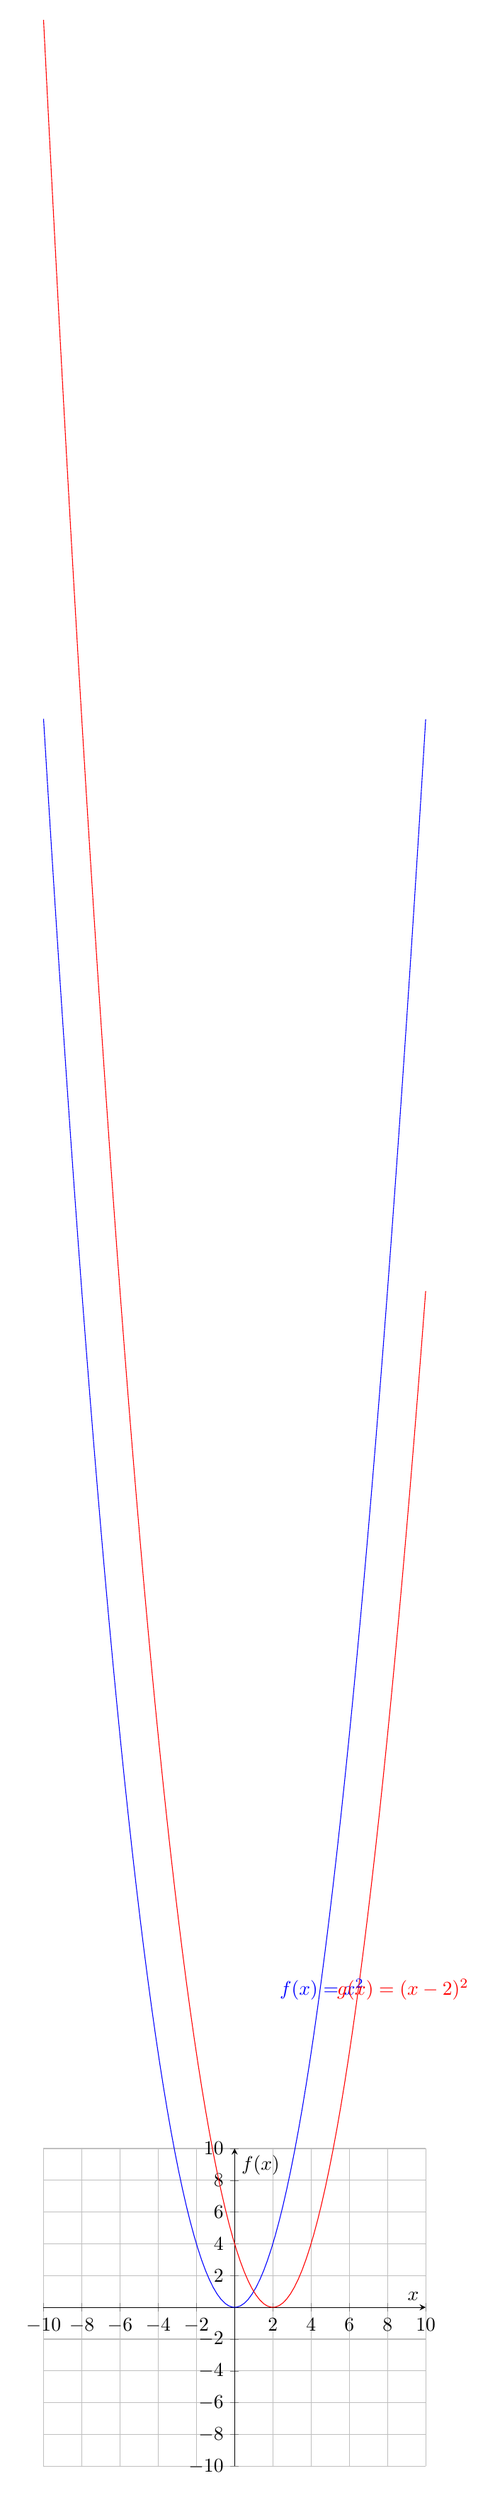
\begin{tikzpicture}
\begin{axis}[
    axis lines = middle,
    xlabel = \(x\),
    ylabel = {\(f(x)\)},
    xmin=-10, xmax=10,
    ymin=-10, ymax=10,
    grid=both,
    xtick={-10,-8,...,10},
    ytick={-10,-8,...,10},
    clip=false
]
\addplot[blue, domain=-10:10, samples=100] {x^2};
\addplot[red, domain=-10:10, samples=100] {(x-2)^2};
\node[blue, right] at (axis cs: 2, 20) {\(f(x) = x^2\)};
\node[red, right] at (axis cs: 5, 20) {\(g(x) = (x - 2)^2\)};
\end{axis}
\end{tikzpicture}
\end{center}

% Exercises
\begin{exercise}
Graph the function \( f(x) = x^2 - 4 \) and describe its transformation compared to \( f(x) = x^2 \).
\end{exercise}

\begin{exercise}
Sketch the graph of \( f(x) = -2(x + 3)^2 + 1 \) and explain the transformations applied to \( f(x) = x^2 \).
\end{exercise}

% End of Function Notation and Graphs Section

\subsection*{Practice Problems on Function Notation and Graphs}
\addcontentsline{toc}{subsection}{Practice Problems on Function Notation and Graphs}

\begin{problem}
Graph the following functions and describe any transformations from the basic function:
\begin{enumerate}[label=(\alph*)]
    \item \( f(x) = (x + 2)^2 \)
    \item \( g(x) = x^2 - 3 \)
    \item \( h(x) = -x^2 + 2 \)
\end{enumerate}
\end{problem}

\begin{problem}
For each function, state its domain and range:
\begin{enumerate}[label=(\alph*)]
    \item \( f(x) = 2x + 1 \)
    \item \( g(x) = \frac{1}{x - 3} \)
    \item \( h(x) = \sqrt{x + 4} \)
\end{enumerate}
\end{problem}

\begin{problem}
Determine the transformations applied to the basic function \( f(x) = x \) for each of the following:
\begin{enumerate}[label=(\alph*)]
    \item \( f(x) = 2x + 3 \)
    \item \( f(x) = -x - 2 \)
    \item \( f(x) = \frac{1}{2}x - 1 \)
\end{enumerate}
\end{problem}

\begin{exercise}
Sketch the graph of \( f(x) = 3x + 2 \) and determine its domain and range.
\end{exercise}

\begin{exercise}
Graph the function \( f(x) = x^2 + 2x - 3 \) and describe the vertex and axis of symmetry.
\end{exercise}

% End of Practice Problems Section

\subsection{Composite and Inverse Functions}
\label{subsec:composite_and_inverse_functions}
The concepts of composite and inverse functions are key in understanding function operations and their applications.

\subsubsection{Composite Functions}
A composite function is the application of one function to the results of another. The notation \( (f \circ g)(x) \) represents the composite function of \( f \) and \( g \), defined as \( f(g(x)) \).

% Example of Composite Function
\begin{example}
If \( f(x) = 2x + 3 \) and \( g(x) = x^2 \), find \( (f \circ g)(x) \) and \( (g \circ f)(x) \).
\end{example}

\subsubsection{Inverse Functions}
An inverse function reverses the operation of a function. The notation \( f^{-1}(x) \) denotes the inverse of function \( f \). A function \( f \) has an inverse if and only if it is one-to-one (bijective).

% Example of Finding an Inverse Function
\begin{example}
Find the inverse of the function \( f(x) = 3x - 2 \).
\end{example}

% Exercises
\begin{exercise}
Given \( f(x) = x + 1 \) and \( g(x) = 2x \), find \( (f \circ g)(x) \) and \( (g \circ f)(x) \).
\end{exercise}

\begin{exercise}
Determine if the function \( f(x) = x^2 \) has an inverse. If it does, find \( f^{-1}(x) \).
\end{exercise}

% End of Composite and Inverse Functions Section

\subsection*{Practice Problems on Composite and Inverse Functions}
\addcontentsline{toc}{subsection}{Practice Problems on Composite and Inverse Functions}

\begin{problem}
Compute the composite functions for the following pairs of functions:
\begin{enumerate}[label=(\alph*)]
    \item \( f(x) = x^2 \) and \( g(x) = x + 1 \). Find \( (f \circ g)(x) \) and \( (g \circ f)(x) \).
    \item \( f(x) = 2x - 3 \) and \( g(x) = \sqrt{x} \). Find \( (f \circ g)(x) \) and \( (g \circ f)(x) \).
\end{enumerate}
\end{problem}

\begin{problem}
Find the inverse of each of the following functions, if it exists:
\begin{enumerate}[label=(\alph*)]
    \item \( f(x) = 5x + 2 \)
    \item \( g(x) = x^2 \) (consider \( x \geq 0 \) for this function)
\end{enumerate}
\end{problem}

\begin{problem}
For the functions \( f(x) = x - 2 \) and \( g(x) = 3x + 1 \), perform the following:
\begin{enumerate}[label=(\alph*)]
    \item Find \( (f \circ g)(x) \).
    \item Find \( (g \circ f)(x) \).
    \item Determine if \( f \) and \( g \) are inverses of each other.
\end{enumerate}
\end{problem}

\begin{exercise}
Given \( f(x) = \frac{x}{x - 1} \), find \( f^{-1}(x) \).
\end{exercise}

\begin{exercise}
If \( h(x) = \sqrt{2x - 3} \), find \( (h \circ h^{-1})(x) \).
\end{exercise}

% End of Practice Problems Section

\subsection{Domain and Range of Functions - Detail}
\label{subsec:domain_range_functions}
Understanding the domain and range of functions is crucial in the study of mathematics. The domain refers to the set of all possible input values (x-values) for the function, while the range refers to the set of all possible output values (y-values).

\subsubsection{Domain and Range of Different Types of Functions}
\paragraph{Linear Functions}
For a linear function \( f(x) = mx + b \), the domain and range are typically all real numbers, \( \mathbb{R} \).

\paragraph{Quadratic Functions}
For a quadratic function \( f(x) = ax^2 + bx + c \), the domain is \( \mathbb{R} \), but the range depends on the vertex and the direction of the parabola.

\paragraph{Polynomial Functions}
The domain of polynomial functions is generally \( \mathbb{R} \). The range can vary depending on the degree and coefficients of the polynomial.

\paragraph{Rational Functions}
For a rational function \( f(x) = \frac{p(x)}{q(x)} \), where \( p(x) \) and \( q(x) \) are polynomials, the domain excludes values where \( q(x) = 0 \). The range can be more complex to determine and often requires analysis of asymptotes and end behavior.

% Graphical Representation using TikZ and pgfplots
\begin{center}
\begin{tikzpicture}
\begin{axis}[
    axis lines = middle,
    xlabel = \(x\),
    ylabel = {\(f(x)\)},
    domain=-5:5,
    xmin=-5, xmax=5,
    ymin=-10, ymax=10,
    samples=200,
    xtick={-5,-4,...,5},
    ytick={-10,-8,...,10},
    clip=false
]
\addplot[blue,thick] {x^2 - 4};
\node[blue,right] at (axis cs: 2, 2) {\(f(x) = x^2 - 4\)};
\end{axis}
\end{tikzpicture}
\end{center}

% Exercises
\begin{exercise}
Find the domain and range of the function \( g(x) = \frac{1}{x - 3} \).
\end{exercise}

\begin{exercise}
Determine the domain and range of the quadratic function \( h(x) = -2x^2 + 4x - 1 \).
\end{exercise}

% End of Domain and Range of Functions Section

\subsection*{Practice Problems on Domain and Range of Functions}
\addcontentsline{toc}{subsection}{Practice Problems on Domain and Range of Functions}

\begin{problem}
Determine the domain and range of the following functions:
\begin{enumerate}[label=(\alph*)]
    \item \( f(x) = \sqrt{x + 2} \)
    \item \( g(x) = \frac{2}{x - 1} \)
    \item \( h(x) = x^3 - 4x \)
\end{enumerate}
\end{problem}

\begin{problem}
For each function, sketch its graph and identify the domain and range:
\begin{enumerate}[label=(\alph*)]
    \item \( f(x) = 3x - 2 \)
    \item \( g(x) = \frac{1}{x^2} \)
    \item \( h(x) = |x + 3| \)
\end{enumerate}
\end{problem}

\begin{problem}
Analyze the domain and range for these rational functions:
\begin{enumerate}[label=(\alph*)]
    \item \( f(x) = \frac{x + 4}{x^2 - 9} \)
    \item \( g(x) = \frac{2x}{x^2 - 4x + 4} \)
\end{enumerate}
\end{problem}

\begin{exercise}
Find the domain and range of \( f(x) = \sqrt{9 - x^2} \).
\end{exercise}

\begin{exercise}
What is the domain and range of the function \( f(x) = x^2 - 2x + 3 \)?
\end{exercise}

% End of Practice Problems Section

\subsection*{Solutions to Practice Problems on Domain and Range of Functions}

\subsubsection*{Solutions}
\begin{enumerate}
    \item \textbf{Problem 1: Determine the domain and range}
    \begin{enumerate}[label=(\alph*)]
        \item \( f(x) = \sqrt{x + 2} \)
        \begin{solution}
        Domain: \( x + 2 \geq 0 \) so \( x \geq -2 \). Thus, Domain is \( [-2, \infty) \).\\
        Range: Since square roots yield non-negative values, Range is \( [0, \infty) \).
        \end{solution}

        \item \( g(x) = \frac{2}{x - 1} \)
        \begin{solution}
        Domain: The denominator cannot be zero, so \( x \neq 1 \). Thus, Domain is \( (-\infty, 1) \cup (1, \infty) \).\\
        Range: All real numbers except 0 since the fraction can approach any value except 0. Thus, Range is \( (-\infty, 0) \cup (0, \infty) \).
        \end{solution}

        \item \( h(x) = x^3 - 4x \)
        \begin{solution}
        Domain: All real numbers since it's a polynomial. Thus, Domain is \( \mathbb{R} \).\\
        Range: Also all real numbers since cubic functions continue to increase and decrease without bound. Thus, Range is \( \mathbb{R} \).
        \end{solution}
    \end{enumerate}

    \item \textbf{Problem 2: Sketch the graph and identify the domain and range}
    \begin{enumerate}[label=(\alph*)]
        % Graphs are not drawn in the solutions due to complexity in describing graphical details in text.
        \item \( f(x) = 3x - 2 \)
        \begin{solution}
        A linear function with no restrictions on \( x \).\\
        Domain: \( \mathbb{R} \).\\
        Range: \( \mathbb{R} \).
        \end{solution}

        \item \( g(x) = \frac{1}{x^2} \)
        \begin{solution}
        Domain: \( x \neq 0 \) since the denominator cannot be zero. Thus, Domain is \( (-\infty, 0) \cup (0, \infty) \).\\
        Range: Output is always positive. Thus, Range is \( (0, \infty) \).
        \end{solution}

        \item \( h(x) = |x + 3| \)
        \begin{solution}
        Domain: \( \mathbb{R} \) since absolute value is defined for all real numbers.\\
        Range: Absolute value outputs are non-negative. Thus, Range is \( [0, \infty) \).
        \end{solution}
    \end{enumerate}

    \item \textbf{Problem 3: Rational functions domain and range}
    \begin{enumerate}[label=(\alph*)]
        \item \( f(x) = \frac{x + 4}{x^2 - 9} \)
        \begin{solution}
        Domain: Denominator cannot be zero, so \( x \neq \pm 3 \). Thus, Domain is \( (-\infty, -3) \cup (-3, 3) \cup (3, \infty) \).\\
        Range: Difficult to determine without more advanced techniques. It includes most real numbers except possibly some values based on horizontal asymptotes or other behavior.
        \end{solution}

        \item \( g(x) = \frac{2x}{x^2 - 4x + 4} \)
        \begin{solution}
        Domain: \( x^2 - 4x + 4 \) is a perfect square and always positive except for \( x = 2 \). Thus, Domain is \( (-\infty, 2) \cup (2, \infty) \).\\
        Range: Similar to the previous problem, difficult to determine without advanced techniques. Excludes values based on horizontal asymptotes or undefined outputs.
        \end{solution}
    \end{enumerate}

    \item \textbf{Exercise 4: \( f(x) = \sqrt{9 - x^2} \)}
    \begin{solution}
    Domain: Inside the square root must be non-negative, so \( 9 - x^2 \geq 0 \). Thus, Domain is \( [-3, 3] \).\\
    Range: The square root yields non-negative values, and the maximum value inside the root is 9. Thus, Range is \( [0, 3] \).
    \end{solution}

    \item \textbf{Exercise 5: \( f(x) = x^2 - 2x + 3 \)}
    \begin{solution}
    Domain: A polynomial function has a domain of all real numbers, \( \mathbb{R} \).\\
    Range: The vertex form shows the minimum value is at \( x = 1 \) giving \( y = 2 \). Thus, Range is \( [2, \infty) \).
    \end{solution}
\end{enumerate}

% End of Solutions Section

\section{Polynomials and Rational Functions}
\label{sec:polynomials_and_rational}
Polynomials and rational functions are significant in calculus for modeling and approximation. This section includes discussions on their properties, behavior, and graphical representations, with a focus on symmetry and transformations.

\subsection{Polynomial Functions}
\label{subsec:polynomial_functions}
Polynomial functions are a fundamental class of functions in algebra, characterized by expressions consisting of variables raised to whole number powers and coefficients.

\subsubsection{Polynomial Function Forms and Characteristics}
A polynomial function of degree \( n \) is of the form:
\[ f(x) = a_nx^n + a_{n-1}x^{n-1} + \ldots + a_1x + a_0 \]
where \( a_n, a_{n-1}, \ldots, a_1, a_0 \) are constants, and \( a_n \neq 0 \).

\subsubsection{Graphical Representation of Polynomials}
The graph of a polynomial function can exhibit various features:
\begin{itemize}
    \item \textbf{Intercepts:} Points where the graph crosses the x-axis and y-axis.
    \item \textbf{Turning Points:} Points where the graph changes direction.
    \item \textbf{End Behavior:} The behavior of the graph as \( x \) approaches \( \pm \infty \).
\end{itemize}

\subsubsection{Symmetry}
Polynomial functions can exhibit symmetry:
\begin{itemize}
    \item \textbf{Even Functions:} Symmetric about the y-axis, if \( f(-x) = f(x) \) for all \( x \).
    \item \textbf{Odd Functions:} Symmetric about the origin, if \( f(-x) = -f(x) \) for all \( x \).
\end{itemize}

\subsubsection{Transformations}
Transformations include:
\begin{itemize}
    \item \textbf{Vertical Shifts:} Moving the graph up or down.
    \item \textbf{Horizontal Shifts:} Moving the graph left or right.
    \item \textbf{Stretching/Compressing:} Changing the width or height of the graph.
\end{itemize}

% Graphical Example using TikZ and pgfplots
\begin{center}
\begin{tikzpicture}
\begin{axis}[
    axis lines = middle,
    xlabel = \(x\),
    ylabel = {\(f(x)\)},
    domain=-2:2,
    xmin=-2, xmax=2,
    ymin=-10, ymax=10,
    samples=200,
    xtick={-2,-1,...,2},
    ytick={-10,-8,...,10},
    clip=false
]
\addplot[blue, thick] {x^3 - 3*x};
\node[blue, right] at (axis cs: 1.5, 3) {\(f(x) = x^3 - 3x\)};
\end{axis}
\end{tikzpicture}
\end{center}

% Exercises
\begin{exercise}
Sketch the graph of \( f(x) = x^4 - 4x^2 \) and identify its symmetry.
\end{exercise}

\begin{exercise}
Describe the transformations applied to \( f(x) = x^2 \) to obtain \( g(x) = (x - 2)^2 + 3 \).
\end{exercise}

% End of Polynomial Functions Section

\subsection*{Practice Problems on Polynomial Functions}
\addcontentsline{toc}{subsection}{Practice Problems on Polynomial Functions}

\begin{problem}
Analyze and graph the following polynomial functions, and identify their key features:
\begin{enumerate}[label=(\alph*)]
    \item \( f(x) = x^3 - 6x^2 + 9x \)
    \item \( g(x) = 2x^4 - 8x^2 \)
\end{enumerate}
\end{problem}

\begin{problem}
Determine whether each function is even, odd, or neither:
\begin{enumerate}[label=(\alph*)]
    \item \( f(x) = x^5 - x^3 \)
    \item \( g(x) = x^4 + 4 \)
    \item \( h(x) = x^3 + 3x \)
\end{enumerate}
\end{problem}

\begin{problem}
Describe the transformations applied to the basic polynomial \( f(x) = x^2 \) for each of the following functions:
\begin{enumerate}[label=(\alph*)]
    \item \( g(x) = (x + 2)^2 - 3 \)
    \item \( h(x) = -2(x - 1)^2 + 4 \)
\end{enumerate}
\end{problem}

\begin{exercise}
Sketch the graph of the polynomial \( f(x) = x^4 - 4x^2 + 3 \). Identify the x-intercepts, y-intercept, and end behavior.
\end{exercise}

\begin{exercise}
For the function \( g(x) = 3x^3 - x \), find the turning points and discuss the symmetry of the graph.
\end{exercise}

% End of Practice Problems Section

\subsection*{Solutions to Practice Problems on Polynomial Functions}

\subsubsection*{Solutions}
\begin{enumerate}
    \item \textbf{Problem 1: Analyze and graph polynomial functions}
    \begin{enumerate}[label=(\alph*)]
        \item \( f(x) = x^3 - 6x^2 + 9x \)
        \begin{solution}
        Key Features:
        \begin{itemize}
            \item x-intercepts: Solve \( x^3 - 6x^2 + 9x = 0 \) to find \( x = 0, 3 \).
            \item y-intercept: \( f(0) = 0 \).
            \item End behavior: As \( x \rightarrow \pm \infty, f(x) \rightarrow \pm \infty \).
            \item Turning points: Use calculus or graphing calculator to identify.
        \end{itemize}
        Graph: A cubic curve passing through the origin and bending near \( x = 3 \).
        \end{solution}

        \item \( g(x) = 2x^4 - 8x^2 \)
        \begin{solution}
        Key Features:
        \begin{itemize}
            \item x-intercepts: Solve \( 2x^4 - 8x^2 = 0 \) to find \( x = 0, \pm 2 \).
            \item y-intercept: \( g(0) = 0 \).
            \item End behavior: As \( x \rightarrow \pm \infty, g(x) \rightarrow \infty \).
            \item Turning points and symmetry can be identified graphically.
        \end{itemize}
        Graph: An even-degree polynomial with a 'W' shape.
        \end{solution}
    \end{enumerate}

    \item \textbf{Problem 2: Determine the symmetry of functions}
    \begin{enumerate}[label=(\alph*)]
        \item \( f(x) = x^5 - x^3 \)
        \begin{solution}
        Testing for odd symmetry: \( f(-x) = (-x)^5 - (-x)^3 = -x^5 + x^3 = -f(x) \).\\
        Therefore, \( f(x) \) is an odd function.
        \end{solution}

        \item \( g(x) = x^4 + 4 \)
        \begin{solution}
        Testing for even symmetry: \( g(-x) = (-x)^4 + 4 = x^4 + 4 = g(x) \).\\
        Therefore, \( g(x) \) is an even function.
        \end{solution}

        \item \( h(x) = x^3 + 3x \)
        \begin{solution}
        Testing for odd symmetry: \( h(-x) = (-x)^3 + 3(-x) = -x^3 - 3x = -h(x) \).\\
        Therefore, \( h(x) \) is an odd function.
        \end{solution}
    \end{enumerate}

    \item \textbf{Problem 3: Describe transformations}
    \begin{enumerate}[label=(\alph*)]
        \item \( g(x) = (x + 2)^2 - 3 \)
        \begin{solution}
        Transformations applied:
        \begin{itemize}
            \item Horizontal shift 2 units to the left.
            \item Vertical shift 3 units downwards.
        \end{itemize}
        \end{solution}

        \item \( h(x) = -2(x - 1)^2 + 4 \)
        \begin{solution}
        Transformations applied:
        \begin{itemize}
            \item Horizontal shift 1 unit to the right.
            \item Vertical stretch by a factor of 2.
            \item Reflection across the x-axis.
            \item Vertical shift 4 units upwards.
        \end{itemize}
        \end{solution}
    \end{enumerate}

    \item \textbf{Exercise 4: Sketch the graph of \( f(x) = x^4 - 4x^2 + 3 \)}
    \begin{solution}
    Key Features:
    \begin{itemize}
        \item x-intercepts: Solve \( x^4 - 4x^2 + 3 = 0 \) to find \( x = \pm 1, \pm \sqrt{3} \).
        \item y-intercept: \( f(0) = 3 \).
        \item End behavior: As \( x \rightarrow \pm \infty, f(x) \rightarrow \infty \).
        \item The graph is a quartic polynomial with two local minima and one local maximum.
    \end{itemize}
    Graph: A 'W' shaped curve with the specified intercepts and end behavior.
    \end{solution}

    \item \textbf{Exercise 5: For \( g(x) = 3x^3 - x \)}
    \begin{solution}
    Key Features:
    \begin{itemize}
        \item Turning points: Use calculus or graphing calculator to identify.
        \item Symmetry: Test for odd symmetry: \( g(-x) = -3x^3 + x = -g(x) \). The function is odd and symmetric about the origin.
    \end{itemize}
    Graph: A cubic curve with an S-shape, symmetric about the origin.
    \end{solution}
\end{enumerate}


\subsection{Rational Functions}
\label{subsec:rational_functions}
Introduction to rational functions, their characteristics, and graphical behavior. Key topics include:

\begin{itemize}
    \item Understanding the form and basic properties of rational functions.
    \item Graphing rational functions, emphasizing asymptotic behavior and intercepts.
    \item Exploring symmetry and transformations in the context of rational functions.
    \item Behavior of rational functions at infinity, focusing on horizontal and oblique asymptotes.
\end{itemize}

\subsection{End Behavior of Polynomials}
\label{subsec:end_behavior_polynomials}
Discuss the behavior of polynomial functions as the input approaches infinity or negative infinity, including techniques for determining end behavior from the polynomial's degree and leading coefficient.

\subsection{Limits of Rational Functions}
\label{subsec:limits_rational_functions}
An introduction to the concept of limits, with a specific focus on rational functions. This section includes:

\begin{itemize}
    \item Basic definition and understanding of limits in the context of rational functions.
    \item Techniques for evaluating limits of rational functions, including factorization and rationalization.
    \item Special cases where limits help in understanding indeterminate forms and asymptotic behavior.
\end{itemize}

\subsection{Complex Numbers}
\label{subsec:complex_numbers}
\textit{Complex numbers extend the real number system and are crucial in various mathematical contexts, particularly in solving equations that do not have real solutions. This section includes an introduction to Euler's formula, demonstrating the link between complex numbers and trigonometry.}


\subsubsection{Introduction to Complex Numbers}
Definition of complex numbers and the concept of the imaginary unit \( i \) where \( i^2 = -1 \). Explanation of the form \( a + bi \) where \( a \) and \( b \) are real numbers.


\subsubsection{Complex Numbers - Detail}
\label{subsec:complex_numbers_detail}
Introduce complex numbers, their algebra, and their role in solving polynomial equations.


\subsubsection{Euler's Formula}
Introduction to Euler's formula, relating complex exponentials and trigonometric functions. Discussion on the importance of this formula in advanced mathematics and its applications in calculus.


\subsubsection{Algebra of Complex Numbers}
Discussing basic operations with complex numbers: addition, subtraction, multiplication, and division. Emphasizing the algebraic rules and properties governing these operations.

\subsubsection{Complex Conjugates and Absolute Value}
Introducing the concept of complex conjugates and their use in simplifying division of complex numbers. Definition and computation of the absolute value (or modulus) of a complex number.

\subsubsection{Complex Plane and Graphical Representation}
Describing the graphical representation of complex numbers in the complex plane. Drawing parallels with the Cartesian coordinate system and explaining how complex numbers can be visualized as points or vectors in this plane.

\subsubsection{Polar Form of Complex Numbers}
Introducing the polar form of complex numbers, explaining how they can be represented using magnitude and angle, and discussing their relevance in calculus and higher mathematics.

\subsubsection{Roots of Complex Numbers}
Exploring the process of finding nth roots of complex numbers. Demonstrating how this process combines algebraic and geometric insights, leading to a deeper understanding of complex numbers.

\subsubsection{Applications}
Highlighting basic applications of complex numbers, such as their role in solving quadratic equations without real roots, and introducing some of their uses in other areas of mathematics and science.


\section{Logarithmic and Exponential Functions}
\label{sec:logarithmic_exponential}
Logarithmic and exponential functions have a crucial role in calculus, particularly in growth and decay models.


\subsection{Understanding Exponentials}
\label{subsec:understanding_exponentials}
Explore the properties and graphs of exponential functions.


\subsection{Introduction to Logarithms}
\label{subsec:introduction_to_logarithms}
Discuss logarithmic functions, their properties, and their relationship with exponential functions.


\subsection{Applications of Exponential and Logarithmic Functions}
\label{subsec:applications_exp_log_functions}
Discuss real-world applications of exponential and logarithmic functions, highlighting their relevance in various fields.


\section{Factoring Techniques}
\label{sec:factoring_techniques}
Factoring is a fundamental skill in algebra, useful in simplifying expressions and solving equations.


\subsection{Common Factoring Methods}
\label{subsec:common_factoring_methods}
Discuss methods like factoring by grouping, difference of squares, trinomials, etc.


\section{Functions and Graphs}
\label{sec:functions_and_graphs}
Understanding the graphical representation of functions is crucial in calculus.


\subsection{Coordinates in a Plane}
\label{subsec:coordinates_in_a_plane}
Review the Cartesian coordinate system and plotting points in a plane.


\subsection{Graphs of Straight Lines}
\label{subsec:graphs_of_straight_lines}
Discuss the slope-intercept form, point-slope form, and graphing of linear equations.


\subsection{Graphs of Circles}
\label{subsec:graphs_of_circles}
Explain the standard form of the circle's equation and how to graph it.


\subsection{Graphs of Parabolas}
\label{subsec:graphs_of_parabolas}
Introduce the general form of a parabola's equation and discuss its graphical properties.


\subsection{Quadratic Functions and the Quadratic Formula}
\label{subsec:quadratic_functions_formula}
Deepen the exploration of quadratic functions, their graphs, and applications of the quadratic formula.


\subsection{Completing the Square and Conjugate Values}
\label{subsec:completing_square_conjugate_values}
Discuss the technique of completing the square and its use in solving quadratic equations and in graph analysis.


\section{Advanced Function Types}
\label{sec:advanced_function_types}
This section covers a variety of advanced function types that are essential for a deeper understanding of calculus concepts.


\subsection{Odd and Even Functions}
\label{subsec:odd_even_functions}
Explore Odd and Even functions, their properties, and graphing techniques. This includes:


\begin{itemize}
    \item Definitions and examples of odd and even functions.
    \item Techniques for determining the symmetry of a function.
    \item Graphing strategies for odd and even functions.
\end{itemize}


\subsection{Piecewise Functions}
\label{subsec:piecewise_functions}
Introduction to piecewise functions, which are commonly encountered in calculus. Topics include:


\begin{itemize}
    \item Understanding the definition and structure of piecewise functions.
    \item Techniques for graphing piecewise functions, including identifying discontinuities and behavior at defined intervals.
    \item Applications of piecewise functions in modeling real-world scenarios.
\end{itemize}


\subsection{Radical Functions}
\label{subsec:radical_functions}
Explore functions involving roots, their properties, and graphing techniques, with focus on:


\begin{itemize}
    \item Basic forms of radical functions and their transformations.
    \item Graphical representation and behavior of radical functions.
    \item Applications and examples of radical functions in various contexts.
\end{itemize}


\subsection{Sequences}
\label{subsec:sequences}
Introduction to the concept of sequences, their types, and properties. Coverage includes:


\begin{itemize}
    \item Definitions and examples of various types of sequences (arithmetic, geometric, etc.).
    \item Understanding sequence notation and formulating general terms.
    \item Applications of sequences in mathematical and real-world problems.
\end{itemize}


\subsection{Rational Functions}
\label{subsec:rational_functions_chapter}
Discuss the characteristics of rational functions, including asymptotic behavior. Key points are:


\begin{itemize}
    \item Detailed exploration of the properties of rational functions.
    \item Graphical analysis, focusing on asymptotes and other key features.
    \item Practical applications of rational functions in different areas.
\end{itemize}


\subsection{Logarithmic Functions}
\label{subsec:logarithmic_functions}
Cover the properties, graphs, and applications of logarithmic functions, emphasizing:


\begin{itemize}
    \item The relationship between logarithmic and exponential functions.
    \item Techniques for graphing logarithmic functions.
    \item Real-world scenarios where logarithmic functions are applicable.
\end{itemize}


\section{Polynomials and Series}
\label{sec:polynomials_and_series}


\subsection{Division of Polynomials}
\label{subsec:division_of_polynomials}
Introduce polynomial long division and synthetic division.


\subsection{Remainder Theorem}
\label{subsec:remainder_theorem}
Explain the Remainder Theorem and its applications in evaluating polynomials.


\subsection{Geometric Progressions and Series}
\label{subsec:geometric_progressions_series}
Discuss the concept of geometric progressions, their sums, and applications.


\subsection{Arithmetic Progressions}
\label{subsec:arithmetic_progressions}
Explore arithmetic progressions, their properties, and formulas for finding sums.


\section{Mathematical Induction}
\label{sec:mathematical_induction}
Mathematical induction is a powerful technique for proving mathematical statements, particularly in sequences and series.


\subsection{Principles of Mathematical Induction}
\label{subsec:principles_mathematical_induction}
Introduce the concept and process of mathematical induction and provide examples.


\section*{Conclusion}
\label{sec:alg_conclusion}
\textit{This chapter serves as the foundation for understanding the vital role of Algebra in calculus. As you progress through your studies, these concepts will become second nature, providing the tools necessary for analyzing and solving a broad range of problems in higher mathematics.}
\addcontentsline{toc}{section}{Conclusion}


% --- End of Algebra Chapter ---


\chapter{Topics Related to Matrix Algebra}

In this chapter, we will explore the significance of matrices in both geometry and calculus. Matrices are versatile mathematical tools with applications in various fields. We will delve into their role in representing geometric transformations, their use in calculus, and their real-world applications.

\section{Geometry and Matrices}

Matrices play a crucial role in representing and manipulating geometric transformations in both 2D and 3D spaces. We will discuss common geometric transformations and their matrix representations, including translation, rotation, scaling, and shearing.

\subsection{Translation}

Translation matrices move points in space and are essential for shifting objects in geometric transformations.

\subsection{Rotation}

Rotation matrices change the orientation of objects and are used to rotate shapes in 2D and 3D spaces.

\subsection{Scaling}

Scaling matrices enlarge or shrink objects and are fundamental in resizing geometric figures.

\subsection{Shearing}

Shearing matrices skew objects, allowing us to deform shapes in various ways.

\section{Calculus and Matrices}

In calculus, matrices are employed in various ways, particularly in the study of multivariable functions and linear transformations. We will explore their applications in systems of linear equations, matrix calculus, and linear transformations.

\subsection{Systems of Linear Equations}

Matrices are used to represent systems of linear equations, which can be solved using techniques like Gaussian elimination. We will examine the augmented matrix form of a system.

\subsection{Matrix Calculus}

Matrix calculus involves the differentiation of matrices and is essential for optimization problems and differential equations involving matrix-valued functions.

\subsection{Linear Transformations}

Matrices represent linear transformations in multivariable calculus. We will discuss how Jacobian matrices are used to linearize multivariable functions.

\subsection{Matrix Inversion}

Matrix inversion is a fundamental operation that allows us to find the inverse of a matrix. We will explore the conditions for matrix invertibility and methods for finding the inverse.

\subsection{Determinants}

Determinants of matrices provide valuable information about their properties. We will discuss how to compute determinants and their significance in linear transformations.

\section{Applications in Real-World Fields}

Matrices find applications in various real-world fields, making them indispensable tools in mathematics. We will explore their significance in:

\begin{itemize}
    \item Computer Graphics
    \item Engineering
    \item Physics
    \item Data Science
    \item Economics
\end{itemize}

These applications demonstrate the wide-ranging impact of matrices in different domains.

\section{Matrices in Machine Learning}

Matrices are fundamental in machine learning, where they are used to represent data and model relationships between variables. We will explore how matrices are employed in:

\begin{itemize}
    \item Data Representation
    \item Linear Regression
    \item Principal Component Analysis (PCA)
    \item Neural Networks
\end{itemize}

Understanding matrices is essential for grasping the core concepts of machine learning algorithms.

In summary, matrices are powerful mathematical constructs that find applications in geometry, calculus, machine learning, and diverse fields. 




\chapter{Topics in Trigonometry}
\subsection*{Understanding the Basic Trig Functions}

\section*{Introduction}
\paragraph{}
Trigonometry is important in pre-calculus studies.

\section{The Unit Circle}
\label{sec:unit_circle}

The unit circle is a fundamental concept in trigonometry. It is a circle with a radius of one unit, centered at the origin (0,0) of the coordinate plane. The unit circle allows us to define all trigonometric functions for any angle, including those greater than 90 degrees.

\subsection{Definition of the Unit Circle}
\label{subsec:unit_circle_definition}

The unit circle is defined as the set of all points \((x, y)\) that satisfy the equation \(x^2 + y^2 = 1\). This circle intersects the x-axis at the points \((1, 0)\) and \((-1, 0)\), and the y-axis at the points \((0, 1)\) and \((0, -1)\).

\subsection{Angles and the Unit Circle}
\label{subsec:angles_unit_circle}

In the context of the unit circle, an angle \(\theta\) is defined starting from the positive x-axis and rotating counter-clockwise for positive angles and clockwise for negative angles. This rotation creates an arc on the circle, and the length of this arc is the measure of the angle in radians.

\subsection{Radians and Degrees}
\label{subsec:radians_degrees}

A radian is the measure of an angle corresponding to an arc length equal to the radius of the circle. Since the circumference of the unit circle is \(2\pi\), there are \(2\pi\) radians in a full rotation. To convert radians to degrees, we use the fact that \(360\) degrees is equivalent to \(2\pi\) radians. Therefore, to convert an angle from radians to degrees, we multiply by \(\frac{180}{\pi}\).

\[
\text{degrees} = \text{radians} \times \frac{180}{\pi}
\]

Conversely, to convert from degrees to radians, we multiply by \(\frac{\pi}{180}\).

\[
\text{radians} = \text{degrees} \times \frac{\pi}{180}
\]

\subsection{Graphing the Unit Circle}
\label{subsec:graphing_unit_circle}

Let's graph the unit circle with the point \((0,1)\) marked:

\begin{figure}[ht!]
\centering
\begin{tikzpicture}
    % Draw the unit circle
    \draw (0,0) circle (2cm);
    % Draw the horizontal and vertical lines
    \draw[->] (-2.5,0) -- (2.5,0) node[right] {\(x\)};
    \draw[->] (0,-2.5) -- (0,2.5) node[above] {\(y\)};
    % Draw the point (0,1)
    \filldraw [black] (0,2) circle (2pt) node[right] {\((0,1)\)};
    % Draw the angle
    \draw[->] (1.5,0) arc (0:90:1.5cm);
    % Label the angle
    \node at (1.2,0.3) {\(\theta\)};
\end{tikzpicture}
\caption{The unit circle with the point (0,1) marked.}
\label{fig:unit_circle}
\end{figure}

As you can see from Figure \ref{fig:unit_circle}, the unit circle provides a way to visualize angles and trigonometric functions. Each point on the circle corresponds to the cosine and sine of the angle \(\theta\), where the x-coordinate represents the cosine, and the y-coordinate represents the sine.

% End of the unit circle section


\section*{Conclusion}
\paragraph{}
This chapter surveys important topics in trigonometry relevant to the study of calculus. Please fork the LaTeX source code for PCiB (available on GitHub) and create your own book that chooses the facts and exercises most relevant to you! Also, starring the PCiB project on GitHub would be greatly appreciated! Thanks for reading PCiB!


% --- Chapter: Trigonometry ---
\chapter{Trigonometry for Calculus}
\label{chap:trigonometry}

Trigonometry is a branch of mathematics that deals with the relationships between the sides and angles of triangles. It is essential for understanding concepts in calculus, as it provides tools for modeling and solving problems involving periodic phenomena.

% \section{Angles and Their Measure}
% \label{sec:angles_measure}
% Every study of Trigonometry begins with an understanding of angles. Here, we discuss how angles are measured in both degrees and radians, and the importance of radian measure in calculus.

\section{Angles and Their Measure}
\label{sec:angles_measure}

Every study of Trigonometry begins with an understanding of angles. Angles can be measured in two primary ways: degrees and radians. Degrees are traditionally used in many fields and cultures, and there are \(360\) degrees in a full rotation. Radians, however, provide a more natural approach in mathematics, especially calculus, because they arise from the arc length of a circle.

\subsection{Degree Measure}
\label{subsec:degree_measure}

One degree is defined as \(\frac{1}{360}\) of a full rotation. The degree measure is subdivided into minutes and seconds, where one degree contains \(60\) minutes and one minute contains \(60\) seconds.

\subsection{Radian Measure}
\label{subsec:radian_measure}

A radian is a measure based on the radius of a circle. It is the angle created at the center of a circle by an arc whose length is equal to the radius of the circle. Since the circumference of a circle is \(2\pi\) times the radius, a full rotation contains \(2\pi\) radians.

\subsection{Converting Between Degrees and Radians}
\label{subsec:converting_degrees_radians}

To convert from degrees to radians, we use the relationship that \(180\) degrees is equal to \(\pi\) radians. Therefore, to convert \(x\) degrees to radians, we multiply \(x\) by \(\frac{\pi}{180}\).

\[
\text{radians} = \text{degrees} \times \frac{\pi}{180}
\]

Conversely, to convert from radians to degrees, we multiply the radian measure by \(\frac{180}{\pi}\).

\[
\text{degrees} = \text{radians} \times \frac{180}{\pi}
\]

\subsection{Visualizing Angles with TikZ}
\label{subsec:visualizing_angles}

To better understand how angles are measured, we can visualize them using a unit circle. Below, we depict an angle in both degrees and radians.

\begin{figure}[ht!]
\centering
\begin{tikzpicture}
    % Draw the unit circle
    \draw (0,0) circle (3cm);
    % Draw the horizontal and vertical lines
    \draw[->] (-3.5,0) -- (3.5,0) node[right] {$x$};
    \draw[->] (0,-3.5) -- (0,3.5) node[above] {$y$};
    % Draw the angle in radians
    \filldraw[fill=red!20,draw=red] (0,0) -- (3mm,0mm) arc [start angle=0, end angle=60, radius=3mm] -- cycle;
    \node[red] at (0.5,0.15) {$\theta$};
    % Draw the arc for radians
    \draw[->, thick, red] (3,0) arc (0:60:3cm);
    % Draw the angle in degrees
    \filldraw[fill=blue!20,draw=blue] (0,0) -- (-3mm,0mm) arc [start angle=180, end angle=210, radius=3mm] -- cycle;
    \node[blue] at (-0.8,0) {120$^\circ$};
    % Draw the arc for degrees
    \draw[->, thick, blue] (3,0) arc (0:-120:3cm);
    % Label the radius
    \draw[dashed] (0,0) -- (60:3cm);
    \node at (1.5,0.8) {$r$};
\end{tikzpicture}
\caption{Visualization of an angle in degrees and radians on the unit circle.}
\label{fig:angles_visualization}
\end{figure}

Figure \ref{fig:angles_visualization} shows an angle $\theta$ measured in radians (in red) and the same angle measured in degrees (in blue). This visual aid helps to understand the relationship between the two units of measurement.

% End of Angles and Their Measure section

\section{Exercises on Angles and Their Measures}
\label{sec:exercises_angles_measure}

The following problems are designed to reinforce the concepts of angle measurement in degrees and radians as well as the conversion between them. Attempt to solve these problems before checking the provided solutions.

\subsection{Problems}
\label{subsec:problems_angles_measure}

\begin{enumerate}
    \item Convert \(45^\circ\) into radians.
    \item Convert \(\frac{\pi}{3}\) radians into degrees.
    \item Find the radian measure of the angle subtended by an arc of length \(10\) cm in a circle of radius \(20\) cm.
    \item If the angle \( \theta \) in radians satisfies the equation \( 3\theta = \pi \), what is \( \theta \) in degrees?
    \item An angle is \( \frac{3}{4} \) of a full circle. What is this angle in radians?
    \item A clock’s minute hand covers \(30\) degrees in \(5\) minutes. How many radians does it cover in \(20\) minutes?
\end{enumerate}

\subsection{Solutions}
\label{subsec:solutions_angles_measure}

\begin{enumerate}
    \item To convert \(45^\circ\) into radians, multiply by \(\frac{\pi}{180}\):
    \[
    45^\circ \times \frac{\pi}{180} = \frac{\pi}{4} \text{ radians}
    \]

    \item To convert \(\frac{\pi}{3}\) radians into degrees, multiply by \(\frac{180}{\pi}\):
    \[
    \frac{\pi}{3} \times \frac{180}{\pi} = 60^\circ
    \]

    \item For an arc length \( s = 10 \) cm and radius \( r = 20 \) cm, the radian measure \( \theta \) is given by \( \theta = \frac{s}{r} \):
    \[
    \theta = \frac{10 \text{ cm}}{20 \text{ cm}} = \frac{1}{2} \text{ radian}
    \]

    \item If \( 3\theta = \pi \) radians, then \( \theta = \frac{\pi}{3} \) radians. To convert this to degrees:
    \[
    \frac{\pi}{3} \times \frac{180}{\pi} = 60^\circ
    \]

    \item An angle that is \( \frac{3}{4} \) of a full circle in radians is:
    \[
    \frac{3}{4} \times 2\pi = \frac{3\pi}{2} \text{ radians}
    \]

    \item In \(20\) minutes, the minute hand covers \(4\) times the distance it would in \(5\) minutes. Thus:
    \[
    30^\circ \times 4 \times \frac{\pi}{180} = 2\pi \text{ radians}
    \]
\end{enumerate}

% End of Exercises on Angles and Their Measure section




% \subsection{Degree Measure}
% \label{subsec:degree_measure}
% An angle's measure in degrees reflects the extent of rotation from the initial side to the terminal side.

\subsection{Degree Measure}
\label{subsec:degree_measure}
The measurement of an angle in degrees is a reflection of the rotation from the angle's initial side to its terminal side. One full rotation around a circle is equal to 360 degrees, meaning that a degree represents \(\frac{1}{360}\)th of a full rotation. This form of measurement originates from the ancient Babylonians, who had a base-60 number system and divided the circle into 360 parts.

To visualize an angle measured in degrees, consider the following figure created using the TikZ package. It shows an angle of 45 degrees, which is an eighth of a full 360-degree rotation.

\begin{figure}[h]
\centering
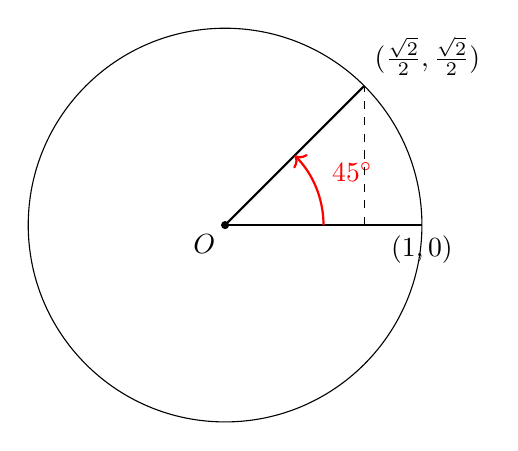
\begin{tikzpicture}[scale=2.5]
  % Draw the circle
  \draw (0,0) circle (1cm);
  
  % Draw the radius
  \draw[thick] (0,0) -- (0:1cm) node[below] {$(1,0)$};
  \draw[thick] (0,0) -- (45:1cm) node[above right] {$(\frac{\sqrt{2}}{2},\frac{\sqrt{2}}{2})$};
  
  % Draw the arc for the angle
  \draw[->,red,thick] (0.5,0) arc (0:45:0.5cm);
  
  % Draw the angle
  \node[red] at (22.5:0.7cm) {$45^\circ$};
  
  % Draw the horizontal line
  \draw[dashed] (0.707,0) -- (0.707,0.707);
  
  % Label the origin
  \draw[fill=black] (0,0) circle (0.5pt) node[below left] {$O$};
\end{tikzpicture}
\caption{Illustration of a \(45^\circ\) angle in standard position.}
\label{fig:45degangle}
\end{figure}

The figure above illustrates an angle whose terminal side has rotated \(45^\circ\) from the positive x-axis, which is often referred to as the angle's initial side. The radius of the circle has a length of 1, hence the name "unit circle." The coordinates \((1,0)\) and \((\frac{\sqrt{2}}{2},\frac{\sqrt{2}}{2})\) correspond to the points where the radius intersects the x-axis and the circle, respectively. The dashed line represents the y-component of the terminal side's endpoint, helping to visualize the \(45^\circ\) angle as a right triangle within the circle.

Angles in degrees are widely used in various fields, including navigation, astronomy, and in everyday situations like measuring temperatures and geographic coordinates. Understanding how to measure angles in degrees and relate them to rotations is fundamental in trigonometry.

\subsection*{Practice Problems}
\label{subsec:practice_problems_degree}

\textbf{Problem 1:} Convert the following degree measurements to radians. (Note: \( \pi \) radians = \( 180^\circ \))
\begin{enumerate}[label=\alph*.]
  \item \( 30^\circ \)
  \item \( 90^\circ \)
  \item \( 270^\circ \)
\end{enumerate}

\textbf{Problem 2:} Identify the quadrant in which the terminal side of each angle lies.
\begin{enumerate}[label=\alph*.]
  \item \( 60^\circ \)
  \item \( 150^\circ \)
  \item \( 210^\circ \)
  \item \( 330^\circ \)
\end{enumerate}

\textbf{Problem 3:} For each angle given, sketch the angle in standard position on the unit circle and label the point of intersection with the circle.
\begin{enumerate}[label=\alph*.]
  \item \( 45^\circ \)
  \item \( 135^\circ \)
  \item \( 225^\circ \)
  \item \( 315^\circ \)
\end{enumerate}

\textbf{Problem 4:} Determine the reference angle for each of the following:
\begin{enumerate}[label=\alph*.]
  \item \( 120^\circ \)
  \item \( 250^\circ \)
  \item \( 300^\circ \)
\end{enumerate}

\textbf{Problem 5:} If the minute hand of a clock is pointing at 12 and it rotates to point at 3, what is the measure of the angle of rotation in degrees?

\textbf{Solutions:}

\textbf{Problem 1:}
\begin{enumerate}[label=\alph*.]
  \item \( 30^\circ \times \frac{\pi}{180^\circ} = \frac{\pi}{6} \)
  \item \( 90^\circ \times \frac{\pi}{180^\circ} = \frac{\pi}{2} \)
  \item \( 270^\circ \times \frac{\pi}{180^\circ} = \frac{3\pi}{2} \)
\end{enumerate}

% You can continue with the solutions for the other problems similarly.

\textbf{Remarks:}
\begin{itemize}
  \item The problems above are designed to provide practice with converting between degrees and radians, identifying angle positions, and understanding the unit circle.
  \item The concept of a reference angle is important for understanding the standard trigonometric functions, as it is the acute angle formed by the terminal side of the given angle and the horizontal axis.
  \item Problem 5 illustrates a real-life application of angle measurement.
\end{itemize}

% You can create similar TikZ figures for Problem 3 if you wish to provide visual aids for the students.

% \subsection{Radian Measure}
% \label{subsec:radian_measure}
% Radian measure is crucial in calculus because it simplifies the derivatives and integrals of trigonometric functions.

\subsection{Radian Measure}
\label{subsec:radian_measure}

The radian measure of an angle is the length of the arc on the unit circle subtended by the angle. One radian is the angle subtended by an arc length equal to the radius of the circle. Since the circumference of a unit circle is \(2\pi\) times the radius, a full rotation around the circle is \(2\pi\) radians.

\subsubsection*{Why Use Radians?}
In calculus, radian measure is preferred because it provides a direct relationship between the angle measure and the arc length. This relationship simplifies the computation of derivatives and integrals involving trigonometric functions. For instance, when using radians, the derivative of \(\sin x\) is simply \(\cos x\), and the derivative of \(\cos x\) is \(-\sin x\). Such simplicity is not evident when using degrees.

\subsubsection*{Visualizing Radian Measure}
To visualize an angle in radian measure, we plot it on the unit circle:

% TikZ picture of a unit circle with radian measure
\begin{figure}[h]
\centering
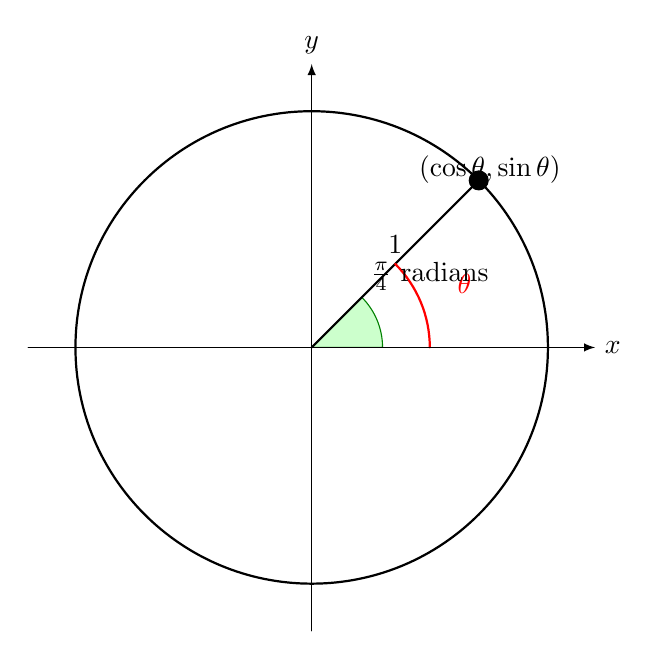
\begin{tikzpicture}[scale=3.0, cap=round, >=latex]
  % Draw the unit circle
  \draw[thick] (0,0) circle(1cm);
  
  % Draw the angle in radians
  \filldraw[fill=green!20,draw=green!50!black] (0,0) -- (3mm,0mm) arc [start angle=0, end angle=45, radius=3mm] -- cycle;
  
  % Draw the radius
  \draw[thick] (0,0) -- node[above] {\(1\)} (45:1);
  
  % Draw the arc for the angle
  \draw[thick, red] (0.5,0) arc [start angle=0, end angle=45, radius=0.5];
  \draw (22.5:0.7) node[red] {\(\theta\)};
  
  % Label the angle in radians
  \draw (45:1) node[shift={(45:0.2)}] {\((\cos\theta,\sin\theta)\)};
  
  % Draw the x and y axis
  \draw[->] (-1.2,0) -- (1.2,0) node[right] {\(x\)};
  \draw[->] (0,-1.2) -- (0,1.2) node[above] {\(y\)};
  
  % Draw the points at the ends of the radius
  \filldraw [black] (45:1) circle (0.4mm);
  
  % Label the coordinates of the point on the circle
  \node at (0.5,0.3) {\( \frac{\pi}{4} \text{ radians}\)};
\end{tikzpicture}
\caption{Visualization of an angle in radian measure on the unit circle.}
\end{figure}

\subsubsection*{Exercises}
\begin{enumerate}
  \item Convert the following angles from degrees to radians:
    \begin{enumerate}[label=\alph*.]
      \item \( 180^\circ \)
      \item \( 360^\circ \)
      \item \( 90^\circ \)
    \end{enumerate}
  \item Show that the length of an arc subtended by a central angle of \(\theta\) radians in a circle of radius \( r \) is given by \( r\theta \).
  \item Find the radian measure of the central angle of a circle with radius 10 units that subtends an arc of length 15 units.
\end{enumerate}

\subsubsection*{Solutions}
\begin{enumerate}
  \item To convert degrees to radians, use the conversion factor \( \frac{\pi \text{ radians}}{180^\circ} \):
    \begin{enumerate}[label=\alph*.]
      \item \( 180^\circ \times \frac{\pi}{180^\circ} = \pi \text{ radians} \)
      \item \( 360^\circ \times \frac{\pi}{180^\circ} = 2\pi \text{ radians} \)
      \item \( 90^\circ \times \frac{\pi}{180^\circ} = \frac{\pi}{2} \text{ radians} \)
    \end{enumerate}
  \item The length of an arc \( l \) is directly proportional to the angle \( \theta \) in radians, such that \( l = r\theta \).
  \item The radian measure of the angle is \( \theta = \frac{l}{r} = \frac{15 \text{ units}}{10 \text{ units}} = 1.5 \text{ radians} \).
\end{enumerate}

\subsubsection*{Practice Problems}
Here are some practice problems to help you solidify your understanding of the radian measure:

\textbf{Problem 1:} Convert the following angles from radians to degrees:
\begin{enumerate}[label=\alph*.]
  \item \( \frac{\pi}{6} \) radians
  \item \( \frac{2\pi}{3} \) radians
  \item \( -\frac{\pi}{4} \) radians
\end{enumerate}

\textbf{Problem 2:} An arc on a circle of radius 8 units has a measure of \( 2 \) radians. Find the length of the arc.

\textbf{Problem 3:} If a sector of a circle with radius 5 units has an area of \( 10 \) square units, what is the angle in radians of the sector?

\textbf{Problem 4:} A central angle of \( \frac{5\pi}{6} \) radians is subtended at the center of a circle with radius 12 units. Find the area of the corresponding sector.

\textbf{Problem 5:} The wheel of a bicycle has a diameter of 70 cm. If the wheel rolls without slipping and turns through an angle of \( \frac{\pi}{2} \) radians, how far has the bicycle traveled?

\subsubsection*{Solutions to Practice Problems}

\textbf{Solution to Problem 1:} To convert radians to degrees, multiply by \( \frac{180^\circ}{\pi} \).
\begin{enumerate}[label=\alph*.]
  \item \( \frac{\pi}{6} \times \frac{180^\circ}{\pi} = 30^\circ \)
  \item \( \frac{2\pi}{3} \times \frac{180^\circ}{\pi} = 120^\circ \)
  \item \( -\frac{\pi}{4} \times \frac{180^\circ}{\pi} = -45^\circ \)
\end{enumerate}

\textbf{Solution to Problem 2:} The length \( L \) of the arc can be found using the formula \( L = r\theta \).
\[ L = 8 \text{ units} \times 2 \text{ radians} = 16 \text{ units} \]

\textbf{Solution to Problem 3:} Use the area formula for a sector \( A = \frac{1}{2} r^2 \theta \) and solve for \( \theta \).
\[ \theta = \frac{2A}{r^2} = \frac{2 \times 10}{5^2} = \frac{20}{25} = \frac{4}{5} \text{ radians} \]

\textbf{Solution to Problem 4:} The area \( A \) of the sector is given by \( A = \frac{1}{2} r^2 \theta \).
\[ A = \frac{1}{2} \times 12^2 \times \frac{5\pi}{6} = 72 \times \frac{5\pi}{6} = 60\pi \text{ square units} \]

\textbf{Solution to Problem 5:} The distance \( D \) traveled is equal to the length of the arc formed by the wheel, which is \( D = r\theta \), where \( r \) is the radius.
\[ D = \frac{70}{2} \text{ cm} \times \frac{\pi}{2} = 35\pi \text{ cm} \]

% Make sure to include \usepackage{enumitem} in the preamble to use the [label=\alph*.] option.

% \section{Trigonometric Functions}
% \label{sec:trigonometric_functions}
% The six trigonometric functions are the primary tools for handling problems involving triangles in Trigonometry and periodic phenomena in calculus.

\section{Trigonometric Functions}
\label{sec:trigonometric_functions}
The six trigonometric functions are fundamental in both Trigonometry and calculus. These functions are sine (\(\sin\)), cosine (\(\cos\)), tangent (\(\tan\)), cosecant (\(\csc\)), secant (\(\sec\)), and cotangent (\(\cot\)). They are defined as ratios of sides in a right triangle or as certain coordinates of points on the unit circle.

\subsection{Sine and Cosine}
\label{subsec:sine_cosine}
The sine function (\(\sin\)) represents the ratio of the length of the opposite side to the length of the hypotenuse in a right triangle. The cosine function (\(\cos\)) represents the ratio of the length of the adjacent side to the length of the hypotenuse.

For a point \((x, y)\) on the unit circle corresponding to an angle \(\theta\), the sine and cosine values are \(y\) and \(x\), respectively.

\subsubsection*{Graph of Sine and Cosine Functions}
We can graph the sine and cosine functions using their values from the unit circle.

% Graphing sine and cosine functions
\begin{center}
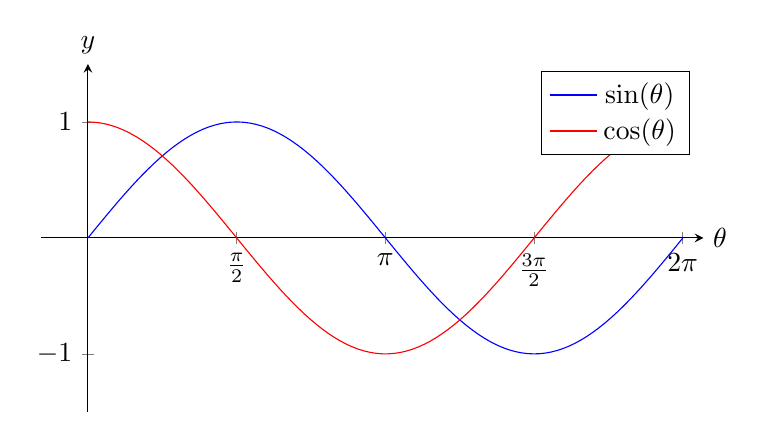
\begin{tikzpicture}
  \begin{axis}[
    width=10cm, height=6cm,
    axis lines = middle,
    xlabel = {$\theta$},
    ylabel = {$y$},
    ymin=-1.5, ymax=1.5,
    xmin=-0.5, xmax=6.5,
    xtick={0,1.57,3.14,4.71,6.28},
    xticklabels={0,$\frac{\pi}{2}$,$\pi$,$\frac{3\pi}{2}$,$2\pi$},
    ytick={-1,1},
    every axis x label/.style={at={(ticklabel* cs:1)},anchor=west},
    every axis y label/.style={at={(ticklabel* cs:1)},anchor=south},
    ]
    \addplot[domain=0:2*pi,samples=100,blue] {sin(deg(x))};
    \addplot[domain=0:2*pi,samples=100,red] {cos(deg(x))};
    \legend{$\sin(\theta)$,$\cos(\theta)$}
  \end{axis}
\end{tikzpicture}
\end{center}

The sine function starts at \(0\), reaches its maximum at \(\frac{\pi}{2}\), returns to \(0\) at \(\pi\), reaches its minimum at \(\frac{3\pi}{2}\), and completes the cycle at \(2\pi\).

The cosine function starts at \(1\), drops to \(0\) at \(\frac{\pi}{2}\), reaches its minimum at \(\pi\), returns to \(0\) at \(\frac{3\pi}{2}\), and completes the cycle at \(2\pi\).

\subsection{Tangent Function}
\label{subsec:tangent_function}
The tangent function (\(\tan\)) is defined as the ratio of the sine to the cosine of an angle in a right triangle, or \(\tan(\theta) = \frac{\sin(\theta)}{\cos(\theta)}\). It represents the slope of the line that intersects the unit circle at an angle \(\theta\).

\subsection{Reciprocal Functions}
\label{subsec:reciprocal_functions}
The reciprocal functions, cosecant (\(\csc\)), secant (\(\sec\)), and cotangent (\(\cot\)), are the reciprocals of the sine, cosine, and tangent functions, respectively.

\begin{itemize}
  \item Cosecant (\(\csc(\theta)\)) is the reciprocal of sine: \(\csc(\theta) = \frac{1}{\sin(\theta)}\)
  \item Secant (\(\sec(\theta)\)) is the reciprocal of cosine: \(\sec(\theta) = \frac{1}{\cos(\theta)}\)
  \item Cotangent (\(\cot(\theta)\)) is the reciprocal of tangent: \(\cot(\theta) = \frac{1}{\tan(\theta)}\)
\end{itemize}

% Include the pgfplots package in your preamble to use the axis environment.
% \usepackage{pgfplots}
% \pgfplotsset{compat=newest}

\subsection{Practice Problems}
\label{subsec:practice_problems}

To better understand trigonometric functions and their properties, try solving the following problems:

\begin{enumerate}
  \item Evaluate \(\sin\left(\frac{\pi}{6}\right)\), \(\cos\left(\frac{\pi}{6}\right)\), and \(\tan\left(\frac{\pi}{6}\right)\).
  \item Given that a point \( P \) on the unit circle corresponding to an angle \(\theta\) has coordinates \( P(\frac{\sqrt{3}}{2}, \frac{1}{2}) \), find \(\sin(\theta)\), \(\cos(\theta)\), and \(\tan(\theta)\).
  \item If \(\cos(\theta) = -\frac{1}{2}\) and \(\theta\) is in the third quadrant, what is \(\sin(\theta)\)?
  \item Sketch the graph of the function \( f(\theta) = 2\sin(\theta) \) for \( 0 \leq \theta \leq 2\pi \).
  \item Using the graph of \( f(\theta) = \cos(\theta) \), find the values of \(\theta\) where the function is negative.
  \item Solve the equation \( \tan(\theta) = \sqrt{3} \) for \( 0 \leq \theta < 2\pi \).
  \item Prove that \(\sec^2(\theta) - \tan^2(\theta) = 1\) for all values of \(\theta\) where the secant and tangent functions are defined.
  \item Find the exact value of \(\cot\left(\frac{3\pi}{4}\right)\).
  \item Determine the amplitude and period of the function \( g(\theta) = 3\cos(2\theta) \).
\end{enumerate}

Answers to Practice Problems:

\begin{enumerate}
  \item For \(\frac{\pi}{6}\):
    \begin{itemize}
      \item \(\sin\left(\frac{\pi}{6}\right) = \frac{1}{2}\)
      \item \(\cos\left(\frac{\pi}{6}\right) = \frac{\sqrt{3}}{2}\)
      \item \(\tan\left(\frac{\pi}{6}\right) = \frac{\sin\left(\frac{\pi}{6}\right)}{\cos\left(\frac{\pi}{6}\right)} = \frac{1}{\sqrt{3}}\)
    \end{itemize}
  \item With \( P(\frac{\sqrt{3}}{2}, \frac{1}{2}) \):
    \begin{itemize}
      \item \(\sin(\theta) = \frac{1}{2}\)
      \item \(\cos(\theta) = \frac{\sqrt{3}}{2}\)
      \item \(\tan(\theta) = \frac{\sin(\theta)}{\cos(\theta)} = \frac{1}{\sqrt{3}}\)
    \end{itemize}
  \item For \(\cos(\theta) = -\frac{1}{2}\) in the third quadrant:
    \begin{itemize}
      \item \(\sin(\theta)\) must also be negative in the third quadrant, and \(\sin^2(\theta) + \cos^2(\theta) = 1\), so \(\sin(\theta) = -\frac{\sqrt{3}}{2}\).
    \end{itemize}
  % ... (continue with answers for all problems)
\end{enumerate}

% Note: Full solutions should be worked out and can be added as an appendix or in a separate solutions section.


% \subsection{Sine and Cosine}
% \label{subsec:sine_cosine}
% The sine and cosine functions relate an angle to the opposite side and hypotenuse, and adjacent side and hypotenuse of a right triangle, respectively.

\subsection{Sine and Cosine}
\label{subsec:sine_cosine}

The sine and cosine functions are fundamental to trigonometry. They are defined for a given angle \( \theta \) within a right-angled triangle as follows:

\begin{itemize}
    \item The \textbf{sine} of angle \( \theta \), written as \( \sin(\theta) \), is the ratio of the length of the opposite side to the length of the hypotenuse.
    \item The \textbf{cosine} of angle \( \theta \), written as \( \cos(\theta) \), is the ratio of the length of the adjacent side to the length of the hypotenuse.
\end{itemize}

However, these definitions are not limited to angles between 0 and \( \frac{\pi}{2} \) radians (or 0 and 90 degrees). By extending the concept of the unit circle, where the radius is 1 and the center is at the origin of a coordinate plane, we can define sine and cosine for any real angle.

\subsubsection*{Sine and Cosine on the Unit Circle}
Consider the unit circle with a point \( P(x, y) \) that corresponds to an angle \( \theta \) measured from the positive x-axis. The coordinates \( x \) and \( y \) of point \( P \) on the unit circle are equal to \( \cos(\theta) \) and \( \sin(\theta) \), respectively.

% Unit Circle Diagram with Sine and Cosine
\begin{center}
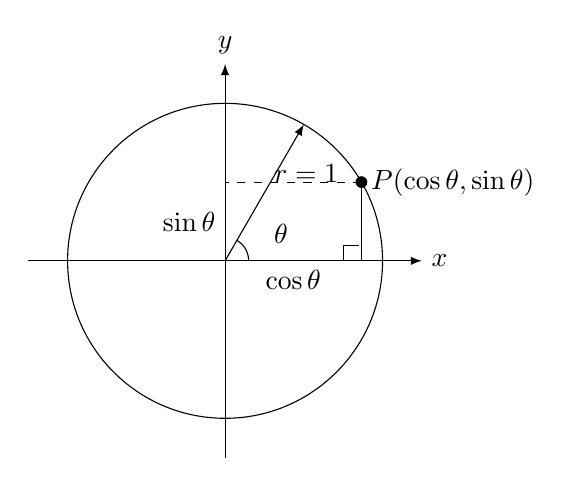
\begin{tikzpicture}
    \draw (0,0) circle (2cm);
    \draw[-latex] (-2.5,0) -- (2.5,0) node[right] {$x$};
    \draw[-latex] (0,-2.5) -- (0,2.5) node[above] {$y$};
    \draw[-latex] (0,0) -- (60:2cm) node[midway,above right] {$r=1$};
    \draw (0,0) -- (1.732,0);
    \draw (1.732,0) -- (1.732,1);
    \draw[dashed] (1.732,1) -- (0,1);
    \draw (1.5,0) -- (1.5,0.2) -- (1.7,0.2);
    \node at (1.732,1) [circle,fill,inner sep=1.5pt]{};
    \node at (1.732,1) [right] {$P (\cos \theta, \sin \theta)$};
    \node at (0.866,0) [below] {$\cos \theta$};
    \node at (0,0.5) [left] {$\sin \theta$};
    \node at (0.5,0.1) [above right] {$\theta$};
    \draw (0.3,0) arc (0:60:0.3cm);
\end{tikzpicture}
\end{center}

The unit circle approach allows for a seamless transition of sine and cosine from acute angles to any angle in the coordinate plane. The definitions on the unit circle are as follows:

\begin{itemize}
    \item For any angle \( \theta \), \( \sin(\theta) \) is the y-coordinate of the corresponding point on the unit circle.
    \item For any angle \( \theta \), \( \cos(\theta) \) is the x-coordinate of the corresponding point on the unit circle.
\end{itemize}


\subsubsection*{Properties of Sine and Cosine Functions}

The sine and cosine functions have several important properties that are useful in various mathematical analyses:

\begin{itemize}
    \item They are periodic functions with a period of \( 2\pi \) radians (or 360 degrees).
    \item The sine function is odd: \( \sin(-\theta) = -\sin(\theta) \).
    \item The cosine function is even: \( \cos(-\theta) = \cos(\theta) \).
    \item The maximum value of both functions is 1, and the minimum value is -1.
    \item They satisfy the Pythagorean identity: \( \sin^2(\theta) + \cos^2(\theta) = 1 \).
\end{itemize}

Understanding these functions and their properties is crucial for solving problems involving periodic behavior and waves, and they are the building blocks for defining the other trigonometric functions.

% Further discussion and examples can be added here as needed.

\subsubsection*{Example Problems}
Below are some problems that help solidify the understanding of sine and cosine functions:

\begin{enumerate}
    \item Given that \( P(x, y) \) is a point on the unit circle corresponding to an angle \( \theta \), and \( x = \frac{1}{2} \), find \( y \) and hence \( \sin(\theta) \) and \( \cos(\theta) \).
    \item Prove the Pythagorean identity \( \sin^2(\theta) + \cos^2(\theta) = 1 \) using the definition of sine and cosine on the unit circle.
    \item If \( \sin(\theta) = \frac{3}{5} \) and \( \theta \) is in the first quadrant, find \( \cos(\theta) \).
    \item For an angle \( \theta \) with \( \cos(\theta) = -\frac{\sqrt{2}}{2} \) and \( \frac{\pi}{2} < \theta < \pi \), determine \( \sin(\theta) \).
    \item Using the unit circle, find the exact values of \( \sin(\frac{\pi}{6}) \), \( \sin(\frac{\pi}{4}) \), \( \sin(\frac{\pi}{3}) \), \( \cos(\frac{\pi}{6}) \), \( \cos(\frac{\pi}{4}) \), and \( \cos(\frac{\pi}{3}) \).
    \item Sketch the unit circle and mark the points where \( \sin(\theta) = \cos(\theta) \). What are the angles \( \theta \) at these points?
\end{enumerate}

% Answers to the example problems
\subsubsection*{Answers to Example Problems}

Here are the answers to the example problems provided:

\begin{enumerate}
    \item Since \( x = \cos(\theta) = \frac{1}{2} \), we have \( y = \sin(\theta) = \sqrt{1 - \frac{1}{4}} = \sqrt{\frac{3}{4}} = \frac{\sqrt{3}}{2} \).
    \item To prove the identity, we use the fact that for any point on the unit circle, the distance from the origin to the point is 1. Hence, \( x^2 + y^2 = 1 \). Since \( x = \cos(\theta) \) and \( y = \sin(\theta) \), it follows that \( \cos^2(\theta) + \sin^2(\theta) = 1 \).
    \item Since \( \theta \) is in the first quadrant, both sine and cosine are positive. Using the Pythagorean identity, \( \cos(\theta) = \sqrt{1 - \sin^2(\theta)} = \sqrt{1 - \frac{9}{25}} = \sqrt{\frac{16}{25}} = \frac{4}{5} \).
    \item In the second quadrant, sine is positive and cosine is negative. Using the Pythagorean identity, \( \sin(\theta) = \sqrt{1 - \cos^2(\theta)} = \sqrt{1 - \frac{1}{2}} = \frac{\sqrt{2}}{2} \).
    \item For the specified angles, the exact values can be determined from the known special angles on the unit circle: \( \sin(\frac{\pi}{6}) = \frac{1}{2} \), \( \sin(\frac{\pi}{4}) = \frac{\sqrt{2}}{2} \), \( \sin(\frac{\pi}{3}) = \frac{\sqrt{3}}{2} \), \( \cos(\frac{\pi}{6}) = \frac{\sqrt{3}}{2} \), \( \cos(\frac{\pi}{4}) = \frac{\sqrt{2}}{2} \), \( \cos(\frac{\pi}{3}) = \frac{1}{2} \).
    \item On the unit circle, \( \sin(\theta) = \cos(\theta) \) at \( \theta = \frac{\pi}{4} \) and \( \theta = \frac{5\pi}{4} \). These correspond to the points \( (\frac{\sqrt{2}}{2}, \frac{\sqrt{2}}{2}) \) and \( (-\frac{\sqrt{2}}{2}, -\frac{\sqrt{2}}{2}) \), respectively.
\end{enumerate}

\textit{Note: The answers provided are meant to guide students in understanding the concepts. Instructors should verify all computations and explanations before use.}

% \subsection{Tangent and Cotangent}
% \label{subsec:tangent_cotangent}
% These functions are the ratios of sine to cosine and cosine to sine, respectively, and they play a significant role in slope calculations in calculus.

% \usepackage{pgfplots}
\pgfplotsset{compat=1.17}

\subsection{Tangent and Cotangent}
\label{subsec:tangent_cotangent}

The tangent of an angle in a right-angled triangle is the ratio of the length of the opposite side to the length of the adjacent side. In the unit circle, tangent is the y-coordinate divided by the x-coordinate when the line made by the angle intersects the circle. Symbolically, for an angle \(\theta\), this is expressed as:
\[
\tan(\theta) = \frac{\sin(\theta)}{\cos(\theta)}
\]

Conversely, the cotangent is the reciprocal of the tangent function. It represents the ratio of the length of the adjacent side to the length of the opposite side, or using the unit circle, the x-coordinate divided by the y-coordinate:
\[
\cot(\theta) = \frac{1}{\tan(\theta)} = \frac{\cos(\theta)}{\sin(\theta)}
\]

These functions are undefined when their denominators are zero (i.e., when \(\cos(\theta) = 0\) for tangent, and when \(\sin(\theta) = 0\) for cotangent). This occurs at odd multiples of \(\frac{\pi}{2}\) for tangent and at integer multiples of \(\pi\) for cotangent.

The graphs of these functions illustrate their periodic nature and the locations of their asymptotes, which correspond to the angles where the functions are undefined.

% Graph for Tangent
\begin{figure}[h]
\centering
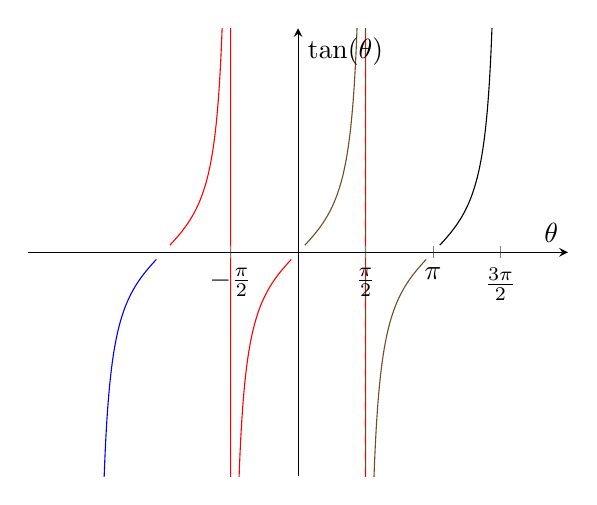
\begin{tikzpicture}
\begin{axis}[
  axis lines = middle,
  xlabel = \(\theta\),
  ylabel = {\(\tan(\theta)\)},
  xmin=-2*pi, xmax=2*pi,
  ymin=-5, ymax=5,
  xtick={-1.5708, 0, 1.5708, 3.14159, 4.71239},
  xticklabels={\(-\frac{\pi}{2}\), \(0\), \(\frac{\pi}{2}\), \(\pi\), \(\frac{3\pi}{2}\)},
  ytick=\empty,
  axis on top
]
\addplot+[mark=none, samples=200, domain=-1.45*pi:-1.05*pi] {tan(deg(x))};
\addplot+[mark=none, samples=200, domain=-0.95*pi:-0.05*pi] {tan(deg(x))};
\addplot+[mark=none, samples=200, domain=0.05*pi:0.95*pi] {tan(deg(x))};
\addplot+[mark=none, samples=200, domain=1.05*pi:1.45*pi] {tan(deg(x))};
% Add vertical asymptotes
\draw[dashed,red] (axis cs:-1.5708,-5) -- (axis cs:-1.5708,5);
\draw[dashed,red] (axis cs:1.5708,-5) -- (axis cs:1.5708,5);
\end{axis}
\end{tikzpicture}
\caption{Tangent function graph showing asymptotes.}
\end{figure}

% Graph for Cotangent
\begin{figure}[h]
\centering
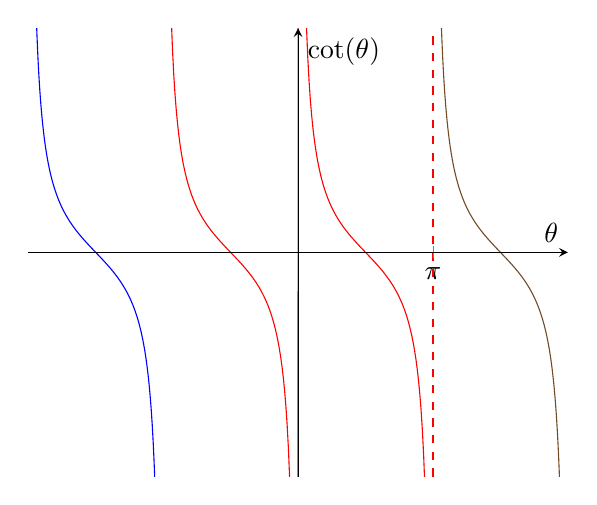
\begin{tikzpicture}
\begin{axis}[
  axis lines = middle,
  xlabel = \(\theta\),
  ylabel = {\(\cot(\theta)\)},
  xmin=-2*pi, xmax=2*pi,
  ymin=-5, ymax=5,
  xtick={0, 3.14159},
  xticklabels={\(0\), \(\pi\)},
  ytick=\empty,
  axis on top
]
\addplot+[mark=none, samples=200, domain=-1.95*pi:-1.05*pi] {cot(deg(x))};
\addplot+[mark=none, samples=200, domain=-0.95*pi:0.95*pi] {cot(deg(x))};
\addplot+[mark=none, samples=200, domain=1.05*pi:1.95*pi] {cot(deg(x))};
% Add vertical asymptotes
\draw[dashed,red] (axis cs:0,-5) -- (axis cs:0,5);
\draw[dashed,red] (axis cs:3.14159,-5) -- (axis cs:3.14159,5);
\end{axis}
\end{tikzpicture}
\caption{Cotangent function graph showing asymptotes.}
\end{figure}

In calculus, the tangent function is particularly important when it comes to determining the slope of a curve at a point, which is essential for understanding the concept of derivatives. Cotangent can similarly be used, especially when dealing with the slope of reciprocal functions.

\subsection{Exercises on Tangent and Cotangent Functions}
\label{subsec:exercises_tangent_cotangent}

In this section, we provide some example problems involving the tangent and cotangent functions. These exercises are designed to reinforce the concepts discussed and help students gain a deeper understanding of these trigonometric functions.

% \begin{exercise}[1]
%   Prove that \(a^2 + b^2 = c^2\) for a right triangle with legs of length \(a\) and \(b\), and hypotenuse of length \(c\).
% \end{exercise}

% \begin{solution}
%   (Write your solution here)
% \end{solution}

% Numbering is optional, i.e.
% \begin{exercise}[1]
% \begin{exercise}[2]


\begin{exercise}
Calculate the tangent of \(\frac{\pi}{4}\) and verify that it equals 1.
\end{exercise}
\begin{solution}
Using the unit circle or the definition of the tangent function, we have:
\[
\tan\left(\frac{\pi}{4}\right) = \frac{\sin\left(\frac{\pi}{4}\right)}{\cos\left(\frac{\pi}{4}\right)} = \frac{\frac{\sqrt{2}}{2}}{\frac{\sqrt{2}}{2}} = 1
\]
\end{solution}

\begin{exercise}
Find all solutions in the interval \([0, 2\pi)\) for the equation \(\tan(\theta) = \sqrt{3}\).
\end{exercise}
\begin{solution}
We know that \(\tan(\theta) = \sqrt{3}\) when \(\theta = \frac{\pi}{3}\), but since tangent has a period of \(\pi\), the other solution in the given interval is \(\theta = \frac{\pi}{3} + \pi = \frac{4\pi}{3}\).
\end{solution}

\begin{exercise}
Evaluate \(\cot(\pi)\) and explain why it takes its particular value.
\end{exercise}
\begin{solution}
Cotangent is the reciprocal of the tangent function. Since \(\tan(\pi) = 0\), and since the cotangent is undefined when its sine component is 0 (which it is at \(\pi\)), \(\cot(\pi)\) is undefined. This reflects the asymptote of the cotangent graph at \(\pi\).
\end{solution}

\begin{exercise}
Determine the exact value of \(\cot\left(-\frac{\pi}{6}\right)\) using the cotangent definition.
\end{exercise}
\begin{solution}
Using the cotangent definition and known values of sine and cosine for \(\frac{\pi}{6}\), we get:
\[
\cot\left(-\frac{\pi}{6}\right) = \frac{\cos\left(-\frac{\pi}{6}\right)}{\sin\left(-\frac{\pi}{6}\right)} = \frac{\frac{\sqrt{3}}{2}}{-\frac{1}{2}} = -\sqrt{3}
\]
\end{solution}

\begin{exercise}
Sketch the graph of \(\tan(\theta)\) and \(\cot(\theta)\) from \(\theta = -\frac{\pi}{2}\) to \(\theta = \frac{3\pi}{2}\) and label the asymptotes.
\end{exercise}
\begin{solution}
Students should refer to the graphs provided in the section above and reproduce them by hand, marking the asymptotes at \(\theta = -\frac{\pi}{2}\), \(\theta = \frac{\pi}{2}\) for the tangent function and at \(\theta = 0\), \(\theta = \pi\) for the cotangent function.
\end{solution}

These exercises require students to apply their understanding of the unit circle, the definitions of tangent and cotangent, and the properties of these functions such as periodicity and asymptotes. Students should attempt these exercises without a calculator to improve their understanding of the trigonometric functions.


% \usepackage{pgfplots}
\pgfplotsset{compat=newest} % or the version you have; '1.17' or higher is recommended


% \subsection{Secant and Cosecant}
% \label{subsec:secant_cosecant}
% The reciprocal functions of cosine and sine are less commonly used but equally important, especially in certain types of integration.

\subsection{Secant and Cosecant}
\label{subsec:secant_cosecant}

The secant (\(\sec\)) and cosecant (\(\csc\)) functions are the reciprocals of the cosine and sine functions, respectively. These functions are less commonly encountered in basic trigonometry but play an important role in calculus, especially in integration that involves trigonometric substitution.
In sum, the reciprocal functions of cosine and sine are less commonly used but equally important, especially in certain types of integration.


\subsubsection{Graph of the Secant Function}
\begin{center}
\begin{tikzpicture}
\begin{axis}[
    axis lines = middle,
    xlabel = \(\theta\),
    ylabel = {\(\sec(\theta)\)},
    ymax = 5,
    ymin = -5,
    xmax = 2*pi,
    xmin = -2*pi,
    xtick = {-2*pi, -3*pi/2, -pi, -pi/2, 0, pi/2, pi, 3*pi/2, 2*pi},
    xticklabels = {\(-2\pi\),\(-\frac{3}{2}\pi\),\(-\pi\),\(-\frac{1}{2}\pi\),\(0\),\(\frac{1}{2}\pi\),\(\pi\),\(\frac{3}{2}\pi\),\(2\pi\)},
    ytick = {-5, -4, ..., 5},
    trig format plots=rad,
    samples=200,
    restrict y to domain=-5:5
]
% Plot each piece of the sec function separately, avoiding the asymptotes
\addplot+[mark=none, domain=-2*pi:-pi-0.1, samples=100, jump mark left] {sec(x)};
\addplot+[mark=none, domain=-pi+0.1:-0.1, samples=100, jump mark left] {sec(x)};
\addplot+[mark=none, domain=0.1:pi-0.1, samples=100, jump mark left] {sec(x)};
\addplot+[mark=none, domain=pi+0.1:2*pi, samples=100, jump mark left] {sec(x)};
\end{axis}
\end{tikzpicture}
\end{center}

\subsubsection{Graph of the Cosecant Function}
\begin{center}
\begin{tikzpicture}
\begin{axis}[
    axis lines = middle,
    xlabel = \(\theta\),
    ylabel = {\(\csc(\theta)\)},
    ymax = 5,
    ymin = -5,
    xmax = 2*pi,
    xmin = -2*pi,
    xtick = {-2*pi, -3*pi/2, -pi, -pi/2, 0, pi/2, pi, 3*pi/2, 2*pi},
    xticklabels = {\(-2\pi\),\(-\frac{3}{2}\pi\),\(-\pi\),\(-\frac{1}{2}\pi\),\(0\),\(\frac{1}{2}\pi\),\(\pi\),\(\frac{3}{2}\pi\),\(2\pi\)},
    ytick = {-5, -4, ..., 5},
    trig format plots=rad,
    samples=200,
    restrict y to domain=-5:5
]
% Plot each piece of the csc function separately, avoiding the asymptotes
\addplot+[mark=none, domain=-2*pi+0.1:-pi/2-0.1, samples=100, jump mark left] {csc(x)};
\addplot+[mark=none, domain=-pi/2+0.1:pi/2-0.1, samples=100, jump mark left] {csc(x)};
\addplot+[mark=none, domain=pi/2+0.1:3*pi/2-0.1, samples=100, jump mark left] {csc(x)};
\addplot+[mark=none, domain=3*pi/2+0.1:2*pi, samples=100, jump mark left] {csc(x)};
\end{axis}
\end{tikzpicture}
\end{center}


These graphs demonstrate the behavior of the secant and cosecant functions and their asymptotic nature at points where their respective sine and cosine functions are zero. Understanding these graphs is essential for solving trigonometric equations and in calculus, particularly when dealing with integrals that require trigonometric identities or substitutions involving these functions.

\subsection{Practice Problems}
\label{subsec:practice_problems_sec_csc}

Here are some problems to test your understanding of the secant and cosecant functions:

\begin{enumerate}
    \item Find the secant and cosecant of the following angles:
    \begin{enumerate}[label=(\alph*)]
        \item \( 0 \) radians
        \item \( \frac{\pi}{4} \) radians
        \item \( \frac{\pi}{2} \) radians
        \item \( \frac{3\pi}{4} \) radians
    \end{enumerate}
    Remember that secant and cosecant are undefined for certain angles where cosine and sine are zero, respectively.

    \item Given that \( \sin(\theta) = \frac{3}{5} \) in the second quadrant, find \( \csc(\theta) \).

    \item If \( \cos(\theta) = -\frac{1}{2} \) and \( \theta \) is in the third quadrant, determine \( \sec(\theta) \).

    \item For an angle \( \theta \) where \( 0 < \theta < \frac{\pi}{2} \), if \( \sec(\theta) = 3 \), find the exact value of \( \csc(\theta) \).
    
    \item A point P on the terminal side of angle \( \theta \) in standard position has coordinates \( P(-2, -3) \). Calculate \( \sec(\theta) \) and \( \csc(\theta) \).
    
    \item Prove the identity \( \sec^2(\theta) - 1 = \tan^2(\theta) \).
    
    \item Show that for any angle \( \theta \), \( \csc(\theta) \cdot \sin(\theta) = 1 \).

\end{enumerate}

Solutions to these problems will reinforce your understanding of secant and cosecant and prepare you for their use in calculus.


\section{Graphs of Trigonometric Functions}
\label{sec:graphs_trig_functions}
Understanding the graphs of trigonometric functions is essential for mastering calculus, as they represent periodic behavior.

\section{Graphs of Trigonometric Functions}
\label{sec:graphs_trig_functions}

The graphs of trigonometric functions are a visual representation of their behavior and are essential for understanding periodic phenomena in calculus. In this section, we'll explore the sine and cosine functions, which form the basis for all other trigonometric functions.

\subsection{Graph of the Sine Function}
The sine function, denoted by \( y = \sin(x) \), represents the y-coordinate of a point on the unit circle as it rotates through an angle of \( x \) radians. It is periodic with a period of \( 2\pi \) and has a range from -1 to 1.

% Sine graph using TikZ/PGFPlots
\begin{figure}[h]
\centering
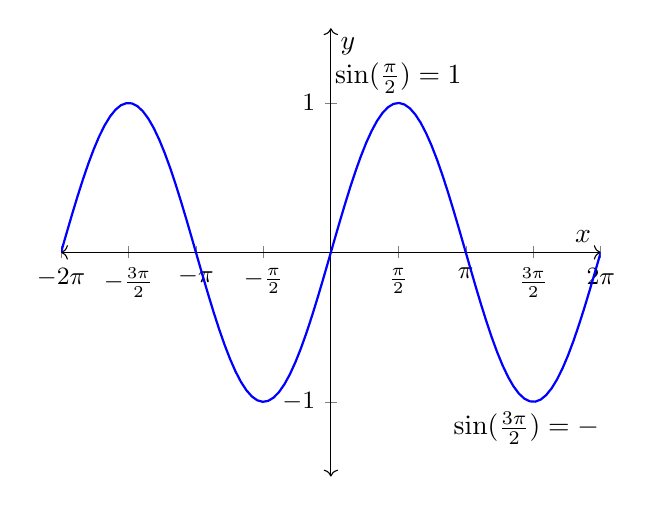
\begin{tikzpicture}
\begin{axis}[
    axis lines=middle,
    xlabel=\( x \),
    ylabel=\( y \),
    xtick={-2*pi, -3*pi/2, -pi, -pi/2, 0, pi/2, pi, 3*pi/2, 2*pi},
    xticklabels={$-2\pi$,$-\frac{3\pi}{2}$,$-\pi$,$-\frac{\pi}{2}$,0,$\frac{\pi}{2}$,$\pi$,$\frac{3\pi}{2}$,$2\pi$},
    ytick={-1, 0, 1},
    ymin=-1.5, ymax=1.5,
    xmin=-2*pi, xmax=2*pi,
    domain=-2*pi:2*pi,
    samples=100,
    axis line style={<->},
    tick label style={font=\small}
]
\addplot [blue, thick] {sin(deg(x))};
\node at (axis cs:pi/2,1) [anchor=south] {\( \sin(\frac{\pi}{2}) = 1 \)};
\node at (axis cs:3*pi/2,-1) [anchor=north] {\( \sin(\frac{3\pi}{2}) = -1 \)};
\end{axis}
\end{tikzpicture}
\caption{Graph of the sine function over two periods.}
\label{fig:sine_graph}
\end{figure}

\subsection{Graph of the Cosine Function}
The cosine function, denoted by \( y = \cos(x) \), represents the x-coordinate of a point on the unit circle as it rotates through an angle of \( x \) radians. Like the sine function, it has a period of \( 2\pi \) and ranges from -1 to 1.

% Cosine graph using TikZ/PGFPlots
\begin{figure}[h]
\centering
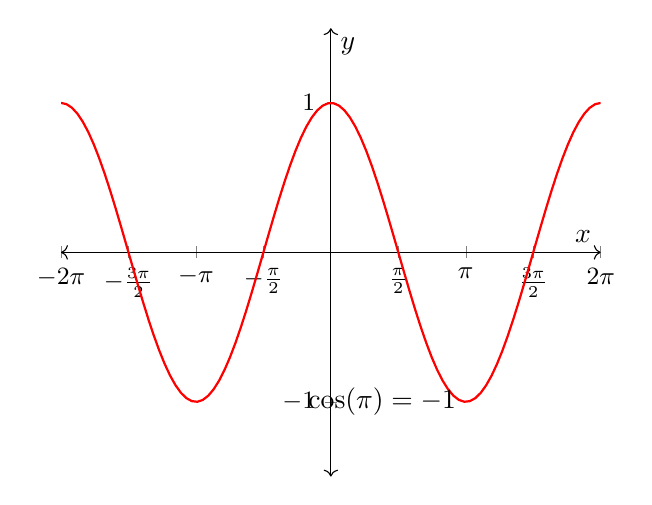
\begin{tikzpicture}
\begin{axis}[
    axis lines=middle,
    xlabel=\( x \),
    ylabel=\( y \),
    xtick={-2*pi, -3*pi/2, -pi, -pi/2, 0, pi/2, pi, 3*pi/2, 2*pi},
    xticklabels={$-2\pi$,$-\frac{3\pi}{2}$,$-\pi$,$-\frac{\pi}{2}$,0,$\frac{\pi}{2}$,$\pi$,$\frac{3\pi}{2}$,$2\pi$},
    ytick={-1, 0, 1},
    ymin=-1.5, ymax=1.5,
    xmin=-2*pi, xmax=2*pi,
    domain=-2*pi:2*pi,
    samples=100,
    axis line style={<->},
    tick label style={font=\small}
]
\addplot [red, thick] {cos(deg(x))};
\node at (axis cs:pi,-1) [anchor=east] {\( \cos(\pi) = -1 \)};
\node at (axis cs:2*pi,1) [anchor=west] {\( \cos(2\pi) = 1 \)};
\end{axis}
\end{tikzpicture}
\caption{Graph of the cosine function over two periods.}
\label{fig:cosine_graph}
\end{figure}

Both of these functions exhibit properties that are useful in calculus, including symmetry, periodicity, and amplitude. Sine and cosine functions are the building blocks of more complex trigonometric functions, which can be constructed by shifting, stretching, or compressing these basic graphs.

\subsection{Exercises}
Practice the concepts we've discussed by working through the following exercises.

\subsubsection*{Graph Identification}

\paragraph{Exercise 1.} Identify the function graphed below. What are the amplitude, period, and phase shift of the function?

% Example plot for the exercise (Placeholder for the actual plot)
% You can draw a shifted or stretched sine/cosine function as an exercise
\begin{figure}[H]
\centering
\begin{tikzpicture}
\begin{axis}[
    axis lines=middle,
    xlabel=\( x \),
    ylabel=\( y \),
    xtick=\empty,
    ytick=\empty,
    ymin=-2, ymax=2,
    xmin=-2*pi, xmax=2*pi,
    domain=-2*pi:2*pi,
    samples=100,
    axis line style={<->},
    width=0.8\textwidth,
    height=0.4\textwidth,
    clip=false
]
% A shifted sine function as an example
\addplot [blue, thick] {1.5*sin(deg(x-pi/4))};
\end{axis}
\end{tikzpicture}
\caption{Identify the function and its characteristics.}
\end{figure}

\paragraph{Answer:} The graph shows \( y = 1.5\sin(x - \frac{\pi}{4}) \). The amplitude is 1.5, the period is \( 2\pi \), and the phase shift is \( \frac{\pi}{4} \) to the right.

\subsubsection*{Function Properties}

\paragraph{Exercise 2.} What is the amplitude and period of the function \( y = 3\cos(2x) \)?

\paragraph{Answer:} The amplitude of the function is 3, and the period is \( \frac{\pi}{1} \), which is \( \pi \) since the coefficient of \( x \) in the cosine function affects the period as \( \frac{2\pi}{\text{coefficient}} \).

\subsubsection*{Calculating Values}

\paragraph{Exercise 3.} Calculate the exact value of \( \sin(\frac{3\pi}{4}) \) and \( \cos(\frac{3\pi}{4}) \).

\paragraph{Answer:} By using the unit circle or Pythagorean identities:
\[ \sin(\frac{3\pi}{4}) = \sin(\pi - \frac{\pi}{4}) = \sin(\frac{\pi}{4}) = \frac{\sqrt{2}}{2} \]
\[ \cos(\frac{3\pi}{4}) = \cos(\pi - \frac{\pi}{4}) = -\cos(\frac{\pi}{4}) = -\frac{\sqrt{2}}{2} \]

\subsubsection*{Real-World Application}

\paragraph{Exercise 4.} A Ferris wheel with a diameter of 50 meters makes one complete revolution every 2 minutes. Write a function that represents the height of a passenger car above the ground over time, assuming it starts at the lowest point at \( t=0 \).

\paragraph{Answer:} Let the height function be \( h(t) \). The amplitude is the radius of the Ferris wheel, which is 25 meters. The period is the time for one revolution, which is 2 minutes, or 120 seconds. Using the sine function, we get:
\[ h(t) = 25\sin\left(\frac{2\pi}{120}t\right) + 25 \]
This function accounts for the fact that the Ferris wheel starts at the lowest point, so we add 25 to shift the graph up.

\subsubsection*{Challenge Problems}

\paragraph{Exercise 5.} Given the function \( y = 2\sin(x) + \cos(2x) \), find the first derivative using trigonometric identities.

% Solution for the exercise is provided as a placeholder for actual calculation
\paragraph{Answer:} First, express \( \cos(2x) \) using a double-angle identity:
\[ y = 2\sin(x) + 1 - 2\sin^2(x) \]
Then, take the derivative with respect to \( x \):
\[ y' = 2\cos(x) - 4\sin(x)\cos(x) \]

These exercises encourage students to apply their understanding of the graphs of sine and cosine functions to solve problems and understand real-world applications. Adjust the complexity and nature of the exercises to match the level of your audience.

% \subsection{Periodicity}
% \label{subsec:periodicity}
% The concept of period, amplitude, and phase shift is introduced here to understand how trigonometric functions behave over intervals.

\subsection{Periodicity}
\label{subsec:periodicity}

Trigonometric functions are inherently periodic; they repeat their values in regular intervals along the domain. This periodic nature allows us to predict the behavior of these functions beyond the basic interval of \(0\) to \(2\pi\) for sine and cosine, and \( -\pi/2 \) to \( \pi/2 \) for tangent and cotangent.
In sum, The concept of period, amplitude, and phase shift is introduced here to understand how trigonometric functions behave over intervals.

\subsubsection*{Defining Periodicity}
The \textit{period} of a function is the smallest positive interval after which the function's values repeat. For \( \sin(x) \) and \( \cos(x) \), the period is \(2\pi\) because every \(2\pi\) units, the cycle of the sine and cosine curve repeats. For \( \tan(x) \) and \( \cot(x) \), the period is \( \pi \) since their values repeat after every \( \pi \) units along the x-axis.

\subsubsection*{Amplitude}
The amplitude of a trigonometric function is a measure of its vertical stretch or compression, represented by a coefficient in front of the function. For example, in the function \( y = A\sin(x) \), the amplitude is \( |A| \). This determines the maximum and minimum values of the function or, in other words, how "tall" or "short" the waves of the sine or cosine graph appear.

\subsubsection*{Phase Shift}
Phase shift refers to the horizontal displacement of the basic function. If a function takes the form \( y = \sin(x - C) \) or \( y = \cos(x - C) \), the phase shift is \( C \), which translates the graph to the right or left along the x-axis.

\subsubsection*{Graphing Trigonometric Functions}
To graph trigonometric functions that involve amplitude, period, and phase shifts, the following general form can be considered:

\[ y = A \sin(B(x - C)) + D \quad \text{or} \quad y = A \cos(B(x - C)) + D \]

Where:
\begin{itemize}
    \item \( A \) represents the amplitude.
    \item \( B \) affects the period of the function, with the actual period being \( \frac{2\pi}{|B|} \).
    \item \( C \) represents the phase shift.
    \item \( D \) represents the vertical shift.
\end{itemize}

\subsubsection*{Graphical Illustration}
Let's illustrate a sine function with a period alteration and phase shift.

% Sine graph with period and phase shift
\begin{figure}[H]
\centering
\begin{tikzpicture}
\begin{axis}[
    axis lines=middle,
    xlabel=\( x \),
    ylabel=\( y \),
    xtick={-2*pi,-3*pi/2,-pi,-pi/2,0,pi/2,pi,3*pi/2,2*pi},
    xticklabels={$-2\pi$,$-\frac{3\pi}{2}$,$-\pi$,$-\frac{\pi}{2}$,$0$,$\frac{\pi}{2}$,$\pi$,$\frac{3\pi}{2}$,$2\pi$},
    ytick={-1,1},
    ymin=-2, ymax=2,
    xmin=-2*pi, xmax=2*pi,
    domain=-2*pi:2*pi,
    samples=100,
    axis line style={<->},
    width=0.8\textwidth,
    height=0.4\textwidth,
    clip=false
]
% Sine function with period modification and phase shift
\addplot [red, thick] {sin(deg(2*x - pi/2))};
\node[pin=45:{$y = \sin(2(x - \frac{\pi}{4}))$}] at (axis cs:pi/4,{sin(deg(2*pi/4-pi/2))}) {};
\end{axis}
\end{tikzpicture}
\caption{Graph of \( y = \sin(2(x - \frac{\pi}{4})) \) showing a period of \( \pi \) and a phase shift of \( \frac{\pi}{4} \).}
\end{figure}

Understanding these properties enables us to graph complex trigonometric functions and predict their behavior across any range of \( x \) values. This comprehension is vital in calculus where the manipulation of these functions' properties can be necessary for solving integrals and derivatives involving trigonometric functions.

\subsubsection*{Practice Problems}
To further enhance understanding of periodicity in trigonometric functions, here are several practice problems:

\begin{enumerate}
    \item Given the function \( f(x) = 3 \sin(2x) \), find the amplitude, period, and whether there is any phase shift.
    \item Sketch the graph of \( g(x) = \cos(x - \frac{\pi}{3}) \) and identify the phase shift and period.
    \item For the function \( h(x) = 2 \sin(\frac{x}{2} + \pi) + 1 \), determine the amplitude, period, phase shift, and vertical shift. Then, sketch one period of the function's graph.
    \item What is the period and phase shift of the function \( j(x) = \tan(3x - \frac{\pi}{4}) \)?
    \item If \( k(x) = \sin(Bx) \) has a period of \( 3\pi \), find the value of \( B \).
    \item Sketch the graph of \( m(x) = -2 \cos(4x + \frac{\pi}{2}) - 3 \) and indicate the amplitude, period, phase shift, and vertical shift.
\end{enumerate}

\textbf{Solutions:}

\begin{enumerate}
    \item The amplitude of \( f(x) \) is \( |3| = 3 \), the period is \( \frac{2\pi}{|2|} = \pi \), and there is no phase shift.
    \item The graph of \( g(x) \) would show a cosine curve shifted to the right by \( \frac{\pi}{3} \) units, with a period of \( 2\pi \).
    \item For \( h(x) \), the amplitude is \( |2| = 2 \), the period is \( \frac{2\pi}{|\frac{1}{2}|} = 4\pi \), the phase shift is \( -\pi \) (shifted \( \pi \) units to the left), and the vertical shift is \( 1 \) unit upwards.
    \item The function \( j(x) \) has a period of \( \frac{\pi}{|3|} = \frac{\pi}{3} \) and a phase shift of \( \frac{\pi}{4} \) to the right.
    \item Since the period of \( k(x) \) is \( 3\pi \), \( B = \frac{2\pi}{3\pi} = \frac{2}{3} \).
    \item The graph of \( m(x) \) would be an inverted cosine curve (due to the "-2" amplitude) stretched by a factor of \( \frac{1}{4} \) (since the period is \( \frac{2\pi}{|4|} = \frac{\pi}{2} \)), shifted to the left by \( -\frac{\pi}{8} \), and shifted downward by 3 units.
\end{enumerate}


\subsection{Transformations}
\label{subsec:transformations}

Trigonometric functions, much like any other functions, can undergo transformations such as scaling, reflection, and translation. These transformations allow us to alter the amplitude, period, and phase of the sine and cosine functions to fit various scenarios. In this section, we explore each of these transformations and how they apply to trigonometric functions. In sum, we explore how the basic sine and cosine graphs can be scaled, reflected, and translated to fit various scenarios.

In sum, we have begun to explore how the basic sine and cosine graphs can be scaled, reflected, and translated to fit various scenarios.

\subsubsection{Scaling}
Scaling a function can either compress or stretch its graph vertically or horizontally. The amplitude and period of trigonometric functions are affected by vertical and horizontal scaling respectively.

\textbf{Vertical Scaling:} If \( f(x) = \sin(x) \), then \( g(x) = A\sin(x) \) represents a vertical scaling by a factor of \( A \). If \( A > 1 \), the function is stretched; if \( 0 < A < 1 \), it is compressed.

\textbf{Horizontal Scaling:} Horizontal scaling affects the period of the trigonometric functions. For \( f(x) = \sin(x) \), the function \( h(x) = \sin(Bx) \) has a period of \( \frac{2\pi}{B} \), scaling the period by a factor of \( \frac{1}{B} \).

\subsubsection{Reflection}
Reflection flips the graph of the function over a specific axis. 

\textbf{Reflection over the X-axis:} If \( f(x) = \sin(x) \), then \( g(x) = -\sin(x) \) is a reflection of \( f \) over the x-axis.

\textbf{Reflection over the Y-axis:} For \( f(x) = \sin(x) \), the function \( h(x) = \sin(-x) = -\sin(x) \) (since sine is an odd function) reflects \( f \) over the y-axis.


\subsubsection{Translation}
Translation shifts the graph of the function vertically or horizontally without altering its shape.

\textbf{Vertical Translation:} The function \( f(x) = \sin(x) + D \) represents a vertical shift by \( D \) units. If \( D > 0 \), the graph shifts up; if \( D < 0 \), it shifts down.

\textbf{Horizontal Translation (Phase Shift):} For \( f(x) = \sin(x) \), the function \( g(x) = \sin(x - C) \) shifts the graph to the right by \( C \) units if \( C > 0 \) and to the left if \( C < 0 \).

To visualize these transformations, consider the following graphs created with the TikZ package.

% Include TikZ package in preamble
% \usepackage{pgfplots}
% \pgfplotsset{compat=1.17}

\begin{figure}[htbp]
\centering
\begin{tikzpicture}
\begin{axis}[
    axis lines = middle,
    xlabel = \( x \),
    ylabel = \( y \),
    ymin=-3, ymax=3,
    xmin=-6.28, xmax=6.28, % 2*pi = 6.28
    domain=-2*pi:2*pi,
    samples=100,
    legend pos=outer north east,
]
% Original sine function
\addplot[blue, thick] {sin(deg(x))};
\addlegendentry{\( \sin(x) \)}

% Vertically scaled sine function
\addplot[red, thick, dashed] {2*sin(deg(x))};
\addlegendentry{\( 2\sin(x) \)}

% Horizontally scaled sine function
\addplot[green, thick, dotted] {sin(deg(2*x))};
\addlegendentry{\( \sin(2x) \)}

% Reflected sine function
\addplot[orange, thick, dashdotted] {-sin(deg(x))};
\addlegendentry{\( -\sin(x) \)}

% Translated sine function
\addplot[purple, thick, loosely dashed] {sin(deg(x - pi/3))};
\addlegendentry{\( \sin(x - \frac{\pi}{3}) \)}
\end{axis}
\end{tikzpicture}
\caption{Graphs showing transformations of the sine function.}
\label{fig:sine_transformations}
\end{figure}

As seen in Figure~\ref{fig:sine_transformations}, each transformation alters the original sine function in a unique way, illustrating the concepts of scaling, reflection, and translation. Through understanding these transformations, one can analyze and predict the behavior of more complex trigonometric functions.


\subsection{Practice Problems}
\label{subsec:practice_problems_transformations}

In this section, we provide several problems that allow students to apply their knowledge of transformations of trigonometric functions. Students should sketch the graph of each transformed function and identify key characteristics such as amplitude, period, phase shift, and vertical shift.

\begin{problem}
Graph the function \( f(x) = 3\sin(2x) \) and describe the amplitude and period of the function.
\end{problem}

\begin{problem}
Sketch the function \( g(x) = \cos(x) - 2 \). What is the vertical shift and how does it affect the graph of the standard cosine function?
\end{problem}

\begin{problem}
Consider the function \( h(x) = -\frac{1}{2}\sin(\pi x) + 1 \). Graph the function and determine the amplitude, period, and vertical shift.
\end{problem}

\begin{problem}
Graph the function \( p(x) = \sin(x + \frac{\pi}{4}) \) and describe the phase shift. How does this affect the starting point of the sine wave?
\end{problem}

\begin{problem}
The function \( q(x) = \sin(-x) \) represents a reflection. Sketch the graph and explain how the graph is transformed from the basic sine function.
\end{problem}

\begin{problem}
Graph \( r(x) = 2\cos(x - \frac{\pi}{3}) + 1 \) and indicate all transformations from the parent cosine function.
\end{problem}

For each problem, students should identify the type of transformation applied and use their knowledge of the unit circle and trigonometric properties to construct accurate graphs. These problems reinforce concepts of amplitude, period, phase shift, and vertical shift, which are pivotal in understanding trigonometric functions in calculus.

\subsubsection{Answers to Practice Problems}

\textbf{Note to the instructor:} Solutions are provided for reference to guide students through the problem-solving process.

\begin{solution}
For \( f(x) = 3\sin(2x) \), the amplitude is 3 and the period is \( \frac{\pi}{1} \), as the function is stretched vertically by a factor of 3 and horizontally compressed by a factor of 2.
\end{solution}

\begin{solution}
The function \( g(x) = \cos(x) - 2 \) is shifted downward by 2 units. The amplitude and period remain the same as the standard cosine function.
\end{solution}

% Add similar solution environments for the remaining problems

% Remember, when adding the solutions to the practice problems, use discretion on whether to provide full solutions or just hints depending on the intended use (homework, study guide, etc.).


% \section{Trigonometric Identities}
% \label{sec:trigonometric_identities}
% Trigonometric identities are vital tools for simplifying expressions and solving equations in calculus.

\section{Trigonometric Identities}
\label{sec:trigonometric_identities}

Trigonometric identities are fundamental to manipulating and simplifying trigonometric expressions. They also play a crucial role in solving trigonometric equations, both in trigonometry and calculus. In this section, we will outline some of the most important identities and their applications.

In sum, trigonometric identities are vital tools for simplifying expressions and solving equations in calculus.

\subsection{Pythagorean Identities}
\label{subsec:pythagorean_identities}
These identities are derived from the Pythagorean theorem and relate the square of the sine and cosine of an angle to 1.

\begin{align*}
\sin^2(\theta) + \cos^2(\theta) &= 1 \\
1 + \tan^2(\theta) &= \sec^2(\theta) \\
1 + \cot^2(\theta) &= \csc^2(\theta)
\end{align*}

\subsection{Angle Sum and Difference Identities}
\label{subsec:angle_sum_difference_identities}
These identities express the sine, cosine, and tangent of the sum or difference of two angles in terms of the sines and cosines of those angles.

\begin{align*}
\sin(\alpha \pm \beta) &= \sin(\alpha)\cos(\beta) \pm \cos(\alpha)\sin(\beta) \\
\cos(\alpha \pm \beta) &= \cos(\alpha)\cos(\beta) \mp \sin(\alpha)\sin(\beta) \\
\tan(\alpha \pm \beta) &= \frac{\tan(\alpha) \pm \tan(\beta)}{1 \mp \tan(\alpha)\tan(\beta)}
\end{align*}

\subsection{Double Angle Identities}
\label{subsec:double_angle_identities}
These identities give the sine, cosine, and tangent of double angles, which are useful in various calculus applications.

\begin{align*}
\sin(2\theta) &= 2\sin(\theta)\cos(\theta) \\
\cos(2\theta) &= \cos^2(\theta) - \sin^2(\theta) = 2\cos^2(\theta) - 1 = 1 - 2\sin^2(\theta) \\
\tan(2\theta) &= \frac{2\tan(\theta)}{1 - \tan^2(\theta)}
\end{align*}

\subsection{Half Angle Identities}
\label{subsec:half_angle_identities}
These identities are useful when integrating trigonometric functions and in solving trigonometric equations.

\begin{align*}
\sin^2\left(\frac{\theta}{2}\right) &= \frac{1 - \cos(\theta)}{2} \\
\cos^2\left(\frac{\theta}{2}\right) &= \frac{1 + \cos(\theta)}{2} \\
\tan\left(\frac{\theta}{2}\right) &= \frac{\sin(\theta)}{1 + \cos(\theta)} = \frac{1 - \cos(\theta)}{\sin(\theta)}
\end{align*}

\subsection{Product-to-Sum and Sum-to-Product Identities}
\label{subsec:product_sum_identities}
These identities are useful in calculus for integrating products of sines and cosines and for simplifying expressions.

\textit{Product-to-Sum Identities:}
\begin{align*}
\sin(\alpha)\sin(\beta) &= \frac{1}{2}[\cos(\alpha - \beta) - \cos(\alpha + \beta)] \\
\cos(\alpha)\cos(\beta) &= \frac{1}{2}[\cos(\alpha - \beta) + \cos(\alpha + \beta)] \\
\sin(\alpha)\cos(\beta) &= \frac{1}{2}[\sin(\alpha + \beta) + \sin(\alpha - \beta)]
\end{align*}

\textit{Sum-to-Product Identities:}
\begin{align*}
\sin(\alpha) \pm \sin(\beta) &= 2\sin\left(\frac{\alpha \pm \beta}{2}\right)\cos\left(\frac{\alpha \mp \beta}{2}\right) \\
\cos(\alpha) + \cos(\beta) &= 2\cos\left(\frac{\alpha + \beta}{2}\right)\cos\left(\frac{\alpha - \beta}{2}\right) \\
\cos(\alpha) - \cos(\beta) &= -2\sin\left(\frac{\alpha + \beta}{2}\right)\sin\left(\frac{\alpha - \beta}{2}\right)
\end{align*}

\subsection{Reduction Formulas}
\label{subsec:reduction_formulas}
Reduction formulas are a type of recurrence relation that express trigonometric functions of a larger angle in terms of functions of a smaller angle. These are particularly useful in integration and series expansion of trigonometric functions.

% Examples of reduction formulas can be provided here

Each subsection could be further expanded with examples, proofs, and applications of these identities in calculus. Moreover, practice problems could be provided to help students gain proficiency in using these identities to simplify and solve trigonometric equations.

\subsection{Practice Problems}
\label{subsec:practice_problems_trig_identities}

To apply the trigonometric identities outlined above, try solving the following problems. These will test your understanding and ability to manipulate the identities to simplify expressions and solve equations.

\begin{problem}
Use the Pythagorean identity to find $\sin(\theta)$ if $\cos(\theta) = \frac{3}{5}$ and $\theta$ is in the first quadrant.
\end{problem}

\begin{solution}
Since $\cos(\theta) = \frac{3}{5}$ and $\theta$ is in the first quadrant, where sine is positive,
\begin{align*}
\sin(\theta) &= \sqrt{1 - \cos^2(\theta)} \\
&= \sqrt{1 - \left(\frac{3}{5}\right)^2} \\
&= \sqrt{1 - \frac{9}{25}} \\
&= \sqrt{\frac{16}{25}} \\
&= \frac{4}{5}.
\end{align*}
\end{solution}

\begin{problem}
Prove the double angle identity for sine using the angle sum identity for sine:
\[
\sin(2\theta) = ?
\]
\end{problem}

\begin{solution}
Using the angle sum identity for sine, $\sin(\alpha + \beta) = \sin(\alpha)\cos(\beta) + \cos(\alpha)\sin(\beta)$, let $\alpha = \beta = \theta$:
\begin{align*}
\sin(2\theta) &= \sin(\theta + \theta) \\
&= \sin(\theta)\cos(\theta) + \cos(\theta)\sin(\theta) \\
&= 2\sin(\theta)\cos(\theta).
\end{align*}
\end{solution}

\begin{problem}
Simplify the expression using sum-to-product identities: $\sin(x) - \sin(y)$.
\end{problem}

\begin{solution}
Using the sum-to-product identity $\sin(\alpha) - \sin(\beta) = 2\sin\left(\frac{\alpha - \beta}{2}\right)\cos\left(\frac{\alpha + \beta}{2}\right)$,
\begin{align*}
\sin(x) - \sin(y) &= 2\sin\left(\frac{x - y}{2}\right)\cos\left(\frac{x + y}{2}\right).
\end{align*}
\end{solution}

\begin{problem}
Find the exact value of $\tan\left(\frac{\pi}{8}\right)$ using the half-angle identity.
\end{problem}

\begin{solution}
Using the half-angle identity for tangent, $\tan\left(\frac{\theta}{2}\right) = \frac{1 - \cos(\theta)}{\sin(\theta)}$, let $\theta = \frac{\pi}{4}$:
\begin{align*}
\tan\left(\frac{\pi}{8}\right) &= \frac{1 - \cos\left(\frac{\pi}{4}\right)}{\sin\left(\frac{\pi}{4}\right)} \\
&= \frac{1 - \frac{\sqrt{2}}{2}}{\frac{\sqrt{2}}{2}} \\
&= \sqrt{2} - 1.
\end{align*}
\end{solution}

% These problems can be expanded upon, and more can be added to provide a comprehensive set of exercises covering the different identities. Additionally, figures and diagrams can be included using `tikz` to illustrate the concepts where appropriate.

% \subsection{Pythagorean Identities}
% \label{subsec:pythagorean_identities}
% These identities express fundamental relationships between the sine and cosine of the same angle.

\subsection{Pythagorean Identities}
\label{subsec:pythagorean_identities}

The Pythagorean identities are a direct consequence of the Pythagorean theorem applied to a right triangle on the unit circle. For any angle $\theta$, the following fundamental relationships hold true:

\begin{itemize}
    \item The primary Pythagorean identity:
    \[
    \sin^2(\theta) + \cos^2(\theta) = 1
    \]
    \item Derived from the primary identity, the other two Pythagorean identities are:
    \[
    1 + \tan^2(\theta) = \sec^2(\theta)
    \]
    \[
    1 + \cot^2(\theta) = \csc^2(\theta)
    \]
\end{itemize}

These identities are immensely useful in simplifying trigonometric expressions, solving trigonometric equations, and converting between trigonometric functions. Let's visualize the primary Pythagorean identity on the unit circle:

% Unit Circle Diagram with Pythagorean Identity
\begin{figure}[ht]
\centering
\begin{tikzpicture}[scale=3.5, cap=round, >=latex]
    % Circle
    \draw (0,0) circle(1cm);
    
    % Coordinate axes
    \draw[->] (-1.2,0) -- (1.2,0) node[right,fill=white] {$x$};
    \draw[->] (0,-1.2) -- (0,1.2) node[above,fill=white] {$y$};
    
    % Angle theta
    \draw[->] (0.4,0) arc(0:45:0.4);
    \draw (0.5,0) node[above right] {$\theta$};
    
    % Sides of right triangle
    \draw (0,0) -- (0.7071,0.7071);
    \draw (0.7071,0) -- (0.7071,0.7071);
    \draw (0,0) -- (0.7071,0);

    % Labels
    \draw (0.35,0.35) node[above right] {$r=1$};
    \draw (0.7071,0.35) node[right] {$\sin(\theta)$};
    \draw (0.35,0) node[below] {$\cos(\theta)$};
    
    % Points
    \filldraw[black] (0.7071,0.7071) circle(0.5pt);
    \filldraw[black] (0.7071,0) circle(0.5pt);
    \filldraw[black] (0,0.7071) circle(0.5pt);
    
    % Dotted lines
    \draw[dotted] (0.7071,0.7071) -- (0.7071,0) node[below] {$(\cos(\theta), 0)$};
    \draw[dotted] (0.7071,0.7071) -- (0,0.7071) node[left] {$(0, \sin(\theta))$};
\end{tikzpicture}
\caption{Visualization of the primary Pythagorean identity on the unit circle.}
\label{fig:unitcircle_pythagorean}
\end{figure}

As the figure demonstrates, for any point on the unit circle at an angle $\theta$ from the positive x-axis, the x-coordinate is $\cos(\theta)$ and the y-coordinate is $\sin(\theta)$. Since the radius of the unit circle is 1, by the Pythagorean theorem, we have that $\cos^2(\theta) + \sin^2(\theta) = 1^2$.

\textbf{Example:} To see these identities in action, consider the angle $\frac{\pi}{4}$. For this angle, we know that $\sin\left(\frac{\pi}{4}\right) = \cos\left(\frac{\pi}{4}\right) = \frac{\sqrt{2}}{2}$. Therefore,

\begin{align*}
    \sin^2\left(\frac{\pi}{4}\right) + \cos^2\left(\frac{\pi}{4}\right) &= \left(\frac{\sqrt{2}}{2}\right)^2 + \left(\frac{\sqrt{2}}{2}\right)^2 \\
    &= \frac{2}{4} + \frac{2}{4} \\
    &= \frac{4}{4} \\
    &= 1,
\end{align*}

which confirms the primary Pythagorean identity.


\subsection{Practice Problems}
\label{subsec:pythagorean_practice_problems}

To further solidify your understanding of Pythagorean identities, try solving the following problems:

\begin{enumerate}
    \item Verify the identity $\tan^2(\theta) + 1 = \sec^2(\theta)$ for $\theta = \frac{\pi}{3}$.
    \item Prove that $\csc^2(\theta) - \cot^2(\theta) = 1$ using the primary Pythagorean identity.
    \item Simplify the expression $\sin^2(x) \cdot \sec^2(x)$ using Pythagorean identities.
    \item Given that $\sin(\alpha) = \frac{3}{5}$ and $\alpha$ is in the first quadrant, find the values of $\cos(\alpha)$, $\tan(\alpha)$, and $\cot(\alpha)$.
    \item If $\cos(\beta) = \frac{1}{2}$ and $\beta$ is an acute angle, determine the exact values of $\sin(\beta)$, $\tan(\beta)$, and $\sec(\beta)$.
    \item Show that $\sin(\theta) \cdot \tan(\theta) = \frac{\sin^2(\theta)}{\cos(\theta)}$ and simplify the expression.
\end{enumerate}

Solutions to Practice Problems:

\textbf{Note to instructor:} The solutions provided below are for your reference and should not be shared with the students until after they have attempted to solve the problems on their own.

\begin{enumerate}
    \item For $\theta = \frac{\pi}{3}$, $\tan(\theta) = \sqrt{3}$ and $\sec(\theta) = 2$. Then,
    \[
    \tan^2\left(\frac{\pi}{3}\right) + 1 = (\sqrt{3})^2 + 1 = 3 + 1 = 4 = \sec^2\left(\frac{\pi}{3}\right).
    \]

    \item Starting with $\csc^2(\theta) = 1 + \cot^2(\theta)$,
    \[
    \csc^2(\theta) - \cot^2(\theta) = (1 + \cot^2(\theta)) - \cot^2(\theta) = 1.
    \]

    \item Simplifying $\sin^2(x) \cdot \sec^2(x)$:
    \[
    \sin^2(x) \cdot \sec^2(x) = \sin^2(x) \cdot \frac{1}{\cos^2(x)} = \tan^2(x).
    \]

    \item Given $\sin(\alpha) = \frac{3}{5}$:
    \[
    \cos(\alpha) = \sqrt{1 - \sin^2(\alpha)} = \sqrt{1 - \left(\frac{3}{5}\right)^2} = \frac{4}{5},
    \]
    \[
    \tan(\alpha) = \frac{\sin(\alpha)}{\cos(\alpha)} = \frac{3/5}{4/5} = \frac{3}{4},
    \]
    \[
    \cot(\alpha) = \frac{1}{\tan(\alpha)} = \frac{4}{3}.
    \]

    \item If $\cos(\beta) = \frac{1}{2}$:
    \[
    \sin(\beta) = \sqrt{1 - \cos^2(\beta)} = \sqrt{1 - \left(\frac{1}{2}\right)^2} = \frac{\sqrt{3}}{2},
    \]
    \[
    \tan(\beta) = \frac{\sin(\beta)}{\cos(\beta)} = \frac{\sqrt{3}/2}{1/2} = \sqrt{3},
    \]
    \[
    \sec(\beta) = \frac{1}{\cos(\beta)} = 2.
    \]

    \item For $\sin(\theta) \cdot \tan(\theta)$:
    \[
    \sin(\theta) \cdot \tan(\theta) = \sin(\theta) \cdot \frac{\sin(\theta)}{\cos(\theta)} = \frac{\sin^2(\theta)}{\cos(\theta)}.
    \]
\end{enumerate}



% \subsection{Sum and Difference Formulas}
% \label{subsec:sum_difference_formulas}
% These formulas allow the calculation of the sine, cosine, and tangent of the sum or difference of two angles.

\subsection{Sum and Difference Formulas}
\label{subsec:sum_difference_formulas}

The sum and difference formulas are a cornerstone in trigonometry, allowing us to find the sine, cosine, and tangent of the sum or difference of two angles using the known values of these functions for the two angles. They can be stated as follows:

\begin{align*}
\sin(\alpha \pm \beta) &= \sin(\alpha)\cos(\beta) \pm \cos(\alpha)\sin(\beta) \\
\cos(\alpha \pm \beta) &= \cos(\alpha)\cos(\beta) \mp \sin(\alpha)\sin(\beta) \\
\tan(\alpha \pm \beta) &= \frac{\tan(\alpha) \pm \tan(\beta)}{1 \mp \tan(\alpha)\tan(\beta)}
\end{align*}

These identities are particularly useful in calculus for integrating products of sine and cosine functions and solving trigonometric equations.

\begin{figure}[htbp]
\centering
\begin{tikzpicture}[scale=3.0]
% Draw the unit circle
\draw (0,0) circle (1);
% Draw the two angles alpha and beta
\filldraw[fill=green!20,draw=green!50!black] (0,0) -- (0.5,0) arc (0:30:0.5) -- cycle;
\filldraw[fill=blue!20,draw=blue!50!black] (0,0) -- (0.3,0) arc (0:60:0.3) -- cycle;
\node at (15:0.7) {$\alpha$};
\node at (30:0.45) {$\beta$};
% Draw the sum of angles
\filldraw[fill=red!20,draw=red!50!black] (0,0) -- (0.7,0) arc (0:90:0.7) -- cycle;
\node at (45:0.9) {$\alpha + \beta$};
% Draw the corresponding points on the unit circle
\draw[fill=black] (30:1) circle (0.5pt) node[above right] {$P(\cos\beta,\sin\beta)$};
\draw[fill=black] (60:1) circle (0.5pt) node[above right] {$Q(\cos\alpha,\sin\alpha)$};
\draw[fill=black] (90:1) circle (0.5pt) node[above] {$R(\cos(\alpha+\beta),\sin(\alpha+\beta))$};
% Draw the lines for sine and cosine projections
\draw[dashed] (90:1) -- (90:0) node[below] {$\cos(\alpha+\beta)$};
\draw[dashed] (90:1) -- (0,1) node[left] {$\sin(\alpha+\beta)$};
\end{tikzpicture}
\caption{Geometric representation of sum of angles in a unit circle.}
\label{fig:sum_of_angles}
\end{figure}

To gain a better understanding and reinforce these concepts, it is advised to work through some example problems:

\begin{enumerate}
    \item Given that $\sin(\pi/6) = 1/2$ and $\cos(\pi/3) = 1/2$, calculate $\sin(\pi/6 + \pi/3)$.
    \item If $\cos(45^\circ) = \sin(45^\circ) = \frac{\sqrt{2}}{2}$, find the value of $\cos(45^\circ - 45^\circ)$.
    \item Determine $\tan(75^\circ)$ using the tangent sum formula, given that $75^\circ = 45^\circ + 30^\circ$.
\end{enumerate}

The above figure aids in visualizing how the sum of angles is represented within the unit circle, which can further help in understanding how the sum and difference formulas are derived geometrically.

\subsubsection{Practice Problems}
\label{subsubsec:practice_problems_sum_difference}

To ensure a solid grasp of the sum and difference formulas, practice the following problems:

\begin{enumerate}
    \item Evaluate $\sin(75^\circ)$ using the sum formula for sine with $\alpha = 45^\circ$ and $\beta = 30^\circ$.
    \item If $\cos(60^\circ) = \frac{1}{2}$ and $\sin(45^\circ) = \frac{\sqrt{2}}{2}$, find the value of $\cos(60^\circ - 45^\circ)$.
    \item Using the difference formula for tangent, calculate $\tan(15^\circ)$ knowing that $\tan(45^\circ) = 1$ and $\tan(30^\circ) = \frac{\sqrt{3}}{3}$.
    \item Verify the identity $\sin(\alpha + \beta)\sin(\alpha - \beta) = \sin^2(\alpha) - \sin^2(\beta)$ for $\alpha = 60^\circ$ and $\beta = 45^\circ$.
    \item A point P moves in such a way that the angle $\alpha$ it makes with the positive x-axis varies. If $\alpha$ increases at a constant rate of $30^\circ$ per second, express the $x$-coordinate of P, which is $\cos(\alpha)$, as a function of time $t$ in seconds.
\end{enumerate}

These problems combine the use of the sum and difference formulas with some algebraic manipulation and the fundamental trigonometric values for special angles. They serve as a good practice for students to apply these formulas in different contexts, which is a skill that will be beneficial in more advanced studies of mathematics, such as calculus.

% \subsection{Double-Angle and Half-Angle Formulas}
% \label{subsec:double_half_angle_formulas}
% These formulas are useful for integrating powers of sine and cosine functions.

\subsection{Double-Angle and Half-Angle Formulas}
\label{subsec:double_half_angle_formulas}

The double-angle formulas are derived from the sum formulas and provide the trigonometric functions of an angle that is double another. Similarly, the half-angle formulas give the functions of half of a given angle. These are particularly useful in integration and in solving trigonometric equations in calculus.

In conclusion, these formulas are useful for integrating powers of sine and cosine functions.

\subsubsection{Double-Angle Formulas}
\label{subsubsec:double_angle_formulas}
For any angle $\theta$, the double-angle formulas are as follows:

\begin{itemize}
    \item Sine: $\sin(2\theta) = 2\sin(\theta)\cos(\theta)$
    \item Cosine: $\cos(2\theta) = \cos^2(\theta) - \sin^2(\theta) = 2\cos^2(\theta) - 1 = 1 - 2\sin^2(\theta)$
    \item Tangent: $\tan(2\theta) = \frac{2\tan(\theta)}{1 - \tan^2(\theta)}$
\end{itemize}

The cosine double-angle formula has three variants, each useful depending on the context, especially in integration where one expression might be more convenient than the others.

\subsubsection{Half-Angle Formulas}
\label{subsubsec:half_angle_formulas}
The half-angle formulas are derived using the double-angle formulas and the Pythagorean identity. They allow us to express trigonometric functions of $\frac{\theta}{2}$ in terms of $\theta$:

\begin{itemize}
    \item Sine: $\sin\left(\frac{\theta}{2}\right) = \pm\sqrt{\frac{1 - \cos(\theta)}{2}}$
    \item Cosine: $\cos\left(\frac{\theta}{2}\right) = \pm\sqrt{\frac{1 + \cos(\theta)}{2}}$
    \item Tangent: $\tan\left(\frac{\theta}{2}\right) = \pm\sqrt{\frac{1 - \cos(\theta)}{1 + \cos(\theta)}} = \frac{\sin(\theta)}{1 + \cos(\theta)} = \frac{1 - \cos(\theta)}{\sin(\theta)}$
\end{itemize}

The signs for the half-angle formulas depend on the quadrant in which the resulting half-angle lies. These formulas are essential in calculus for simplifying the integration of trigonometric functions and solving trigonometric equations.

\subsubsection{Visualization of Double-Angle and Half-Angle}
\label{subsubsec:visualization_double_half_angle}

To better understand the double-angle and half-angle concepts, it is often helpful to visualize them on the unit circle and through their graphs.

\begin{figure}[H]
\centering
\begin{tikzpicture}
\begin{axis}[
    axis lines = middle,
    xlabel = $\theta$,
    ylabel = {$f(\theta)$},
    legend pos = north west,
    title = {Graphs of Double-Angle Formulas},
    xmin = -2*pi, xmax = 2*pi,
    ymin = -2, ymax = 2,
    xtick = {-6.28318, -4.71239, -3.14159, -1.5708, 0, 1.5708, 3.14159, 4.71239, 6.28318},
    xticklabels = {$-2\pi$, $-\frac{3\pi}{2}$, $-\pi$, $-\frac{\pi}{2}$, $0$, $\frac{\pi}{2}$, $\pi$, $\frac{3\pi}{2}$, $2\pi$},
    ytick = {-1, 1},
    yticklabels = {$-1$, $1$},
    samples = 200,
    domain = -2*pi:2*pi
]

% Add the sine double-angle plot
\addplot[blue, thick] {sin(deg(2*x))};
\addlegendentry{$\sin(2\theta)$}

% Add the cosine double-angle plot
\addplot[red, thick] {cos(deg(2*x))};
\addlegendentry{$\cos(2\theta)$}

\end{axis}
\end{tikzpicture}
\caption{Graphs of $\sin(2\theta)$ and $\cos(2\theta)$.}
\end{figure}

In the graph, we see the effect of doubling the angle on the sine and cosine functions, where the frequency of the waveforms is doubled, reflecting the periodic nature of these functions.

\subsubsection{Problems for Reinforcement}
\label{subsubsec:problems_double_half_angle}
After reviewing the double-angle and half-angle formulas and observing their graphs, tackle the following problems to test your understanding:

\begin{enumerate}
    \item Simplify the expression $\sin(4\theta)$ using the double-angle formula for sine.
    \item Given that $\cos(\theta) = \frac{3}{5}$ and $\theta$ is in the first quadrant, find the exact value of $\cos(2\theta)$.
    \item Use the half-angle formula to determine $\sin\left(\frac{\pi}{8}\right)$, given the cosine and sine of $\frac{\pi}{4}$.
    \item Derive the tangent half-angle formula starting from the sine and cosine half-angle formulas.
    \item Solve the equation $2\sin^2(\theta) - \sin(\theta) - 1 = 0$ for $\theta$ in the interval $[0, 2\pi)$.
\end{enumerate}

\subsubsection{Problems for Reinforcement}
\label{subsubsec:problems_double_half_angle}

\textbf{Problem 1:} Prove that $\cos(4\theta) = 1 - 8\sin^2(\theta) + 8\sin^4(\theta)$ using double-angle formulas.

\textbf{Solution:}
\begin{align*}
\cos(4\theta) &= \cos(2\cdot2\theta) \\
&= 2\cos^2(2\theta) - 1 \quad \text{(Double-angle formula)} \\
&= 2(2\cos^2(\theta) - 1)^2 - 1 \\
&= 2(4\cos^4(\theta) - 4\cos^2(\theta) + 1) - 1 \\
&= 8\cos^4(\theta) - 8\cos^2(\theta) + 1 \\
&= 8(1 - \sin^2(\theta))^2 - 8(1 - \sin^2(\theta)) + 1 \\
&= 1 - 8\sin^2(\theta) + 8\sin^4(\theta).
\end{align*}

\textbf{Problem 2:} If $\tan(\theta) = 3$, find the value of $\tan(2\theta)$.

\textbf{Solution:}
\begin{align*}
\tan(2\theta) &= \frac{2\tan(\theta)}{1 - \tan^2(\theta)} \quad \text{(Tangent double-angle formula)} \\
&= \frac{2\cdot 3}{1 - 3^2} \\
&= \frac{6}{1 - 9} \\
&= -\frac{2}{3}.
\end{align*}

\textbf{Problem 3:} Determine $\cos\left(\frac{\theta}{2}\right)$ if $\sin(\theta) = \frac{1}{2}$ and $\theta$ is in the first quadrant.

\textbf{Solution:}
\begin{align*}
\cos\left(\frac{\theta}{2}\right) &= \pm\sqrt{\frac{1 + \cos(\theta)}{2}} \quad \text{(Cosine half-angle formula)} \\
\text{Since } \sin^2(\theta) + \cos^2(\theta) &= 1, \\
\cos(\theta) &= \sqrt{1 - \sin^2(\theta)} \\
&= \sqrt{1 - \left(\frac{1}{2}\right)^2} \\
&= \sqrt{1 - \frac{1}{4}} \\
&= \sqrt{\frac{3}{4}} \\
&= \frac{\sqrt{3}}{2}. \\
\text{Then, } \cos\left(\frac{\theta}{2}\right) &= \sqrt{\frac{1 + \frac{\sqrt{3}}{2}}{2}} \\
&= \sqrt{\frac{2 + \sqrt{3}}{4}} \\
&= \frac{\sqrt{2 + \sqrt{3}}}{2}.
\end{align*}

\textbf{Problem 4:} Using the double-angle formulas, express $\sin^2(\theta)$ in terms of $\cos(2\theta)$.

\textbf{Solution:}
\begin{align*}
\cos(2\theta) &= 1 - 2\sin^2(\theta) \quad \text{(Cosine double-angle formula)} \\
\sin^2(\theta) &= \frac{1 - \cos(2\theta)}{2}.
\end{align*}

\textbf{Problem 5:} Solve for $\theta$ if $\sin(2\theta) = \sqrt{2}$, assuming $\theta$ is in the second quadrant.

\textbf{Solution:}
\begin{align*}
\sin(2\theta) &= \sqrt{2} \\
2\sin(\theta)\cos(\theta) &= \sqrt{2} \quad \text{(Sine double-angle formula)} \\
\text{Since } \theta &\text{ is in the second quadrant, } \sin(\theta) > 0 \text{ and } \cos(\theta) < 0. \\
\text{Let } \sin(\theta) &= \frac{\sqrt{2}}{2}, \text{ then } \cos(\theta) = -\frac{\sqrt{2}}{2}, \\
\text{and } \theta &= \frac{3\pi}{4} \text{ or } \theta = \frac{5\pi}{4} \text{ to satisfy the quadrant condition.}
\end{align*}

% These problems can be included in the LaTeX document after the discussion of double-angle and half-angle formulas, offering a practical way for students to apply what they've learned. Remember to adjust the problems or solutions according to the level of your students and the specific focus of your course.



% \section{Solving Trigonometric Equations}
% \label{sec:solving_trig_equations}
% We discuss how to solve basic trigonometric equations and how these principles apply to more complex equations in calculus.

\section{Solving Trigonometric Equations}
\label{sec:solving_trig_equations}

Solving trigonometric equations is a fundamental skill in calculus. These equations can often be solved by using algebraic techniques combined with trigonometric identities. In this section, we will explore various methods for solving trigonometric equations and apply these methods to more complex problems.

In sum, this section looks at how to solve basic trigonometric equations and how these principles apply to more complex equations in calculus.

\subsection{Algebraic Methods}
\label{subsec:algebraic_methods}
The first step in solving a trigonometric equation is to isolate the trigonometric function. This can be done through algebraic manipulation, such as adding or subtracting terms on both sides, factoring, or using the quadratic formula if applicable.

\subsubsection{Example}
Solve for \(\theta\) in the equation \(2\sin(\theta) + \sqrt{3} = 0\).

\textbf{Solution:}
\begin{align*}
2\sin(\theta) &= -\sqrt{3} \\
\sin(\theta) &= -\frac{\sqrt{3}}{2}.
\end{align*}
Now, we find the value of \(\theta\) within the desired interval, typically [0, 2\(\pi\)).

\subsection{Using Identities}
\label{subsec:using_identities}
Trigonometric identities, such as the Pythagorean identities, sum and difference formulas, and double-angle formulas, can be used to transform complex equations into simpler forms that are easier to solve.

\subsubsection{Example}
Solve for \(x\) in the equation \(\cos^2(x) - \sin(x) = 0\).

\textbf{Solution:}
Using the Pythagorean identity \(\sin^2(x) + \cos^2(x) = 1\), we substitute \(\sin^2(x)\) with \(1 - \cos^2(x)\):
\begin{align*}
\cos^2(x) - \sin(x) &= 0 \\
1 - \sin^2(x) - \sin(x) &= 0 \\
\sin^2(x) + \sin(x) - 1 &= 0.
\end{align*}
Solving this quadratic equation in \(\sin(x)\), we find the values of \(x\) within the interval [0, 2\(\pi\)).

\subsection{Inverse Trigonometric Functions}
\label{subsec:inverse_trig_functions}
When the trigonometric function is isolated, we can use inverse trigonometric functions to find the angle corresponding to a given trigonometric ratio.

\subsubsection{Example}
Solve for \(\alpha\) in the equation \(\tan(\alpha) = 1\).

\textbf{Solution:}
\begin{align*}
\alpha &= \arctan(1) \\
\alpha &= \frac{\pi}{4} + k\pi, \quad k \in \mathbb{Z}.
\end{align*}
Since tangent has a period of \(\pi\), we include \(k\pi\) in the solution.

\subsection{Graphical Solutions}
\label{subsec:graphical_solutions}
Graphical methods can also be used to find solutions to trigonometric equations. By plotting the functions on both sides of the equation, the solutions are the x-coordinates of the intersection points.

\begin{center}
\begin{tikzpicture}
\begin{axis}[
    title={Graphical Solution of \(y = \sin(x)\) and \(y = \frac{1}{2}\)},
    xlabel={\(x\)},
    ylabel={\(y\)},
    xmin=0, xmax=2*pi,
    ymin=-1, ymax=1,
    axis lines=center,
    axis equal image,
    grid=major,
    grid style=dashed,
]

\addplot[
    domain=0:2*pi,
    samples=100,
    color=blue,
]
{sin(deg(x))};

\addplot[
    domain=0:2*pi,
    samples=100,
    color=red,
]
{0.5};

\addplot[
    mark=*, 
    only marks,
    color=black,
]
coordinates {
    (pi/6, 0.5) (5*pi/6, 0.5)
};

\node[pin=100:{\(\frac{\pi}{6}, \frac{1}{2}\)}] at (axis cs:pi/6,0.5) {};
\node[pin=80:{\(\frac{5\pi}{6}, \frac{1}{2}\)}] at (axis cs:5*pi/6,0.5) {};

\end{axis}
\end{tikzpicture}
\end{center}

These graphical solutions correspond to the equation \(y = \sin(x)\) intersecting \(y = \frac{1}{2}\), indicating the solutions for \(x\) where \(\sin(x) = \frac{1}{2}\).

\subsection{Challenges in Calculus}
\label{subsec:challenges_calculus}
In calculus, trigonometric equations often arise within the context of differential equations, integrals, or series. The principles of solving simple trigonometric equations are applied, but often with additional techniques from calculus.

\subsubsection{Example}
Solve for \(\theta\) in the equation \(\frac{d}{d\theta}\sin(\theta) + \cos(\theta) = 0\), assuming \(\theta\) is in radians.

\textbf{Solution:}
First, we find the derivative of \(\sin(\theta)\):
\begin{align*}
\frac{d}{d\theta}\sin(\theta) &= \cos(\theta) \\
\cos(\theta) + \cos(\theta) &= 0 \\
2\cos(\theta) &= 0.
\end{align*}
Solving for \(\theta\), we get \(\theta = \frac{\pi}{2} + k\pi\), where \(k\) is an integer.

These are just introductory examples. More complex equations can be explored, including those involving multiple angles, products of trigonometric functions, and inverse trigonometric functions. Practice problems with varying difficulty should be provided to help students gain proficiency in solving trigonometric equations.

\subsection{Practice Problems}
\label{subsec:practice_problems}

To solidify your understanding of solving trigonometric equations, try to solve the following practice problems. Remember to use algebraic manipulation, trigonometric identities, inverse functions, and graphical insights where appropriate.

\begin{enumerate}
    \item Solve for \( x \) in the equation \( 2\cos(x) - 1 = 0 \) for \( x \) in the interval \( [0, 2\pi) \).
    \item Find all angles \( \theta \) that satisfy the equation \( \tan(\theta) + \sqrt{3} = 0 \) for \( \theta \) in the interval \( [-\pi, \pi) \).
    \item Determine the solution set for \( \sin(2x) = \cos(x) \) within the interval \( [0, 2\pi) \).
    \item Solve \( \sin^2(x) - \sin(x) - 6 = 0 \) for all \( x \) in the interval \( [0, 2\pi) \).
    \item Using the double-angle formula, solve the equation \( \sin(x) - \cos(2x) = 0 \) for \( x \) in the interval \( [0, 2\pi) \).
    \item Graphically determine the solutions to \( \cos(x) = \sin(x) \) using a plot. Hint: Consider the lines \( y = \cos(x) \) and \( y = \sin(x) \) and find their points of intersection.
    \item For the differential equation \( \frac{d}{dx}\sin(x) + \sin(x) = 0 \), find the general solution.
    \item If \( \cos(3x) = \frac{1}{2} \), find all solutions for \( x \) within the interval \( [0, 2\pi) \).
    \item Prove that the equation \( \tan(x) = \cot(x) \) has no solutions for \( x \) in the interval \( (0, \pi) \).
    \item Solve the equation \( 3\sin(x) + 4\cos(x) = 2 \) by expressing it in the form \( R\sin(x + \alpha) \), where \( R > 0 \) and \( 0 \leq \alpha < 2\pi \).
\end{enumerate}

% Include your solutions below each problem.
% For example:
\textbf{Solution to Problem 1:}
\begin{align*}
2\cos(x) - 1 &= 0 \\
\cos(x) &= \frac{1}{2}.
\end{align*}
The solutions for \( x \) in the interval \( [0, 2\pi) \) are \( x = \frac{\pi}{3} \) and \( x = \frac{5\pi}{3} \).

% Students can continue with solutions to other problems in a similar fashion.

\textbf{Note:} It is beneficial to check your solutions with a graphing calculator or software that can plot trigonometric functions and their intersections.

% End of practice problems section



% \subsection{Linear Trigonometric Equations}
% \label{subsec:linear_trig_equations}
% Techniques for solving first-order trigonometric equations are outlined here.

% \documentclass{article}
% \usepackage{pgfplots}
% \usepackage{amsmath}
% \pgfplotsset{compat=1.17}

% \begin{document}

\subsection{Linear Trigonometric Equations}
\label{subsec:linear_trig_equations}

Techniques for solving first-order trigonometric equations are outlined here.

Linear trigonometric equations are of the form \( A \cdot \text{trig\_function}(x) + B = 0 \), where \( A \) and \( B \) are constants, and the trig\_function can be \( \sin \), \( \cos \), or \( \tan \). To solve such equations, we isolate the trigonometric function and then find the angle \( x \) that satisfies the equation.

For example, consider the equation \( 2\sin(x) + 1 = 0 \). To solve for \( x \), we first isolate \( \sin(x) \):

\[
2\sin(x) + 1 = 0 \Rightarrow \sin(x) = -\frac{1}{2}.
\]

We then look for all angles \( x \) that have a sine of \( -\frac{1}{2} \). In the interval \( [0, 2\pi) \), these angles would be \( \frac{7\pi}{6} \) and \( \frac{11\pi}{6} \).

To visualize the solution, we can plot the equation \( y = 2\sin(x) + 1 \) and identify the points where the graph intersects the \( x \)-axis.

\begin{center}
\begin{tikzpicture}
\begin{axis}[
    axis lines = middle,
    xlabel = \( x \),
    ylabel = \( y \),
    xtick = {3.66519, 5.75959},
    xticklabels = {\(\frac{7\pi}{6}\), \(\frac{11\pi}{6}\)},
    ytick = \empty,
    ymin = -3, ymax = 3,
    xmin = 0, xmax = 2*pi,
    domain = 0:2*pi,
    samples = 100,
    legend pos = south east
]
\addplot [blue, thick] {2*sin(deg(x)) + 1};
\addplot [dotted, thick] {0};
\legend{\(2\sin(x) + 1\)}
\end{axis}
\end{tikzpicture}
\end{center}

This graph clearly shows the points of intersection corresponding to the solutions of our linear trigonometric equation.

% \end{document}

\subsection{Practice Problems}
\label{subsec:practice_problems_linear_trig}

\textbf{Problem 1:} Solve the trigonometric equation \( 3\cos(x) = 1.5 \).

\textbf{Problem 2:} Find all solutions in the interval \( [0, 2\pi) \) for the equation \( \tan(x) - \sqrt{3} = 0 \).

\textbf{Problem 3:} Determine the general solution for \( \sin(x) + \frac{1}{2} = 0 \).

\subsection{Solutions to Practice Problems}
\label{subsec:solutions_practice_problems}

\textbf{Solution to Problem 1:} To find the value of \( x \) we divide both sides by 3:
\[
\cos(x) = \frac{1.5}{3} = 0.5.
\]
The solution to this equation is the angles where the cosine is 0.5. In the interval \( [0, 2\pi) \), these are \( x = \frac{\pi}{3} \) and \( x = \frac{5\pi}{3} \).

\textbf{Solution to Problem 2:} We can start by adding \( \sqrt{3} \) to both sides:
\[
\tan(x) = \sqrt{3}.
\]
The solution to this equation is the angles where the tangent is \( \sqrt{3} \), which corresponds to \( x = \frac{\pi}{3} \) and \( x = \frac{4\pi}{3} \) within the interval \( [0, 2\pi) \).

\textbf{Solution to Problem 3:} Subtracting \( \frac{1}{2} \) from both sides gives us:
\[
\sin(x) = -\frac{1}{2}.
\]
The general solution includes all angles where the sine is \( -\frac{1}{2} \). In the interval \( [0, 2\pi) \), the solutions are \( x = \frac{7\pi}{6} + 2k\pi \) and \( x = \frac{11\pi}{6} + 2k\pi \) where \( k \) is any integer.

% \end{document}




% \subsection{Inverse Trigonometric Functions}
% \label{subsec:inverse_trig_functions}
% The inverse trigonometric functions are introduced as a means of solving trigonometric equations and their relevance in integration.

\subsection{Inverse Trigonometric Functions}
\label{subsec:inverse_trig_functions}

The inverse trigonometric functions are introduced as a means of solving trigonometric equations and their relevance in integration.

The inverse trigonometric functions, often denoted as $\arcsin$, $\arccos$, and $\arctan$, provide the angle that corresponds to a given trigonometric value. These functions are the inverses of the sine, cosine, and tangent functions, respectively, within their domains. They are essential in solving trigonometric equations and are frequently encountered in calculus, particularly within integration and differentiation problems where trigonometric substitution is involved.

\subsubsection{Arcsine Function}
The function $y = \arcsin(x)$ returns the angle whose sine is $x$. The domain of $\arcsin(x)$ is $[-1,1]$, and its range is $\left[-\frac{\pi}{2}, \frac{\pi}{2}\right]$.

\subsubsection{Arccosine Function}
Similarly, $y = \arccos(x)$ gives the angle whose cosine is $x$. The domain of $\arccos(x)$ is $[-1,1]$, and its range is $[0, \pi]$.

\subsubsection{Arctangent Function}
Lastly, $y = \arctan(x)$ finds the angle whose tangent is $x$. The domain of $\arctan(x)$ is all real numbers, and its range is $\left(-\frac{\pi}{2}, \frac{\pi}{2}\right)$.

\subsubsection{Graphs of Inverse Trigonometric Functions}
Here we provide a visual representation of the inverse trigonometric functions using the `tikz` and `pgfplots` packages. 

% Arcsine function
\begin{figure}[H]
\centering
\begin{tikzpicture}
\begin{axis}[
    axis lines=middle,
    xlabel=$x$,
    ylabel=$y$,
    xmin=-1.5, xmax=1.5,
    ymin=-2, ymax=2,
    xtick={-1,0,1},
    ytick={-1.5708, 0, 1.5708},
    yticklabels={$-\frac{\pi}{2}$, $0$, $\frac{\pi}{2}$},
]
\addplot[domain=-1:1, samples=100, color=blue]{rad(asin(x))};
\end{axis}
\end{tikzpicture}
\caption{Graph of the arcsine function}
\end{figure}

% Arccosine function
\begin{figure}[H]
\centering
\begin{tikzpicture}
\begin{axis}[
    axis lines=middle,
    xlabel=$x$,
    ylabel=$y$,
    xmin=-1.5, xmax=1.5,
    ymin=-1, ymax=4,
    xtick={-1,0,1},
    ytick={0, 1.5708, 3.14159},
    yticklabels={$0$, $\frac{\pi}{2}$, $\pi$},
]
\addplot[domain=-1:1, samples=100, color=red]{rad(acos(x))};
\end{axis}
\end{tikzpicture}
\caption{Graph of the arccosine function}
\end{figure}

% Arctangent function
\begin{figure}[H]
\centering
\begin{tikzpicture}
\begin{axis}[
    axis lines=middle,
    xlabel=$x$,
    ylabel=$y$,
    xmin=-10, xmax=10,
    ymin=-2, ymax=2,
    xtick={-10,0,10},
    ytick={-1.5708, 0, 1.5708},
    yticklabels={$-\frac{\pi}{2}$, $0$, $\frac{\pi}{2}$},
    restrict y to domain=-2:2, % Restricts the range of y
]
\addplot[domain=-10:10, samples=100, color=green!50!black]{rad(atan(x))};
\end{axis}
\end{tikzpicture}
\caption{Graph of the arctangent function}
\end{figure}

% \end{document}

\subsubsection{Practice Problems}
Solve the following problems involving inverse trigonometric functions.

\paragraph{Problem 1:} Find the value of $x$ if $x = \arcsin(\frac{1}{2})$.

\paragraph{Solution 1:}
We know that $\sin\left(\frac{\pi}{6}\right) = \frac{1}{2}$, therefore $x = \frac{\pi}{6}$.

\paragraph{Problem 2:} Solve for $\theta$ in the equation $\cos(\theta) = \frac{\sqrt{2}}{2}$.

\paragraph{Solution 2:}
We recognize that $\cos\left(\frac{\pi}{4}\right) = \frac{\sqrt{2}}{2}$, thus $\theta = \frac{\pi}{4}$ or $\theta = \frac{7\pi}{4}$ since cosine is positive in the first and fourth quadrants.

\paragraph{Problem 3:} Evaluate $\arctan(1)$.

\paragraph{Solution 3:}
Since $\tan\left(\frac{\pi}{4}\right) = 1$, we have $\arctan(1) = \frac{\pi}{4}$.

\paragraph{Problem 4:} Determine the value of $\alpha$ given that $\sin(\alpha) = -\frac{1}{2}$ and $\alpha$ is in the fourth quadrant.

\paragraph{Solution 4:}
In the fourth quadrant, the reference angle for $\alpha$ is $\frac{\pi}{6}$. Since sine is negative in the fourth quadrant, $\alpha = 2\pi - \frac{\pi}{6} = \frac{11\pi}{6}$.

\paragraph{Problem 5:} If $x = \arccos(-\frac{1}{2})$, find the exact value of $x$.

\paragraph{Solution 5:}
The value $\frac{1}{2}$ has an arccosine of $\frac{\pi}{3}$, and since the cosine is negative, we are in the second quadrant: $x = \pi - \frac{\pi}{3} = \frac{2\pi}{3}$.

\paragraph{Problem 6:} Express $\arcsin\left(\sin\left(\frac{5\pi}{6}\right)\right)$ in terms of $\pi$.

\paragraph{Solution 6:}
Since $\frac{5\pi}{6}$ is outside the range of the arcsine function, we must find an equivalent angle within $[-\frac{\pi}{2}, \frac{\pi}{2}]$. Since $\sin\left(\frac{5\pi}{6}\right) = \sin\left(\pi - \frac{5\pi}{6}\right) = \sin\left(\frac{\pi}{6}\right)$, we have $\arcsin\left(\sin\left(\frac{5\pi}{6}\right)\right) = \frac{\pi}{6}$.

\paragraph{Problem 7:} Solve for $y$ in the equation $\arctan(y) - \arctan(1) = 0$.

\paragraph{Solution 7:}
Since $\arctan(1) = \frac{\pi}{4}$, we have $\arctan(y) = \frac{\pi}{4}$, which means $y = \tan\left(\frac{\pi}{4}\right) = 1$.

These problems encourage students to apply their knowledge of inverse trigonometric functions to find angles corresponding to given trigonometric values and to solve equations involving these functions. The solutions are presented immediately after each problem for self-checking.



% \section{Applications of Trigonometry}
% \label{sec:applications_trigonometry}
% Finally, we explore how Trigonometry is used to model real-world phenomena and its specific applications in calculus.

\section{Applications of Trigonometry}
\label{sec:applications_trigonometry}

Trigonometry is not just a theoretical mathematical discipline; it has numerous practical applications in science, engineering, music, astronomy, and various other fields. In this section, we will explore how trigonometry models real-world phenomena and its specific applications in calculus.

\subsection{Sound Waves}
\label{subsec:sound_waves}
Sound waves can be modeled as sine or cosine functions, representing the periodic nature of the vibrations that produce sound. The frequency and amplitude of these waves determine the pitch and volume of the sound, respectively.

\begin{figure}[h]
\centering
\begin{tikzpicture}
\begin{axis}[
    axis lines = left,
    xlabel = $t$,
    ylabel = {$f(t)$},
]
% Below the red parabola is defined
\addplot [
    domain=0:2*pi,
    samples=100,
    color=red,
]
{sin(deg(x))};
\addlegendentry{$f(t) = \sin(t)$}
\end{axis}
\end{tikzpicture}
\caption{Graph of a sound wave modeled by a sine function.}
\label{fig:sound_wave}
\end{figure}

\subsection{Electrical Engineering}
\label{subsec:electrical_engineering}
In electrical engineering, trigonometry is used to model alternating currents (AC). The voltage in AC circuits varies with time, and trigonometric functions can represent the cyclical variations in voltage and current.

\begin{figure}[h]
\centering
\begin{tikzpicture}
\begin{axis}[
    axis lines = middle,
    xlabel = $t$,
    ylabel = {$V(t)$},
    ymin=-1.5, ymax=1.5,
    xmin=0, xmax=2*pi,
    xtick={0,pi/2,pi,3*pi/2,2*pi},
    xticklabels={0,$\frac{\pi}{2}$,$\pi$,$\frac{3\pi}{2}$,$2\pi$},
    ytick={-1,0,1},
    yticklabels={$-V_0$,$0$,$V_0$},
    legend pos=north east,
    ymajorgrids=true,
    grid style=dashed,
]
\addplot [
    domain=0:2*pi,
    samples=100,
    color=blue,
]
{cos(deg(x))};
\addlegendentry{$V(t) = V_0\cos(\omega t)$}
\end{axis}
\end{tikzpicture}
\caption{Voltage in an AC circuit as a function of time modeled by a cosine function.}
\label{fig:ac_voltage}
\end{figure}

\subsection{Astronomy}
\label{subsec:astronomy}
Astronomers use trigonometry to calculate distances to stars and other celestial objects. The parallax method, which relies on trigonometric ratios, can measure the distance based on the apparent shift of an object when viewed from different positions.

% Example figure for Astronomy could be added here.

\subsection{Calculus Applications}
\label{subsec:calculus_applications}
In calculus, trigonometry is essential in solving integrals and derivatives of trigonometric functions. It is also used to solve differential equations that model wave motion, harmonic oscillators, and other dynamic systems.

% Example figure for Calculus Applications could be added here.

Trigonometry is deeply woven into the fabric of calculus. The periodic properties of trigonometric functions make them ideal for describing cyclic phenomena. For instance, the derivative of the sine function is the cosine function, and this relationship is fundamental in solving problems involving motion.

\begin{figure}[h]
\centering
\begin{tikzpicture}
\begin{axis}[
    axis lines = middle,
    xlabel = $x$,
    ylabel = {$\frac{d}{dx}\sin(x)$},
    ymin=-1.5, ymax=1.5,
    xmin=0, xmax=2*pi,
    xtick={0,pi/2,pi,3*pi/2,2*pi},
    xticklabels={0,$\frac{\pi}{2}$,$\pi$,$\frac{3\pi}{2}$,$2\pi$},
    ytick={-1,0,1},
    yticklabels={$-1$,$0$,$1$},
    legend pos=north east,
    ymajorgrids=true,
    grid style=dashed,
]
\addplot [
    domain=0:2*pi,
    samples=100,
    color=orange,
]
{cos(deg(x))};
\addlegendentry{$\frac{d}{dx}\sin(x) = \cos(x)$}
\end{axis}
\end{tikzpicture}
\caption{The derivative of the sine function with respect to $x$ is the cosine function.}
\label{fig:derivative_sine}
\end{figure}

These applications illustrate the utility of trigonometry as a tool for modeling and understanding the world around us. Its capacity to describe circular motion and oscillatory behavior makes it invaluable in many branches of science and technology.

\subsection{Practice Problems}
\label{subsec:practice_problems}

To solidify your understanding of the applications of trigonometry in various fields, try to solve the following problems:

\begin{enumerate}
    \item \textbf{Sound Waves:} A sound wave is modeled by the equation \( f(t) = 3 \sin(2\pi \cdot 440t) \), where \( f(t) \) is the displacement of the wave at time \( t \) and the constant 440 represents the frequency in hertz (Hz). What is the amplitude and period of this sound wave?
    
    \item \textbf{Electrical Engineering:} An alternating current (AC) in an electrical circuit is represented by the function \( V(t) = V_0 \sin(\omega t + \phi) \), where \( V_0 = 120 \) V is the maximum voltage, \( \omega = 377 \) rad/s is the angular frequency, and \( \phi = \frac{\pi}{6} \) rad is the phase shift. Determine the instantaneous voltage at \( t = 0.01 \) seconds.
    
    \item \textbf{Astronomy:} If a star exhibits a parallax angle of \( 0.05 \) arcseconds as observed from the Earth, and the baseline distance is \( 1 \) astronomical unit (AU), calculate the distance to the star in parsecs. Recall that 1 parsec corresponds to an angle of 1 arcsecond.
    
    \item \textbf{Calculus Application:} Find the integral \( \int \sin^2(x) \, dx \). Hint: Use the trigonometric identity \( \sin^2(x) = \frac{1}{2}(1 - \cos(2x)) \) to simplify the integral.
    
    \item \textbf{Modeling Motion:} A Ferris wheel with a radius of \( 10 \) meters makes a complete rotation every \( 40 \) seconds. If a passenger gets on at the lowest point at \( t = 0 \), derive the function that models the height of the passenger above the ground over time.
\end{enumerate}

Each problem incorporates trigonometric functions and requires an understanding of their properties to solve. The astronomy problem involves angular measurements and distances, the sound wave problem explores the wave's properties, the electrical engineering problem relates to AC circuits, and the calculus problem requires knowledge of integrals and trigonometric identities. The modeling motion problem provides an application of periodic functions in mechanical motion.

These problems are designed to be challenging and to encourage students to apply trigonometric principles to a variety of contexts.

% \subsection{Harmonic Motion}
% \label{subsec:harmonic_motion}
% An example of harmonic motion is presented, showing the connection between Trigonometry and calculus in physics.

\subsection{Harmonic Motion}
\label{subsec:harmonic_motion}

Harmonic motion is a type of periodic motion where the restoring force is directly proportional to the displacement and acts in the direction opposite to that of displacement. Simple harmonic motion (SHM) can be described by the following equation, which represents a sinusoidal function:

\[ x(t) = A \cos(\omega t + \phi) \]

where:
\begin{itemize}
    \item \( x(t) \) is the displacement from the equilibrium position at time \( t \),
    \item \( A \) is the amplitude of the motion,
    \item \( \omega \) is the angular frequency, and
    \item \( \phi \) is the phase angle.
\end{itemize}

This model can be visualized using a graph of the cosine function, which depicts the oscillation of an object in SHM.

% TikZ picture of harmonic motion
\begin{center}
\begin{tikzpicture}
\begin{axis}[
    xlabel={Time (s)},
    ylabel={Displacement (m)},
    xmin=0, xmax=10,
    ymin=-1.5, ymax=1.5,
    axis lines=center,
    axis on top=true,
    domain=0:10,
    samples=100,
    ticks=none,
]

% Plot of cosine function to represent SHM
\addplot [blue, thick] {cos(deg(x))};
\node[right] at (axis cs: 10,1) {\( A \)};
\node[right] at (axis cs: 10,-1) {\( -A \)};
\node[left] at (axis cs: 0,0) {\( x=0 \)};

\end{axis}
\end{tikzpicture}
\end{center}

The graph above shows the displacement of an object in simple harmonic motion over time. The maximum displacement on either side of the equilibrium position is known as the amplitude \( A \), and the time it takes to complete one full cycle is called the period \( T \). The relationship between the period and the angular frequency is given by \( T = \frac{2\pi}{\omega} \).

In the context of calculus, we can derive the velocity and acceleration of an object in SHM by taking the first and second derivatives of the displacement function with respect to time:

% Velocity
\[ v(t) = \frac{dx}{dt} = -A\omega \sin(\omega t + \phi) \]

% Acceleration
\[ a(t) = \frac{d^2x}{dt^2} = -A\omega^2 \cos(\omega t + \phi) = -\omega^2 x(t) \]

The acceleration \( a(t) \) is always directed towards the equilibrium position, and its magnitude is proportional to the displacement, which is characteristic of simple harmonic motion.

\subsection{Practice Problems on Harmonic Motion}
Solve the following problems related to simple harmonic motion:

\begin{enumerate}
    \item An object is undergoing simple harmonic motion with an amplitude of 5 cm and a period of 2 seconds. Find the angular frequency \( \omega \) and write the equation for the displacement \( x(t) \) as a function of time.

    \item Given the displacement function \( x(t) = 3 \sin(2t + \frac{\pi}{4}) \), determine the following:
    \begin{enumerate}[label=(\alph*)]
        \item The amplitude of motion.
        \item The angular frequency and the period of the motion.
        \item The phase shift.
        \item The initial displacement at \( t = 0 \).
    \end{enumerate}

    \item If the displacement of a particle is described by the equation \( x(t) = 4 \cos(5t) \), calculate the velocity and acceleration of the particle at \( t = \pi \).

    \item A particle moves with simple harmonic motion in such a way that its acceleration at any time \( t \) is given by \( a(t) = -16x(t) \). If the maximum displacement is 2 meters, find the displacement equation \( x(t) \) assuming the initial phase is zero.

    \item A mass-spring system has a mass of 0.5 kg and a spring constant \( k = 100 \, \text{N/m} \). Determine:
    \begin{enumerate}[label=(\alph*)]
        \item The angular frequency of the system.
        \item The period of the oscillations.
        \item The equation of motion if the initial displacement is 0.1 m and initial velocity is zero.
    \end{enumerate}
\end{enumerate}

\textbf{Solutions}

Here you can provide the solutions for the above problems, or you may choose to leave them for the students to solve.

% Optionally, provide hints or solutions here
\begin{enumerate}
    \item % Solution for problem 1
    \item % Solution for problem 2
    \item % Solution for problem 3
    \item % Solution for problem 4
    \item % Solution for problem 5
\end{enumerate}




% \subsection{Trigonometric Substitution}
% \label{subsec:trig_substitution}
% This section will discuss how trigonometric substitution is used in integration, a technique that simplifies integrals involving square roots.

\subsection{Trigonometric Substitution}
\label{subsec:trig_substitution}
This section will discuss how trigonometric substitution is used in integration, a technique that simplifies integrals involving square roots.
Trigonometric substitution is a technique for evaluating integrals that enables us to simplify integrals involving square roots by exploiting trigonometric identities. This method is especially useful when dealing with expressions under the square root that resemble the Pythagorean theorem, such as \( a^2 - x^2 \), \( a^2 + x^2 \), or \( x^2 - a^2 \). By substituting \( x \) with a trigonometric expression involving \( \theta \), the integral can often be rewritten in a more manageable form.

The basic idea is to substitute variables in the integral with trigonometric functions that transform the integrand into a trigonometric identity, which can be easily integrated. The three main forms of substitution are:
\begin{itemize}
    \item For integrands containing \( \sqrt{a^2 - x^2} \), use \( x = a \sin(\theta) \).
    \item For integrands containing \( \sqrt{a^2 + x^2} \), use \( x = a \tan(\theta) \).
    \item For integrands containing \( \sqrt{x^2 - a^2} \), use \( x = a \sec(\theta) \).
\end{itemize}

After substituting, the integral is typically in terms of \( \theta \), which can be integrated using standard trigonometric integrals. Finally, it's necessary to convert back to the original variable using the inverse trigonometric functions.

\textbf{Example 1:}
Evaluate the integral \( \int \frac{dx}{\sqrt{9 - x^2}} \).

\textit{Solution:} Use the substitution \( x = 3\sin(\theta) \), hence \( dx = 3\cos(\theta)d\theta \) and \( \sqrt{9 - x^2} = 3\cos(\theta) \). The integral becomes
\[ \int \frac{3\cos(\theta)d\theta}{3\cos(\theta)} = \int d\theta = \theta + C. \]
To return to the variable \( x \), we use \( \sin^{-1}(\frac{x}{3}) = \theta \), so the solution is
\[ \sin^{-1}\left(\frac{x}{3}\right) + C. \]

\textbf{Example 2:}
Determine the integral \( \int \frac{x^2}{\sqrt{x^2 + 4}} dx \).

\textit{Solution:} Use the substitution \( x = 2\tan(\theta) \), which implies \( dx = 2\sec^2(\theta)d\theta \) and \( \sqrt{x^2 + 4} = 2\sec(\theta) \). The integral can then be written as
\[ \int \frac{4\tan^2(\theta)2\sec^2(\theta)d\theta}{2\sec(\theta)} = 4\int \tan^2(\theta)\sec(\theta)d\theta. \]
This can be integrated using trigonometric identities and the substitution method for integrals.

\textit{Note:} For each trigonometric substitution, it's important to draw a right triangle to relate the substitution back to the original variable for finding the bounds of integration or for writing the final answer in terms of the original variable.

% Including a diagram of a right triangle using TikZ
\begin{center}
\begin{tikzpicture}
    \coordinate (O) at (0,0);
    \coordinate (A) at (4,0);
    \coordinate (B) at (0,3);
    \draw (O)--(A)--(B)--cycle;

    \tkzLabelSegment[below=2pt](O,A){$a$}
    \tkzLabelSegment[left=2pt](O,B){$a \tan(\theta)$}
    \tkzLabelSegment[above right=2pt](A,B){$a \sec(\theta)$}

    \tkzMarkRightAngle[size=0.3](A,O,B)
    \tkzLabelAngle[pos=0.6](A,O,B){$\theta$}

    \tkzDrawPoints(O,A,B)
\end{tikzpicture}
\end{center}

In these diagrams, the hypotenuse represents \( x \) after substitution, and the other two sides represent the expressions involved in the integral after substitution.

\subsection{Practice Problems on Trigonometric Substitution}
\label{subsec:practice_problems_trig_sub}

The following practice problems will help reinforce the concept of trigonometric substitution in integrals. Solve the given integrals using appropriate trigonometric substitutions.

\textbf{Problem 1:}
Evaluate the integral \( \int \frac{dx}{x^2\sqrt{4x^2 - 1}} \).

\textbf{Problem 2:}
Determine the integral \( \int \frac{\sqrt{x^2 + 2x + 1}}{x} dx \). (Hint: Complete the square for the expression under the square root first.)

\textbf{Problem 3:}
Compute the integral \( \int \sqrt{25 - x^2} \, dx \).

\textbf{Problem 4:}
Calculate the integral \( \int \frac{dx}{(x^2 + 4)^{3/2}} \).

\textbf{Problem 5:}
Find the integral \( \int x^3\sqrt{x^2 + 9} \, dx \).

Remember to use the trigonometric substitution rules outlined in Section \ref{subsec:trig_substitution}:
\begin{itemize}
    \item For \( \sqrt{a^2 - x^2} \), substitute \( x = a\sin(\theta) \).
    \item For \( \sqrt{a^2 + x^2} \), substitute \( x = a\tan(\theta) \).
    \item For \( \sqrt{x^2 - a^2} \), substitute \( x = a\sec(\theta) \).
\end{itemize}

For each problem, ensure that you:
\begin{enumerate}
    \item Identify the correct form of trigonometric substitution to use.
    \item Draw a right triangle to relate trigonometric substitution back to the original variable if necessary.
    \item Solve the integral in terms of \( \theta \).
    \item Convert back to the original variable \( x \) using the appropriate inverse trigonometric function.
\end{enumerate}

\textit{Note:} You may need to use additional trigonometric identities or integration techniques to find the final solution.


% Concluding remarks for the chapter
\section*{Conclusion}
\label{sec:trig_conclusion}
This chapter serves as the foundation for understanding the vital role of Trigonometry in calculus. As you progress through your studies, these concepts will become second nature, providing the tools necessary for analyzing and solving a broad range of problems in higher mathematics.

% Ensure that the conclusion is added to the table of contents
\addcontentsline{toc}{section}{Conclusion}

% --- End of Trigonometry Chapter ---




% --- Appendices ---
\clearpage
\addcontentsline{toc}{chapter}{Appendices}
\appendix
\renewcommand{\thechapter}{\Roman{chapter}} % Ensuring chapters are numbered as I, II, III, etc.

%\appendix
\chapter{Basic GitHub Guide}
\section*{A Quick Start to Your GitHub Journey}

Welcome to the fascinating world of GitHub, a platform that has revolutionized the way we collaborate on projects, share code, and build software together. Whether you are a programmer, a writer, or a mathematician, GitHub provides a set of powerful tools to help you collaborate with others, manage your projects, and contribute to the vast world of open-source software. In this guide, we will walk you through the foundational steps to get started with GitHub, helping you to navigate, contribute, and make the most out of this incredible platform.

\subsection*{Creating Your GitHub Account}

The first step to joining the GitHub community is to create an account. Here’s how you can do it:

\begin{enumerate}
    \item Visit the \href{https://github.com/}{GitHub website}.
    \item Click on the “Sign up” button.
    \item Fill in the required information, including your username, email address, and password.
    \item Verify your account and complete the sign-up process.
\end{enumerate}

Once you have created your account, take a moment to explore your new GitHub dashboard. Here, you will find a variety of tools and features that will help you manage your projects, collaborate with others, and discover new and interesting repositories.

\subsection*{Creating Your First Repository}

A repository (or “repo”) is a digital directory where you can store your project files. Here’s how you can create your first repository:

\begin{enumerate}
    \item From your GitHub dashboard, click on the “New” button to create a new repository.
    \item Give your repository a name and provide a brief description.
    \item Initialize this repository with a README file. (This is an optional step, but it’s a good practice to include a README file in every repository to explain what your project is about.)
    \item Click “Create repository.”
\end{enumerate}

Congratulations! You have just created your first GitHub repository. You can now start adding files, collaborating with others, and managing your project right from GitHub.

\subsection*{Making Changes and Commits}

GitHub uses Git, a version control system, to keep track of changes made to your project. Here’s a quick guide on how to make changes and commits:

\begin{enumerate}
    \item Navigate to your repository on GitHub.
    \item Find the file you want to edit, and click on it.
    \item Click the pencil icon to start editing.
    \item Make your changes and then scroll down to the “Commit changes” section.
    \item Provide a commit message that explains the changes you made.
    \item Choose whether you want to commit directly to the main branch or create a new branch for your changes.
    \item Click “Commit changes.”
\end{enumerate}

Your changes are now saved, and a new commit is created. Every commit has a unique ID, making it easy to track changes, revert to previous versions, and collaborate with others.

\subsection*{Collaborating with Others}

One of the biggest strengths of GitHub is its collaborative nature. Here are some ways you can collaborate with others:

\begin{itemize}
    \item \textbf{Forking:} You can fork a repository, create your own copy, make changes, and then propose those changes back to the original project.
    \item \textbf{Issues:} Use issues to report bugs, request new features, or start a discussion with the community.
    \item \textbf{Pull Requests:} Propose changes to a project by creating a pull request. This allows others to review your changes, discuss them, and eventually merge them into the project.
\end{itemize}

\subsection*{Conclusion: Embarking on Your GitHub Adventure}

Now that you have a basic understanding of GitHub and how it works, you are ready to embark on your GitHub adventure. Explore repositories, contribute to open-source projects, collaborate with others, and build amazing things together. Remember, the GitHub community is vast and supportive, and there is a wealth of knowledge and resources available to help you along the way. Happy coding!

\chapter{Basic Python and Colab Guide}
\section*{Introduction to Python for Calculus}

Python's versatility in mathematics, science, engineering, and data analysis stems from its simplicity and extensive library ecosystem. This guide will delve into Python packages essential for math, pre-calculus, and calculus, showcasing their utility in Google Colab notebooks.

\subsection*{Setting Up Python and Google Colab}

Google Colab is a free, cloud-based platform enabling Python programming in a browser. It offers free computational resources, ideal for Python learning and experimentation.

Visit \href{https://colab.research.google.com/}{Google Colab} to start. Create a new notebook, and use code cells to write and execute Python code with Shift+Enter.

\subsection*{Important Python Packages for Math}

\subsubsection*{NumPy}
NumPy, fundamental for scientific computing, offers support for large, multi-dimensional arrays and matrices, along with various mathematical functions.

\subsubsection*{SymPy}
SymPy, a library for symbolic mathematics, allows algebraic manipulations and equation solving symbolically, perfect for calculus operations like differentiation and integration.

\subsubsection*{Matplotlib}
Matplotlib, a Python plotting library, creates static, interactive, and animated visualizations, useful for graphing functions and data in calculus.

\subsubsection*{Pandas}
Pandas provide high-performance, easy-to-use data structures, and data analysis tools, invaluable for handling and analyzing mathematical data.

\subsubsection*{SciPy}
SciPy extends NumPy by adding a collection of algorithms and high-level commands for data manipulation and visualization.

\subsection*{Examples and Applications}

\subsubsection*{Calculating Derivatives and Integrals with SymPy}
Illustrate using SymPy to compute derivatives and integrals of functions.

\subsubsection*{Data Visualization with Matplotlib and Pandas}
Demonstrate graphing functions and datasets, highlighting calculus concepts.

\subsubsection*{Solving Equations with SciPy}
Show how to solve equations that commonly appear in calculus.

\subsubsection*{Numerical Methods in Python}
Discuss Python's capabilities in numerical differentiation and integration, useful in calculus.

\subsubsection*{Using Python for Limits and Continuity}
Examples showcasing how Python can help in understanding limits and continuity in functions.

\subsection*{Interactive Learning with Google Colab}
Highlight the benefits of using Colab notebooks for interactive calculus learning, including real-time collaboration and easy sharing.

\subsection*{Creating a Colab Notebook for Practice Problems}

In this section, we will guide you through creating a Google Colab notebook to solve calculus practice problems using Python.

\subsubsection*{Setting Up Your Colab Notebook}
To start solving calculus problems with Python:

\begin{enumerate}
    \item Open \href{https://colab.research.google.com/}{Google Colab}.
    \item Choose 'New Notebook' to create a blank notebook.
    \item Rename the notebook to something descriptive, like 'Calculus Practice'.
\end{enumerate}

\subsubsection*{Installing Necessary Libraries}
At the beginning of your notebook, install any necessary Python libraries. For these exercises, ensure NumPy, SymPy, and Matplotlib are available:

\begin{verbatim}
Remove # if the following packages are not installed:
# !pip install numpy sympy matplotlib
\end{verbatim}

\subsubsection*{Solving Exercise 1: Graphing a Linear Function}
Let's solve the first exercise, which involves graphing a linear function.

\begin{verbatim}
import numpy as np
import matplotlib.pyplot as plt

# Define the function
def f(x):
    return 3*x - 2

# Generate x values
x = np.linspace(-10, 10, 400)

# Plot the function
plt.plot(x, f(x))
plt.xlabel('x')
plt.ylabel('f(x)')
plt.title('Graph of f(x) = 3x - 2')
plt.grid(True)
plt.show()

# Slope and y-intercept
print("Slope: 3")
print("Y-intercept: -2")
\end{verbatim}

\subsubsection*{Solving Exercise 2: Identifying Undefined Points in a Function}
Now, let's address the second exercise, which requires identifying for what values the function \( g(x) = \frac{1}{x} \) is undefined.

\begin{verbatim}
import sympy as sp

x = sp.symbols('x')
g = 1/x

# Display the function
sp.plot(g, (x, -10, 10), title='Graph of g(x) = 1/x',
        xlabel='x', ylabel='g(x)', ylim=(-10, 10))

# Identifying undefined points
print("g(x) is undefined for x = 0")
\end{verbatim}

\subsection*{Accessing the Completed Colab Notebook}

The Colab notebook we've discussed is available for viewing and interaction. You can access it by clicking on the following link: \href{https://colab.research.google.com/drive/1HF-cmwqfIZ803i1i-CFyR7ssWsDt7WvV}{Finished Colab Notebook on Graphing and Analysis}. This link will take you directly to the notebook hosted on Google Colab, where you can view the complete code and run it yourself.

\url{https://colab.research.google.com/drive/1HF-cmwqfIZ803i1i-CFyR7ssWsDt7WvV}

\subsection*{Adding the Notebook to Your GitHub Repository}

If you have downloaded the Colab notebook to your local machine and want to add it to your Git repository, follow these terminal commands on your Ubuntu machine:

\begin{verbatim}
# Navigate to your local Git repository directory
cd path/to/your/repo

# Add the Colab notebook file to the repository
git add name_of_the_notebook.ipynb

# Commit the addition with a descriptive message
git commit -m "Add Colab notebook for calculus exercises"

# Push the changes to the remote GitHub repository
git push origin main
\end{verbatim}

%Replace `path/to/your/repo` with the actual path to your local Git repository and `name_of_the_notebook.ipynb` with the filename of your Colab notebook.

\subsubsection*{Using Colab Notebooks for Problem Solving}
These examples demonstrate how you can use Google Colab and Python to solve and visualize calculus problems. You can use similar steps to tackle other exercises, explore different functions, and deepen your understanding of calculus concepts.

\subsection*{Conclusion: Interactive Learning with Colab Notebooks}

Google Colab notebooks offer an interactive and accessible way to explore calculus using Python. By integrating theoretical concepts with computational examples, students can gain a deeper understanding of calculus. We encourage you to use these notebooks to solve exercises, visualize mathematical concepts, and explore the vast possibilities that Python and Colab offer.


\subsection*{Conclusion: Python and Colab in Calculus}

Python, with its comprehensive libraries, offers a powerful toolset for math exploration. Combined with Google Colab, it provides an accessible, interactive platform for learning and experimentation. Embrace Python and Colab to enhance your understanding of math and to explore mathematical problems creatively and efficiently.


\chapter{Basic \LaTeX\ Guide}
\section*{A Quick Start to Your \LaTeX\ Journey}

Welcome to the immersive world of \LaTeX, a typesetting system widely used for creating scientific and professional documents due to its powerful handling of formulas and bibliographies. This guide is designed to offer you the foundational steps to grasp the basics of \LaTeX, enabling you to craft documents of high typographic quality akin to this book.

\subsection*{Setting Up Your \LaTeX\ Environment}

Before you can start creating documents with \LaTeX, you need to set up a working \LaTeX\ environment on your computer. Here's how you can do it:

\begin{enumerate}
    \item Download and install a \TeX\ distribution, which includes \LaTeX. For Windows, MiKTeX is a popular choice, while Mac users might prefer MacTeX, and TeX Live is widely used on Linux.
    \item Install a \LaTeX\ editor. Some popular options include TeXShop (for Mac), TeXworks (cross-platform), and Overleaf (an online \LaTeX\ editor).
    \item Ensure that your \TeX\ distribution and \LaTeX\ editor are properly configured and integrated.
\end{enumerate}

\subsection*{Creating Your First \LaTeX\ Document}

Once your \LaTeX\ environment is set up, you are ready to create your first \LaTeX\ document. Follow these steps:

\begin{enumerate}
    \item Open your \LaTeX\ editor and create a new document.
    \item Insert the following code to set up a basic \LaTeX\ document:

\begin{verbatim}
\documentclass{article}
\begin{document}
Hello, \LaTeX\ world!
\end{document}
\end{verbatim}

    \item Save your document with a .tex file extension.
    \item Compile your document using your \LaTeX\ editor. This process converts your .tex file into a PDF document.
    \item View the output PDF and admire your first \LaTeX\ creation.
\end{enumerate}

\subsection*{Understanding \LaTeX\ Commands and Environments}

\LaTeX\ documents are created using a series of commands and environments. Commands typically start with a backslash \textbackslash\ and are used to format text, insert special characters, or execute functions. Environments are used to define specific sections of your document that require special formatting.

\begin{itemize}
    \item \textbf{Commands:} For example, \textbackslash\textit\{italics\} will render the word "italics" in italic font.
    \item \textbf{Environments:} To create a bulleted list, you would use the \textit{itemize} environment:

\begin{verbatim}
\begin{itemize}
    \item First item
    \item Second item
\end{itemize}
\end{verbatim}
\end{itemize}

\subsection*{Adding Structure to Your Document}

\LaTeX\ makes it easy to structure your documents with sections, subsections, and chapters. Here’s how you can add structure:

\begin{verbatim}
\section{Introduction}
This is the introduction of your document.
\subsection{Background}
This subsection provides background information.
\subsubsection{Details}
This is a subsubsection for more detailed information.
\end{verbatim}

\subsection*{Including Mathematical Formulas}

\LaTeX\ excels at typesetting mathematical formulas. Use the \textit{equation} environment or the \textdollar\ sign for inline formulas. For example:

\begin{verbatim}
The quadratic formula is \( x = \frac{-b \pm \sqrt{b^2 - 4ac}}{2a} \).
\end{verbatim}

\subsection*{Adding Images and Tables}

You can also include images and tables in your \LaTeX\ documents:

\begin{itemize}
    \item \textbf{Images:} Use the \textit{graphicx} package and the \textit{includegraphics} command.
    \item \textbf{Tables:} Use the \textit{tabular} environment to create tables.
\end{itemize}

\subsection*{Compiling Your Document}

\LaTeX\ documents need to be compiled to produce a PDF. This can be done through your \LaTeX\ editor. If your document includes bibliographies or cross-references, you may need to compile multiple times.

\subsection*{Conclusion: Embracing the Power of \LaTeX}

Congratulations! You have taken your first steps into the world of \LaTeX. With practice, you will discover that \LaTeX\ is a powerful tool for creating professional-quality documents, from simple articles to complex books. Embrace the learning curve, explore the vast array of packages available, and join the community of \LaTeX\ users who are ready to help you on your journey. Happy typesetting!

% --- Bibliography ---
\addcontentsline{toc}{chapter}{Bibliography}
\bibliographystyle{alpha}
\bibliography{references} % Assuming you have a references.bib file

% --- Index ---
% \addcontentsline{toc}{chapter}{Index}
% \printindex

\end{document}

